\documentclass[a4paper, 12pt, english]{report}
\usepackage{mystyles}  
               

\title{Problems and opportunities in students' scientific inquiry with Monoplant}
\author{Sjur Seibt \& Morten Kjelling}
\begin{document}


\uiosloforside[kind={Master thesis}]
\pagenumbering{roman}
%!TEX root = ../document.tex
\begin{abstract}
The purpouse of this research was to explore how students interact and learn with our scientific inquiry-system, Monoplant. The system is an Internet-connected plant, visualizing different aspects of plant biology through a web-interface. The study investigates how the system affects the educational context and how it supports the students' inquiry process.  We performed a design experiment where a biology class performed science experiments using our system. Our data material consists of video from a session where groups of students worked with questions related to the experiments. We are positioned within the sociocultural perspective and maintain a focus on how the institutional aspects of the school affect the learning process. The findings indicate that multiple representations should be used in scientific inquiry, inquiry learning can lead to scientific misconceptions, and that students have difficulties combining the requirements of the school with the scientific inquiry process. 
\end{abstract}
%!TEX root = ../document.tex
\section*{Acknowledgements}

* Anders Mørch
* Jo Herstad
* Hani Murad
* Erik Steineger
* Elevene på Foss (dette må vel være anonymisert?)
* Foss VGS
* Hans Christian Rørkoll (han som initierte kontakt)
* Intermedia
* Iped
* Studentene her
* Alfredo, Ingeborg, Anders Kluge?
* Sindre Eide, Estrid Hesselund
* Tormod Smith Svanevik
* Amerikaneren

\newpage
\tableofcontents
\newpage
\listoffigures
\newpage
%\pagenumbering{roman}
\listoftables
\newpage

<<<<<<< HEAD
 %!TEX root = ../document.tex
\chapter{Introduction}
In this master thesis we will look at how students can use a plant monitoring system called Monoplant to support their scientific inquiry when learning about photosynthesis.

\section{Motivations}
%Our story - interested in electronics. TEL/CSCL inf5790 + anders mørch.



\section{Monoplant}
Monoplant is a plant monitoring system we designed for this thesis. It can be used to log data about environmental variables surrounding a plant. The system reads data from sensors every minute and uploads the data to a server. A user can then access the gathered data through a website where timelapse videos and graphs are linked together, connecting visible changes of the plant to invisible changes in the environment.

\section{Research questions}

\emph{"What characterizes the students’ inquiry in interaction with Monoplant?"}

\emph{"How does Monoplant, by presenting photosynthesis differently from the text book, support the inquiry process?"}

\emph{"How is scaffolding operationalized in the environment?"}

\emph{"How does the institutional setting frame the students inquiry process?"}.

\section{Thesis outline}
%scientific backgroud 
%technical background
%theory
%empirical & method
%data and analysis
%discussion
%concluding remarks
We will now present an outline for this thesis, providing an overview of the content as well as the structure. 

\subsubsection*{Chapter 1 - Introduction}
The introduction presents our personal and professional motivations for writing this thesis, a brief introductions to Monoplant followed by the research questions for this thesis and lastly this "readers guide".

\subsubsection*{Chapter 2 - Scientific background}
This chapter is an introduction to photosynthesis and thereby the scientific language within the domain. The introduction represents what the students in our case is supposed to learn in \emph{Biology 2}. It is provided to the reader as a tool to understand what we mean later in the thesis when using terms such as \emph{light dependent reaction}, \emph{"excited"} or \emph{"chlorophyll molecules"}.

\subsubsection*{Chapter 3 - Technical background}
%The application is divided into three logical units: data collection, data processing and database, and user interface. In the following sections these units will be explained further. 
A major part of the work done for this thesis was to design and build Monoplant. In this chapter we will introduce Monoplant and address some of the technical concerns we met during the development process. We will introduce \emph{raspberry pi}, \emph{arduino}, \emph{Ruby on Rails}, \emph{REST} and a whole lot of other frameworks and tools used to build Monoplant.

\subsubsection*{Chapter 4 - Theoretical perspective \& concepts for analysis}
%In this chapter we will lay forth the theoretical perspective and theoretical concepts we will apply in this thesis. First we will introduce the \emph{sociocultural perspective} and highlight some key points including \emph{institutional practices}, \emph{zone of proximal development} and \emph{scaffolding}. Further we will look at \emph{multiple external representations} and lastly the concept and method of \emph{Inquiry learning}.

In this chapter we will present the socio cultural perspective which will be used throughout this thesis. We will also introduce the theoretical concepts: \emph{spontanous \& scientific concepts} \emph{zone of proximal developement (ZPD)}, \emph{scaffolding}, \emph{multiple external representations (MER)}, \emph{institutional settings}, \emph{inquiry learning} and \emph{misconceptions}. We will make an account for our interpretation of these concepts as we will use them later in the thesis to answer our research questions. 

\subsubsection*{Chapter 5 - Empirical setting and method}
%In this chapter, we will present the empirical setting and methods used in this thesis. First we will describe the empirical setting in which the data collection took place. Then we will proceed to present the methods for gathering data with a description of the technicalities of the data. Lastly, we will describe the procedures for selection and analysis of data.

Throughout October 2013 we gathered data for this thesis. In this chapter we will describe the empirical setting in which this data gathering took place. We will also describe the methods used for collecting the data and how we chose to used those methods. Lastly we will explain how we approached and made sense of the data once the data collection was done. 

\subsubsection*{Chapter 6 - Data \& analysis}
%In this chapter we will present the findings from our case study with a focus on themes relevant to our research questions. Each of the themes contain at least one excerpt with a context description, excerpt from the transcript, and an analysis of the unfolding events.
Here we will present the main findings from our case study. The chapter contains 10 data extracts which is presented one by one, first by a context description, then a data transcript and finally a clarification and analysis of what happened. 

\subsubsection*{Chapter 7 - Discussion}
%In this chapter we discuss our research questions by contextualizing our findings according to the theoretical concepts introduced earlier. As an overall theme we look at the inquiry process of the students in interaction with Monoplant. This will be showed through 4 sections, the first being about the inquiry process itself. Next we will discuss how multiple external representations support the inquiry process of the students. Then how scaffolding is instantiated in the environment, and finally how the institutional setting frame the students' inquiry process.
In this chapter we will discuss our research questions by applying the theoretical concepts introduced in chapter 4. Our first research question \emph{"What characterizes the students’ inquiry in interaction with Monoplant?"} will be the overall theme of this chapter, but it will be addressed through all four of the questions.

\subsubsection*{Chapter 8 - Concluding remarks}
Our concluding remarks will provide the reader with an overview of how we approached this thesis and a review of our main findings according to the research questions. Lastly we will present shortcomings and suggestions for further work.
 %!TEX root = ../document.tex
\chapter{Scientific background}
In this chapter we will first give some basic intro to photosynthesis, then proceed to some monitoring and automated systems, which will lead to the next chapter, an introduction to Monoplant and its technical specifications.

\section{Photosynthesis}
The variables that we monitor in our application are directly linked to the precondition of all life, photosynthesis. During this process plants transform energy from light to chemical energy in the form e.g glucose and starch. As most organisms are not able to make use of light energy directly, plants are a necessity for producing energy that other organisms can transform. In addition, oxygen is generated as a waste product of the process, enabling us to breathe. The equation for photosynthesis is written as: \ce{(CO2)n + (H2O)n + photons -> (CH2O)n + (O2)n}, which means that carbon dioxide, water and light transforms to glucose and oxygen.  

Photosynthesis consists of two main parts: the light-dependent reactions, and the light-independent reactions. The light-dependent reaction, as the name implies, occur only in the light. The light-independent reaction occurs both in the light and dark, but does not rely on solar energy.  

\begin{figure}
\centering
\includegraphics[width=0.8\textwidth]{img/photosynthesis/Chloroplast_diagram.png}
\caption{Illustration of a chloroplast molecule \citep{wiki:chloroplast}}
\label{fig:chloroplast}
\end{figure}

\subsection{Light-dependent reaction}
The light-dependent reaction consists of two different photosystems (photosystem 1 and photosystem 2) creating adenosine triphosphate (ATP) and nicotinamide adenine dinucleotide phosphate (NADPH) molecules for the light-independent reactions. Both systems are located in the thylakoid membrane inside the chloroplast organelles (see figure~\ref{fig:chloroplast} on page~\pageref{fig:chloroplast}). In the process, photosystem 2 precedes photosystem 1 as photosystem 1 was discovered first. 

\subsubsection{Photosystem 2}
In photosystem 2, antenna-complexes consisting of pigments, proteins and enzymes absorb light of different wavelengths and transfer the energy to chlorophyll molecules \citep{bios}. The energy leads to electrons jumping to an orbit lying further from the nucleus, making the atom excited. This makes the atom unstable, and a perfect candidate for giving away its electrons to electron-acceptors in an electron-transport chain.

Since the chlorophyll loses two of its electrons in the process, it gets positively charged and need to find new electrons somehow to be able to absorb photons again. This happens by taking two electrons from a water molecule absorbed by the plant's roots, which then gets split into \ce{2H+} and \ce{1/2O2} \citep{bios}. The oxygen dissolves in the air, while the hydrogen protons are “trapped” on the inside of the thylakoid membrane (lumen). This makes the lumen positively charged relative to the stroma, which enables generation of ATP-molecules from ADP- and P-molecules. 

\subsubsection{Photosystem 1}
Photosystem 1 consists of the same parts as photosystem 2, but instead of splitting water molecules, it receives two electrons from the electron transport chain in photosystem 2. These electrons gets transferred out in the stroma, and are then tied together with an h+-proton and NADP+ to produce NADPH.

\begin{figure}
\centering
\includegraphics[width=\textwidth]{img/photosynthesis/light_dependent.png}
\caption{Illustration of PS1 and PS2 \citep{bios}}
\label{fig:photosystem}
\end{figure}

\subsection{Light-independent reaction (Calvin-cycle)}
This reaction works as a “sugar-factory”, collecting carbon dioxide and hydrocarbon in many cycles to make glucose. The process takes place in the stroma, and requires the NADPH and ATP generated in the light-dependent reaction \citep{bi2}. 

The glucose produced can be used to generate other organic compounds such as other carbohydrates (ribose, sucrose, starch, glycogen, cellulose), proteins and lipids, depending on what the plant needs.

\subsection{External factors}
Many external factors affect the photosynthesis in plants. As photosynthesis is a relatively inefficient process, using only 8-10\% of the energy in sunlight \citetext{Long et. al, 2006; Zhu et. al, 2010, referenced in \citealp{kirschbaum2011does}}, much research has gone into increasing photosynthesis to achieve greater conversion rates \citetext{Reynolds et al., 2000; Sinclair et al., 2004; Long et al., 2006; Zhu et al., 2010, referenced in \citealp{kirschbaum2011does}}. The factors of significance are \citep{bios}:
\begin{itemize}
\item \ce{CO2} levels
\item Temperature
\item Light intensity and wavelength
\item Water
\end{itemize}
Each of these factors may be a limiting factor, or stressfactor, not enabling photosynthesis to reach its full potential. 

\subsubsection{\ce{CO2} levels}
\ce{CO2} is used in the light-independent reaction for making glucose. The atmosphere contains approximately 0.038\% \ce{CO2}, while the air in e.g. a classroom would most likely contain slightly higher values due to a high concentration of students exhaling \ce{CO2}. In a greenhouse \ce{CO2} levels can get too low, due to a high concentration of plants consuming \ce{CO2} and outputting \ce{O2}. The optimal concentration for most plants is between 0.015\% and 0.05\% \citep{bios}. 


\begin{figure}
        \centering
        \begin{subfigure}[b]{0.45\textwidth}
                \includegraphics[width=\textwidth]{img/photosynthesis/co2.png}
                \caption{Effect of \ce{CO2} levels on photosynthesis}
                \label{fig:co2levels}
        \end{subfigure}
        ~~
        \begin{subfigure}[b]{0.45\textwidth}
                \includegraphics[width=\textwidth]{img/photosynthesis/light_intensity.png}
                \caption{Effect of light intensity on photosynthesis}
                \label{fig:lightintensity}
        \end{subfigure}
       
\end{figure}

\begin{figure}
\centering
\includegraphics[width=0.75\textwidth]{img/photosynthesis/temperature_new.png}
\caption{Effect of temperature on photosynthesis. Species:
 \textit{\ensuremath{\blacktriangle} Pinus Taeda},  
\textit{\ensuremath{\bigcirc} Pinus Strobus}, 
\textit{\ensuremath{+} Pinus Sylvestris}, 
\textit{\ensuremath{\blacksquare} Picea Engelmanii}, 
\textit{\ensuremath{\times} Pinus Ponderosa}
\citep{hollinger1995external}
}
\label{fig:temperature}
\end{figure}

\subsubsection{Temperature}
All enzymes have an optimal temperature during which they function best \citep{bios}. This temperature may vary from species to species as plants grow in different climates, altitudes and seasons. If the temperature is too low or too high, the molecular structure of the enzymes may be destroyed.

\subsubsection{Light intensity and wavelength}
The different pigments in the light dependent reaction absorb light of wavelengths from (mainly) 400nm to 700nm. Chlorophyll b for instance absorbs blue light (450nm). If a plant with a high concentration of chlorophyll b is not given light of this wavelength, the electrons would not be excited and the reaction in photosystem 2 would not start.

Light intensity also plays a role in this reaction. In low light conditions, there is not enough energy available to excite the chlorophyll molecules, in order to move electrons as needed in PS2. In optimal light conditions, all the chlorophyll molecules are exciting electrons, we say the production is light-saturated. In too strong light conditions, the chloroplasts may burn out from the heat and die.  

\begin{figure}
        \centering
        \includegraphics[width=0.8\textwidth]{img/photosynthesis/absorption-spectrum.png}
        \caption{Wavelengths of light absorbed by different pigments}
        \citep{uicbiology}
        \label{fig:wavelengthabsorbtion}
\end{figure}

\subsubsection{Water}
Water is used in both the light-dependent and light-independent reactions, but it is seldom a limiting factor. If water-levels are low and the evaporation-rate is high, most plants will close the leaves to minimize water-loss. This makes the plant unable to absorb \ce{CO2} and photons, which leads to plant reduction \citep{bi2}. Water shortage is only a problem in itself when the plant's cells dries out, leading to the stem and tissue collapsing. 


\section{Koubachi} %Dette er noe dritt! fuck Koubachi. jævla sveitsere
\begin{figure}
        \centering
        \includegraphics[width=0.4\textwidth]{img/koubachi/sensor.png}
        \caption{Koubachi}
        \label{fig:koubachi}
\end{figure}

Koubachi is a commercial plant monitoring system developed by a company by the same name. The functioning steps of Koubachi is divided in 3: 1.)\emph{Measure}, 2.) \emph{Analyze} and 3.) \emph{Display}. This is done through a sensor unit, the \emph{Koubachi Plant Care Engine (PCE)} and user interfaces in form of a web application and an iOs application \citep{koubachi}. As seen in figure~\ref{fig:koubachidata}, the sensor unit measures soil moisture, temperature and light. The web interface displays the last of the transmitted readings. The koubachi transmits data once every 24 hours in order to save battery life. It does however read data every tenth minute, so the PCE has access to how the environment change over the span of each day.

The PCE is basically an API with the functionality of storing data from sensors, analyzing the data and distributing data and instructions on how and when to care for the plant. Based on plant care models developed by biologists through greenhouse experiments, the PCE can determine the needs of any plant species. Thus, combining the data gathered by the sensor unit with the plant care model, Koubachi provides notifications about how and when to care for your plant. An example of this can be seen in figure~\ref{fig:koubachigraph}, where a graph of light measurements the preceding week i displayed together with a note that \emph{Gretches has too much shade} (Gretches beeing the name of the plant).

\begin{figure}
        \centering
        \includegraphics[width=0.8\textwidth]{img/koubachi/instantdata.png}
        \caption{Last data from web interface}
        \label{fig:koubachidata}
\end{figure}

\begin{figure}
        \centering
        \includegraphics[width=0.8\textwidth]{img/koubachi/lightgraph.png}
        \caption{Light graph from web interface}
        \label{fig:koubachigraph}
\end{figure}


 %!TEX root = ../document.tex
\chapter{Technical Background}

The application is divided into three logical units: data collection, data processing and database, and user interface. In the following sections these units will be explained further. 

\begin{figure}
\centering
\includegraphics[width=1\textwidth]{img/hardware/application.png}
\caption{High-level illustration of the physical hardware components in the application}
\label{fig:application}
\end{figure}

\section{Plant data collection}
At the lowest level in the information hierarchy is the hardware and software responsible for capturing and uploading environmental data regarding the plant. Like a patient in a hospital, the plant is connected to a range of sensors, each responsible for reading a specific variable that is important for the plant’s functioning. These variables are then sent to a computer, processed, and uploaded to the next level in the data hierarchy. In the following sections we will follow the data on it’s way from the plant’s physical location to the "cloud".

\subsection{Sensors}

\def\arraystretch{1.8}
\begin{table}
    \begin{tabular}{@{}lp{250pt}@{}}\toprule
    Sensor               & Description \\ \midrule                                                                                                  
    TSL2561              & Digital luminosity sensor. Measures light in lux from 300-1100nm.                                            \\ 
    RHT03                & Digital humidity and temperature sensor. Measures relative humidity and temperature in celsius.              \\ 
    DS18B20              & Digital waterproof temperature sensor. Measures temperature in celsius                                       \\ 
    DFRobot sku:sen0114  & Analog soil moisture sensor. Returns values between 0 and 900 depending on electrical conductivity of soil.  \\ \bottomrule
    \end{tabular}
    \caption{Sensors used in the application}
\end{table}


With the advent of the \emph{“internet of things”}, sensors are becoming available in many different forms and packages. Just as LEGO-pieces they can be easily purchased and used in a wide range of applications. From automating tasks such as keeping a steady indoor-temperature, to measuring variables that humans cannot see. 

For this application we did a short review of the available off-the-shelf packages available on the market. 

The sensors are able to capture information about the environment and transform it to data variables, which we can store and categorize. In total there are five different sensors connected to the plant, or in the plant’s vicinity: soil moisture, soil temperature, air temperature, humidity, and light. 


%(write something about the sensortag)

The sensors we have used in this project works at the most basic level in the same way as a volume controller on an amplifier. On an amplifier one can adjust the volume by varying the resistance in the signal going to the speakers. If we turn the volume up, the resistance goes down, and if we turn the volume down, the resistance goes up. The concept with sensors is the same, only that instead controlling resistance with a volume knob, it is controlled by light, moisture or other environmental variables. 

The resistors used in the temperature sensors are called “thermistors”, and the way they operate is by varying the resistance according to the temperature. Since we already know how many volts we are sending to the thermistor on the one end, we can use the amount of volts we get back to calculate the resistance. In our application this is done by a voltage divider, which uses a formula as follows: 

\begin{equation}
U_{out}=\frac{R_{2}}{R_{1}+R_{2}}\cdot U_{in} 
\label{eq:vdiv1}
\end{equation}
Where $V_{out}$ is voltage out, $U_{in}$ is voltage in, $R_{1}$ is a given resistance, and $R_{2}$ is the resistance we want to calculate. For this example let's assume that $U_{in} = 5_{v}$, $U_{out} = 2_{v}$, and $R_{1} = 1K\Omega$. We solve this equation with regard to $R_{2}$
\begin{equation}
R_{2} = \frac{U_{out} \cdot R_{1}}{U_{in}-U_{out}}
\end{equation} 

\begin{equation}
R_{2} = \frac{2V \cdot 1000\Omega}{5V-2V}
\end{equation} 

\begin{equation}
R_{2} = \frac{2000\Omega}{3}
\end{equation} 

\begin{equation}
R_{2} = 667\Omega
\end{equation} 

Then we can see that the calculated resistance is 667$\Omega$. This value can then be mapped to the correct unit of measure, in this case Celsius or Fahrenheit. 

As we are using digital sensors, all calculations are done internally in the sensors, and coded into a digital signal. This signal, consisting of 1s and 0s, is then passed onto the next unit in our system, the Arduino.  

\subsection{Arduino}
%(Write about embedded systems. What other alternatives are there to the Arduino? )

Arduino is an open-source prototyping platform that makes it easy to interface low-level electronics (e.g sensors) with higher-level electronics (e.g computers). The core part of the Arduino is an Atmel\texttrademark Atmega microcontroller, which can be programmed by a computer over a USB port, using the Arduino programming language and the Arduino development environment \citep{arduino}.

We have used an Arduino Uno that has 13 digital input output pins (GPIO), five analog inputs, i2c inputs, and a USB port for serial communication. The soil temperature sensor and the temperature and humidity sensor are connected to the digital inputs through a 1K(ohm) pullup resistor. The pullup resistor is used to keep the voltage sent to the arduino from fluctuating when the sensor is not sending any data. The TSL2561 luminosity sensor is connected to the A4/SDA and A5/SDL ports of the Arduino as it communicates over the i2c protocol. And the DFRobot soil moisture sensor is connected to A3 (Analog input 3) as it outputs analog voltage.  

\begin{figure}
\centering
\includegraphics[width=1\textwidth]{img/hardware/Arduino_and_sensors_schem.png}
\caption{Schema diagram of Arduino sensor wiring}
\label{fig:arduino}
\end{figure}

The community surrounding Arduino is quite large, and we were therefore able to find pre-written libraries for communicating with the different sensors. This has made the task of converting the digital signal to the correct units (celsius, relative humidity, lux) and levels a breeze. 

In the case of the soil moisture sensor, it does not output soil moisture in any kind of universal measuring unit. Therefore we measured the resistance in air (high resistance), and in water (low resistance), and let these be the high and low points of a new unit called arbitrary moisture units (AMU).

The code residing in the arduino runs a simple loop where it waits for a special character sent over serial communication through USB. If it receives this character it reads all the sensor values, and sends them back to the next logical unit: the Raspberry Pi

\subsection{Raspberry Pi}
%(Why raspberry? Beagleboard?)
The Raspberry Pi is a “cheap, accessible, programmable computer” \citep{raspberrypi}, which is roughly the size of a credit card. Our model was released in early 2012, and contains two usb ports, audio, sd-card slot, and several GPIO-pins. We have connected a wireless network adapter, a high-definition webcamera, a powered USB-hub, and an Arduino to the Raspberry. The operating system running on it is a port of Debian Linux optimized for the Raspberry, called Raspbian. 

\begin{figure}
\centering
\includegraphics[width=1\textwidth]{img/hardware/1200px-RaspberryPi.jpg}
\caption{Raspberry Pi}
\label{fig:raspberry}
\end{figure}

The GPIO-pins on the raspberry works almost in the same fashion as the Arduino’s digital input output pins. Thus we could in theory simplified the hardware by omitting the Arduino. The main reason for not doing this is that the Raspberry does not have an analog to digital converter (ADC). Therefore we would have to make a complex circuit involving an ADC to interface the Raspberry with the soil moisture sensor. In addition, we would most likely face timing issues. When we ask the digital sensors for data, they send the response immediately. If the unit receiving is not available to read the data, it gets lost. This can be a problem when using a high-level computer, as it performs multiple tasks in addition to reading sensordata. 

\subsubsection{Operation}
After booting up, a bash-script with an endless loop is called. The script snaps a photo of the plant using the webcam, and then runs a python-script responsible for collecting sensordata. Since we sometimes can get erroneous values from the sensors, we read 15 values and upload the median value.

%http://en.wikibooks.org/wiki/LaTeX/Packages/Listings
\lstset{language=Python} 
\begin{figure}
\begin{lstlisting}
//instantiate lists
airtemp = []
humidity = []
light = []
soiltemp = [] 

for x in xrange(1,15): 
	ser.write("r") //Ask Arduino for data
	variables = ser.readline() //Read the data
	sensorReadings = variables.split('|') //Split string on |

	airtemp.append(float(sensorReadings[0]))
	humidity.append(float(sensorReadings[1]))
	light.append(float(sensorReadings[2]))
	soiltemp.append(float((sensorReadings[3])[:-2])) 

//calculate and post the median using numpy
postData(np.median(airtemp),np.median(humidity),np.median(light),np.median(soiltemp)) 
\end{lstlisting}
\caption{Reading sensor values from Arduino on Raspberry PI, written in Python}
\label{fig:raspberrycode}
\end{figure}

These values, along with the photo of the plant, are then passed on to the next instance, the API, using pythons HTTP-library urllib2. 

\section{Data processing and database}
When the data has been gathered at the low level hierarchy, it is stored in the cloud. This is done by posting the data to an API on our web server. The main function of an API is to be a means of communication between software, in our case the data collector and the user interface. After some research on web-API design, we decided that a REST architectual style was the way to go. 
%REST uses URIs and HTTP by default, the data you send is the data you send. This meas that the data is easy to use out of the box, 
%SOAP can use URIs and HTTP, the data you send becomes larger as verbose SOAP-standards are added to the data.

\subsection{Representational State Transfer (REST)}
REST is an architectual style for distributed hypermedia systems \citep{fielding2000architectural}. In Fielding's dissertation, he writes about the interaction constraints of REST that is introduced in order to limit how a distributed system can be constructed. 

\begin{enumerate}
\item{} \emph{Client/Server} - This constraint separates the concerns of the client and the server. By separating these concerns, one secures that the two can evolve independent of each other. The client does not care about the internal logic of the server, and the server doesn't care about what the client does with the data. This gives us the ability to separate the concerns of data collection, data storage and data visualization, which gives us the freedom to change the internal logic of any one of these without worrying about breaking the other two. It also means that we can create several different clients either for collecting data or displaying data.

\item{} \emph{Stateless} - This means that communication between client and server must be stateless. The request from client to server must contain all the information needed to understand the request. In practice this gives the client the responsibility to keep track of the state.

\item{} \emph{Caching} - In order to reduce requests and improve efficiency the server can state which responses can be reused by the client later, when sending equivalent requests. This can greatly enhance user-perceived performance, but at the same time reduce reliability if cached data differs from what would have been delivered by the server on a request. We could theoretically cache almost everything since our data belongs to specific timestamps, and the chances that a sensorvalue is updated at a later time is minimal. However, since we are developing a prototype and have the need for rapid changes in the implementation, we have experienced that the need for reliable data exceeds the need for fast performance.

\item{} \emph{Uniform interface} - This is a rather complex constraint in terms of RESTful API design, and is the reason for a lot of discussions around true REST on various forums on the web. Fielding describes a REST interface to be \emph{“efficient for large-grain hypermedia data transfer, optimizing for the common case of the Web, but resulting in an interface that is not optimal for other forms of architectural interaction.”} \citep{fielding2000architectural} In an applied context this means that the server has resources that can be referenced via URLs and operated through the HTTP-verbs. This means that in order to be a true REST interface, an API can have any resource available through URLs, but the only methods in which one can operate the resource is POST, GET, PUT and DELETE.

\item{} \emph{Layered system} - This constraint tells us that a REST interface may hide complexity in a hierarchical way, by hiding information in such a way that each component cannot "see" beyond the immediate layer with which they are interacting. \citep{fielding2000architectural}

\item{} \emph{Code on demand} - An optional constraint, allowing the server to serve executable code to the client. 

\end{enumerate}

REST is an architectual style, not a strict standard. It allows for flexibility, but at the same time it promotes best practice. The goal of our API was to provide a way of storing and accessing plant data in the cloud, first and foremost for client side applications that we build ourselves. The most important thing was to create something that worked for us. A pragmatic approach to REST gave us the flexibility to create an API that gets the job done. In the following chapter we will describe how the API works and discuss some choices we made in the implementation process.

\subsection{Application Programming Interface - API}
Our first implementation of the API was written in PHP with the framework Codeigniter and a rest-server library as the base. We made a working version, but at some point, after making several dirty workarounds and hacks, several discussions in different forums made us aware of Ruby on Rails and the design paradigm "convention over configuration". Thus we soon realized that Rails was exactly what we needed to use for building our API.

\begin{quote}
"Ruby on Rails is an open-source web framework that’s optimized for programmer happinees and sustainable productivity. It lets you write beautyful code by favoring convention over configuration."\citep{rubyonrails.org} 
\end{quote}

Ruby on Rails (RoR) is an open-source web framework that makes the assumption that there is a “best” way of doing things, and it encourages that way. It emphasizes well-known software engineering principles such as convention over configuration, don't repeat yourself, model-view-controller and REST.
 Our web server is running on Amazon Elastic Compute Cloud (ec2), a virtual computer service with low costs and extensive configuration options. We chose this because we needed to be able to configure the server for our purposes and install several libraries and applications onto the server. We wanted to create the API The API is created with Ruby on Rails to 

Our API is a server-side Web-API which can be accessed through the HTTP-protocol. This mean that to use it, one can send a request to the domain of the API from any client that has a way to send HTTP-requests. The API will interpret the request and send back a response based on the how the interpretation went. Since our API is based on the REST architectual style, it adheres to how the HTTP-protocol is built, meaning that a resource have a unique identifier a URI, and some uniform actions called the HTTP-verbs which the resource can be operated with. There are 8 methods in the HTTP/1.1 protocol \citep[p.36]{fielding1999hypertext}, but only four of them are of interest when speaking of resources. These methods are the four basic functions of persistent storage in computer programming, often referred to as CRUD (Create, Read, Update and Delete), but in HTTP their names are POST, GET, PUT and DELETE. 

The Monoplant API have three resources: Plants, Sensorvalues and Videos. To create a plant, one can send a POST request to the URL:

\begin{quote}
http://monoplant.me/plants.json 
\end{quote}

A post request also need information about the plant to create, in this case we will pass that information in the json-format:

\begin{figure}
	\begin{lstlisting}[language=javascript]
	 {"plant": {"name": "Alfa", "location": "Intermedia", "plant_type": "Alfalfaspire"}} 
	\end{lstlisting}
	\caption{POST plant json data}
	\label{fig:postdata}
\end{figure}

For the api to know how to interpret this information in json, we also need to pass a parameter in the header called Content-type, this variable will be set to “application/json”. When we pass this request, the API will create a plant with the information we gave it, and give a response with the code: “201 created”. The response contains a header and a body in which the header has some meta-data about the request and the body will contain a representation of the created plant (see figure~\ref{fig:plantresponse} on page~\pageref{fig:plantresponse}).

\begin{figure}
	\begin{lstlisting}[language=javascript]
	{
		created_at: "2013-09-17T10:45:17+02:00"
		id: 1
		location: "Intermedia"
		name: "Alfa"
		plant_type: "Alfalfaspire"
		updated_at: "2013-09-17T10:45:17+02:00"
	}
	\end{lstlisting}
	\caption{Plant response in json}
	\label{fig:plantresponse}
\end{figure}

If we look at this representation, we see that the API have added an ID to the plant as well as two data attributes created\_at and updated\_at. Since we now have the id of the plant, we can tell the Raspberry Pi to start adding sensor values for the plant. The Raspberry will create a request using the data it gets from the arduino and the image from the web-cam and finally send that POST request to the URL:

\begin{quote}
http://monoplant.me/plants/1/sensorvalues.json 
\end{quote}

As before the API will interpret the request, store the data and respond with a status code: “201 created”. But there is some more stuff happening in the background, the Raspberry only sent the sensorvalues and an image. Internally the API creates a thumbnail of the image and uploads both the thumbnail and the original to another static server, finally storing the URL for both of them in the database. The response body ends up looking like figure~\ref{fig:sensorvaluesresponse}

If we need to look at this sensorvalue at a later time, we can simply do a GET request using the sensorvalue id we got from the previous response and call the URL:

\begin{quote}
http://monoplant.me/plants/1/sensorvalues/10037.json 
\end{quote}

This will make the API respond with a status code “302 Found”, and the body will look just like the previous response body, at least if nothing has been updated in the meantime. 

\begin{figure}
    \begin{lstlisting}[language=javascript]
    {
        airTemp: 22.14
        created_at: "2013-09-17T10:49:43+02:00"
        humidity: 38.5
        id: 10037
        img_url: "http://s3-eu-west-1.amazonaws.com/plantespann/2013/9/17/original/10037.jpg?1379407782"
        light: 1702.5
        photo_content_type: "image/jpeg"
        photo_file_name: "viewcam.jpg"
        photo_file_size: 204358
        photo_updated_at: "2013-09-17T10:49:42+02:00"
        plant_id: 1
        soilMoisture: 54
        soilTemp: 22.25
        thumb_url: "http://s3-eu-west-1.amazonaws.com/plantespann/2013/9/17/thumb/10037.jpg?1379407782"
        updated_at: "2013-09-17T10:49:43+02:00"
    }
    \end{lstlisting}
    \caption{Sensorvalues response from monoplant}
    \label{fig:sensorvaluesresponse}
\end{figure}

Note that the URL is built up according to what resource we are trying to operate. See table~\ref{fig:RESTurl} for an overview on how these URLs are built up.

\bgroup
\def\arraystretch{1.8}	%  margin for cells 1 is default
\begin{table*}
	\centering
	\begin{tabular}{@{}lp{250pt}@{}} \toprule
		\textbf{part of URL}&	\textbf{meaning}\\ \midrule
		\texttt{http://}&	the protocol we acces the API through\\ 
		\texttt{monoplant.me}&	the domain of the API\\ 
		\texttt{/plants/(:id)}&	\texttt{/plants} states that we want to access a resource named plant \\ &
		\texttt{/(:id)} is a number representing the specific plant we want to access\\ 
		\texttt{/sensorvalues/(:id)}&	\texttt{/sensorvalues} states that we want to access a resource named sensorvalue, since this comes after \texttt{/plants/(:id)} it means that we will get sensorvalues owned by the plant with \texttt{(:id)}. \\ &
		\texttt{/(:id)} is a number representing the specific sensorvalue we want to operate\\ 
		\texttt{(.format)}&	 \texttt{.format} can be blank, .html, .xml or .json. If it is blank, the API will respond with the default format, in our case html. If not it will respond with the corresponding format.\\ \bottomrule
	\end{tabular}
	\caption{How a REST-url is built up}
	\label{fig:RESTurl}
\end{table*}
\egroup

\subsection{Generating timelapse videos}
Regular video cameras captures around 24 to 30 images or frames per second (fps), and plays them back at the same rate. The events in the video will then unfold at the same speed in which they happened during the shoot. Timelapse photography utilizes this principle by slowing down the rate at which images are captured, while maintaining the playback rate. So for instance if we captured one image per second, and played it back at 24 fps, one second in the film would equal 24 seconds in real life. Thus when played back, time would appear to move faster. This makes it possible to pronounce changes which are subtle to the human eye. E.g, a sunset, moving clouds, or a plant growing.  

Each day at midnight the system collects all the images taken during the day, and combine them to a timelapse video played back at 30 frames per second. As the webcamera captures approximately one picture per minute, one second in the video equals 30 minutes in real life. One picure each minute equals \begin{math} 60min*24hours=1440 \end{math}
pictures each day. Which, if we divide it by 30 frames per second gives us a 48 second displaying 24 hours in real life. This equals a speed increase of 1800 times. 

Logically, to adhere to the principle of separation between data generation, storage and presentation. The Raspberry would generate the timelapse videos itself, and then push them to the API. But in an effort to reduce the amount of load on the Raspberry PI, we decided to compile the timelapse videos needed on the same server as the API. By doing so the amount of data transferred from the PI to the API is also reduced, as the API server already has the processing power and the images needed for the generation. 

\subsubsection{HTML5 Video Element}
Prior to HTML5 there was no standard way of implementing videos on web-pages. Therefore the web was filled with a myriad of different solutions, with QuickTime, RealPlayer, and Flash being the most prominent \citep{pilgrim2010html5}.

In HTML5 we have a new, standard \verb@video@ element which, in theory, should give us support for native video in all browsers. But due to the nature of video-files, problems arise when users have different operating systems and different browsers. To be able to explain these problems, we have to dive a bit deeper in the architecture of a video file.

A video file consists of a container, a video codec, and audio codec. The container defines how the content within is stored. Just as a .txt file can contain any type of text, an .avi or .mp4-file can contain any type of video. The video codec defines how the video stream is encoded, and come in a wide variety from lossy to lossless formats. Similarly the audio can be coded and decoded in many different ways. As you can see, a video can exist in hundreds of different permutations. Therefore it is not likely that we will have a combination that would work in all browsers in any foreseeable future \citep{pilgrim2010html5}.

Thus, for maximum compatibility we have to encode video in three different formats: H.264+MP4, Webm and Theora (see table~\ref{tab:videosupport}). This is done via a bash-script which runs every night. First, all the image files are copied into a separate folder. Then a perl-script for "deflickering", e.g calculate and convert the images to a median brightness to redure video flickering, is run. And finally mencoder and ffmpeg2theora is used for creating H.264-, webm- and theora-videos.  

\begin{table*}\centering
\begin{tabular}{@{}lcccc@{}} \toprule
Codecs/containers & IE & Firefox & Safari & Chrome \\ \midrule
Theora+Vorbis+Ogg & ~                 & 3.5+    & ~      & 5.0+   \\ 
H.264+AAC+MP4     & 9.0+              & ~       & 3.0+   & 5.0+   \\ 
WebM              & 9.0+              & 4.0+    & ~      & 6.0+   \\ \bottomrule
\end{tabular}
\caption{Video support in different browsers \citep{pilgrim2010html5}}
\label{tab:videosupport}
\end{table*}

%http://en.wikibooks.org/wiki/LaTeX/Packages/Listings
% \lstset{language=bash} 
% \begin{figure}
% \begin{lstlisting}
% #!/bin/bash
% #get yesterdays date
% year=`/bin/date -d '1 day ago' +%Y`

% date=`/bin/date -d '1 day ago' +%m`
% month=`expr $date + 0`

% date=`/bin/date -d '1 day ago' +%d`
% day=`expr $date + 0`

% #copy files
% cp /mnt/s3/plant_2/$year/$month/$day/original/* /home/ubuntu/bin/timelapse/source_folder_of_pictures/

% #run deflicker
% perl /home/ubuntu/bin/timelapse/timelapse-deflicker.pl

% #step into deflickered folder
% cd /home/ubuntu/bin/timelapse/source_folder_of_pictures/Deflickered

% #get a file for the coverpicture
% ls | grep -v files.txt > files.txt 
% coverpicture=$(sed -n '100p' < files.txt)
% rm files.txt

% #create video h264
% /usr/bin/mencoder -idx -nosound -noskip -of avi -ovc x264 -x264encopts pass=1:bitrate=2000:crf=24:bframes=0 -o output.avi -mf fps=30 'mf://@files.txt'
% /usr/bin/MP4Box -aviraw video output.avi
% /usr/bin/MP4Box -add output_video.h264 output.mp4

% #create video theora (ogv)
% /usr/local/bin/ffmpeg2theora --noaudio -v 7 output.avi

% #create video webm
% /usr/bin/mencoder -idx -ovc lavc -nosound -of lavf -lavfopts format=webm -lavcopts threads=4:vcodec=libvpx -ffourcc VP80 output.mp4 -o output.webm

% \end{lstlisting}
% \caption{Video encoding for HTML5}
% \label{fig:videoencoding}
% \end{figure}

\section{User Interface}
The user interface (UI) of monoplant is where we visualize the data from the API to the users. We have built the UI in Ruby on Rails, HTML, CSS and javascript. The main page represents the current state of the plant, ie. it displays the last picture with the corresponding data from the plant. On the right side, there is a time lapse video with a connected graph from the day before (see figure~\ref{fig:mainpage} on page~\pageref{fig:mainpage}).

\begin{figure}
\centering
\includegraphics[width=1\textwidth]{img/interface/mainpage.png}
\caption{Screenshot from user interface}
\label{fig:mainpage}
\end{figure}

\subsection{Highcharts}
There are 4-5 serious javascript chart libraries on the Internet with various types of focus, flexibility and documentation. We ran some tests with google charts, d3.js and highcharts, and found that Highcharts provided the most extensive documentation as well as an easy to understand interface. The functionality also made it possible for us to do things we had not thought of before.

The first graph we had to make was a graph containing all the plant data from a given time corresponding to the timelapse video. This meant putting temperature, light, humidity and soil moisture all in the same graph, even though they all have different units. Out first attempt was done without manipulating the data at all (see figure~\ref{fig:badgraph} on page~\pageref{fig:badgraph}). 

\begin{figure}
\centering
\includegraphics[width=1\textwidth]{img/interface/badgraph.png}
\caption{Screenshot from an unsuccessful graph}
\label{fig:badgraph}
\end{figure}

The light data had an average at about 2000 lux, and the temperature was about 22 degrees Celsius. Since highcharts scales the chart based on the data with largest numbers and changes, the data with small numbers and small changes appeared as straight lines at the bottom of the graph. 
For this graph to display the different sensorvalue changes over a day, we needed to create a relative scale and map the values to that scale. To fake an example, lets say you have a number X, which has a value between A and B, and you want to map it to a value Y, between C and D. This becomes a slightly more advanced version of calculating percentage (see figure~\ref{fig:mapfunc} on page~\pageref{fig:mapfunc}).

\begin{figure}
\centering
Y = (X-A)/(B-A) * (D-C) + C
\caption{Map function}
\label{fig:mapfunc}
\end{figure}

We chose an output scale from 0 to 100 and wrote a function according to figure~\ref{fig:mapfunc} that mapped the values based on what type of data it was. We set the input scales as can be seen in figure~\ref{fig:mapscale}.

\begin{figure}
	\begin{lstlisting}[language=javascript]
	humidity: { min: 10, max:100 },
	soil temprature: { min:15, max:30 },
	light: { min: 400, max:2500 },
	air temprature: { min: 15, max: 30 },
	soil Moisture: { min: 0, max: 700 }
	\end{lstlisting}
	\caption{Mapping scales}
	\label{fig:mapscale}
\end{figure}

After running the data through our new function we got a better result and the changes became visible (see figure~\ref{fig:goodgraph} on page~\pageref{fig:goodgraph}). It will be interesting to see how students interpret this graph, and if they understand that it is a relativ axis. We wanted to keep the information level on this graph down as it will be interpreted alongside the timelapse video and the overhead for interpreting additional information is quite high.  
%Don't know if this should be here, it's not technical, but it's interesting.

\begin{figure}
\centering
\includegraphics[width=1\textwidth]{img/interface/goodgraph.png}
\caption{Screenshot from a succesful graph}
\label{fig:goodgraph}
\end{figure}

To make sure one can read the appropriate sensorvalues we provide several other graphs, one for the last 24 hours, very similar to the video graph. The only difference is that we have included a mouse-over interaction technique with a tool-tip that displays the actual values alongside the corresponding image of the plant \citep[p.254]{kluge2010simulation}.

Apart from the video-graph and the last 24 hour-graph we provide singular line graphs for each variable, this gives us the ability to display graphs with correct y-axises. The user can select time period for these graphs by interacting with the small graph on the bottom. 

\subsection{Connecting video and graph}
 The HTML5 video-element can be accessed through javascript, and by checking the state of the video, we are able to make the highcharts graph follow the video based on the currentTime of the videoelement.

\begin{figure}
	\begin{lstlisting}[language=javascript]
	function startVideo(){
	     interval = setInterval(function() {
	         var curtime = video.currentTime.toFixed(2);
	         if(curtime!= lastcurtime){
		 lastcurtime = curtime;
		 curmarker = Math.round(curtime*30);
		 stepTooltip(curmarker);
	         }
	     }, 33);
	}

	function stopVideo(){
		clearInterval(interval);
	}
	\end{lstlisting}
	\caption{Video and graph connection code, written in javascript}
	\label{fig:videocode}
\end{figure}

By binding startVideo() to the play-event of the video-element and stopVideo() to the pause and stop event, we are able to move the graph marker as the video plays. The reason for using \emph{setInterval} instead of the videos built-in event \emph{timeupdate} is that it is not specified how often the event will fire, but by testing we found that it was somewhere between 3-7 times per second, varying randomly from second to second. This was not often enough as the video had a framerate of 30 frames per second, which meant updating the graph at 1/10 of the speed o the video, resulting in a laggish experience of the graph. We experienced that using \emph{setInterval} gave use much more accuracy when setting it to run every 33th millisecond. No browsers guarantee that the performance of \emph{setInterval} will be faster than 50 ms, but by running tests \citep{adequatleyqood}, we found that chrome ran this on an average of 4.5 ms. Even though this can be slower when considering the load on the browser when playing a video, we found that in practice, most browsers where able to play the video and update the graph alongside. 

 %!TEX root = ../document.tex
\chapter{Theoretical perspective and concepts for analysis}

In this chapter we will present computer-supported collaborative learning as a research field. Then lay forth the theoretical perspective and theoretical concepts that have been applied in this thesis. We will introduce the \emph{sociocultural perspective} and highlight some key points including \emph{institutional practices}, \emph{spontaneous and scientific concepts}, \emph{zone of proximal development} and \emph{scaffolding}. Further we will look at \emph{multiple external representations} and lastly the concept and method of \emph{inquiry learning} alongside \emph{misconceptions}.

\section{CSCL}
This thesis is positioned within the research field of computer-supported collaborative learning (CSCL). The field is concerned with how people learn together with the use of technology, both distributed and co-located. This also includes how we design technology for collaborative learning, and how we understand the actions and activities mediated by information and communication technology (ICT) \citep{stahl2006computer,ludvigsen2010computer}.  

The field emerged in the 1990s as reaction to "...software that forced students to learn as isolated individuals" \citep{stahl2006computer}. In a knowledge-based society we need to learn complex, domain-specific skills and the ability to work in teams. These skills are difficult to teach through memorizing and fact-finding \citep{sfard1998two,ludvigsen2010computer}. The field of CSCL is therefore concerned with "teaching and learning the knowledge and skills required for participation in the knowledge-based society in concert with the basic skills they rely upon" \citep[p. 2]{ludvigsen2010computer}.

\subsection{Computer-support}
The first part of CSCL, computer-support, directs focus on how technology can be designed for educational contexts. This acknowledges that computer support holds some features that demand more than simply transferring analog content to digital platforms. \citet{stahl2006computer} presented a number of differences between CSCL and traditional views of e-learning. 

\emph{First}, the idea that digitalizing educational content automatically makes for compelling instructions is challenged. While digital content can prove beneficial as resources for students, it can only be effective within a larger motivational and interactive context. \emph{Second}, although online teaching provides opportunities for distributed learning, it requires at least as much effort by human teachers as classroom teaching. \emph{Third}, CSCL stresses collaboration among students and aims to promote design of systems that stimulate and support the collaborative process. \emph{Fourth}, CSCL acknowledge the value of face-to-face collaboration. Computer-support can involve co-located learning where the technology is used as a mediational means in the interaction between students.

\subsection{Collaborative learning}
The second part of CSCL, collaborative learning, directs focus on learning in groups. In order to understand what this entails, a useful distinction is made between the seemingly synonymous terms \emph{cooperative} and \emph{collaborative}. \citet*{dillenbourg1999you} refers to the distinction with division of labor in mind, stating: "In cooperation, partners split the work, solve subtasks individually and then assemble the partial results into the final output" \citep[p. 8]{dillenbourg1999you}. This is opposed to collaboration where "...partners do the work 'together'" \citep{dillenbourg1999you}. This implies that the students together construct the knowledge needed for solving the task at hand. Learning is then seen as something that happens socially, within a group \citep{stahl2006computer}. 

\subsection{CSCL-research}
The goal of CSCL-research is two-fold. On the one hand, the field is concerned with creating (digital) artifacts that can be used within learning, and creating learning environments that enhance the practices of group meaning making \citep{stahl2006computer}. On the other hand, the "technology does not exist independent of its use" \citep[\citealp{LeBaron2002} referenced in][]{stahl2006computer}, and the design of software must therefore be done in concert with analysis of the meanings constructed within emergent practice. In order to design computer support for collaborative learning, we therefore need to understand how students collaboratively construct shared meaning in interaction with artifacts. As collaboration depends on externalization of thought, the students must negotiate their meaning making by displaying their understanding. Researchers can then use these interactions as data to be analyzed \citep{stahl2006computer}.

While CSCL does not provide an established body of broadly accepted laboratory and classroom practices, it does provide a vision of what can be done with the help of computers, and what kind of research should be conducted \citep{stahl2006computer}. In the work with Monoplant, we have positioned ourselves within the field. The theoretical concepts, methodology and methods applied in this thesis are therefore inspired by earlier and similar work by other CSCL-researchers.

%As the name CSCL implies, both disciplines related to computer-support (CS) and collaborative learning (CL) are brought together. This results in a wide specter of research questions, from how individuals learn with specific tools, to how small groups interact and develop shared meanings over time \citep{ludvigsen2010computer}. There is therefore a lot of controversy about what constitutes the field. \citet[p. 1]{stahl2006computer} points out that

%\begin{quote}
%...it is important to view CSCL as a vision of what may be possible with computers and of what kinds of research should be conducted, rather than as an established body of broadly accepted laboratory and classroom practices. 
%\end{quote}

%In our work with Monoplant, we have drawn a lot from earlier research conducted within the field 

%The relationship between computer-support (CS) and collaborative learning (CL) implies that researchers from both computer sciences and learning sciences are brought to the field. The result is a focus on a wide range of research questions. 

%Some examples are: "how individuals learn with specific tools, how small groups interact and develop shared meanings over time, how institutions change and create new conditions for teaching and learning, and even how the opportunities for learning change as society adopts new models for education" \citep[p. 1]{ludvigsen2010computer}.  

%As the Internet grew, new and exciting opportunities to connect learners in innovative ways emerged. 

%\section{Computer supported collaborative work}
%This thesis is positioned in the research field Computer Supported Collaborative Learning (CSCL). \citet*{stahl2006computer} describes CSCL as an "...emerging branch of the learning sciences concerned with studying how people can learn together with the help of computers" \citep[p. 1]{stahl2006computer}. 
% =======
% \section{Computer supported collaborative learning}
% This thesis is positioned in the research field Computer Supported Collaborative Learning (CSCL). The field emerged in the 1990s as a reaction to software that forced students to learn as isolated individuals. \citep{stahl2006computer}. CSCL is opposing this focus, and are concerned with studying how people can learn together with the help of computers. Thus, the field tries to combine two ideas, one of them being to support learning with computers, the other being that students should learn collaboratively in groups. The ability to combine these two ideas is a challenge that CSCL tries to address through methods, theoretical perspectives as well as approaches to analysis and design.
% >>>>>>> 60ffd8a0814057d79dc9480bf167e391a7d0b4c8

% %combine the two ideas computer support and collaborative learning. combining analysis with design
% \subsection{Computer support}
% In order to support learning with computers, CSCL takes a stand against traditional naive beliefs from the e-learning mindset \citep{stahl2006computer}. First, the idea that digitalizing educational content automatically makes for compelling instructions is challenged. While digital content can prove beneficial as resources for students, they can only be effective within a larger motivational and interactive context. Second, although online teaching provides opportunities for students and teachers around the world to participate, it requires at least as much effort by human teachers as classroom teaching. Third, CSCL stresses collaboration among students and aims to promote design of systems that stimulate and support the collaborative process. Fourth, CSCL acknowledge the value of face-to-face collaboration, and are thereby not strictly concerned of online environments explicitly. Rather, computer support can involve co-located learning where the technology is used as a mediational mean in the interaction between students.
% %computer and learning - not as easy as digitalizing existing classroom content, human teachers are still important, both distributed and co-located (f2f) collaboration. synchronous and asynchronous.

% \subsection{Collaborative learning}
% In CSCL, an emphasis on collaboration is made, and in order to understand what this entails, a useful distinction is made between the seemingly synonymous terms \emph{cooperative} and \emph{collaborative}. \citet*{dillenbourg1999you} refers to the distinction with division of labor in mind, stating: "In cooperation, partners split the work, solve subtasks individually and then assemble the partial results into the final output" \citep[p. 8]{dillenbourg1999you}. This is opposed to collaboration to which he applies the criteria: interactivity, synchronicity and 'negotiability', or simply: "In Collaboration, partners do the work 'together'" \citep{dillenbourg1999you}. 

%collaboration vs. cooperation vs. individual learning. negotiation and shared meaning making. analysis of both the individual learning and learning at the group level. focus shift from what takes place in the heads of individual learners, to what takes place between and among them in their interaction. vygotsky kan nevnes. 

% computers support process of collaboration rather than content

%from quantitative to qualitative

%goal to create artifacts, activities and environments that enhance the practices of group meaning making

%analysis of computer support, analysis of collaborative learning. + multidicipline

%identify where good stuff happen AND where absence of good stuff is.




\section{Sociocultural perspective}

%The sociocultural perspective may be thought of as the synthesis of the behavioristic thesis and cognitive antithesis. The behavioristic model focuses on the role of the individual and the notion that knowledge arises through individual drill and practice. In contrast, the cognitive model focuses on the environment and the notion that the environment provides raw material for testing innately conceived hypotheses, thus focusing on instruction methods and acquisitional models. The sociocultural perspective considers the individual in the context of their environment, with a focus on means of mediation between the two. Thus, action is the primary unit in sociocultural analysis, which will be elaborated further in the following paragraphs. 

%The sociocultural perspective considers the individual in the context of their environment, with a focus on means of mediation between the two. Thus, action is the primary unit in sociocultural analysis, which will be elaborated further in the following paragraphs. 


In a biological sense the human species has not evolved significantly the last ten thousand years or so. In fact, changes in our gene pool are only minor, and cannot explain the differences between modern people and people of the Stone Age. Still we are able to achieve tasks that would have been impossible for our ancestors \citep{saljo2001laering}.

The explanation of this discrepancy from a sociocultural perspective becomes evident when one take into account the \emph{tools} and \emph{signs} we use to mediate the world. We have created a culture where each of the tools and signs we use has a long history embedded in them. If you are given the multiplication problem \ensuremath{122\times284}, you can flip up a calculator and get the answer instantaneously. Similarly, if you were to solve the multiplication problem \ensuremath{7\times4} you can look up in a multiplication table and find the answer easily. These \emph{cultural tools} (calculator and multiplication table), with knowledge embedded in them, enables you to make sense of the world in a different way than our ancestors. 

From the example given above we can see that there is an “irreducible tension” between the agent and the cultural tool \citep{wertsch1998mind}. Without the multiplication table you would not be able to solve the problem. But the multiplication table is not enough, as it would have been useless without a skilled user. The goal of a sociocultural approach is therefore to: 

\begin{quote}
...Create an account of human mental processes that recognizes the essential relationship between these processes and their cultural, historical, and institutional setting \citep[p. 6]{wertsch1991voices}. 
\end{quote}

This means that the unit of analysis is human action, and how it is mediated by cultural tools, or “agent-acting-with-mediational-means” \citep[\citealp{wertsch1993sociocultural} referenced in][]{wertsch1998mind}. The mediated action can never be understood by the properties of only the agent, the mediational means, or the cultural, historical and institutional setting of the mediated activity. An example of this is $\text{H}_2\text{O}$: one cannot understand what makes up water if one analyzes hydrogen and oxygen separately. The characteristic of the whole is not made up by the characteristics of the elements \citep{vygotskiui1978mind}. Another example is the track-and-field event of pole vaulting. 
\begin{quote}
The pole by itself does not magically propel vaulters over a cross bar; it must be used skillfully by the agent. At the same time, an agent without a pole or with an inappropriate pole is incapable of participating in the event \citep[p. 27]{wertsch1998mind}. 
\end{quote}
So while analysis of the elements in isolation may be informative, we will never understand the big picture without taking into account the relation between the mediational means, the agent, and the sociocultural context. 

\subsection{Tools and signs}
One important distinction to make when talking about mediated activity is that of tools (physical tools) and signs (psychological tools) \citep{vygotskiui1978mind}. While they are similar in that they can play a mediating role in activity, they are different in the ways they orient human behavior. The tool is externally oriented and must lead to change in physical objects. A basic example of a tool is a hammer. An agent can mediate her activity toward the external world by using the tool to crush a coconut. A sign on the other hand is internally oriented and "changes nothing in the object of psychological operation" \citep[p. 55]{vygotskiui1978mind}. Examples of signs are: diagrams, drawings, language, or as mentioned above, multiplication tables. “It is a means of internal activity aimed at mastering oneself” \citep[p. 55]{vygotskiui1978mind}. 

Another illuminating example of the difference between tools and signs is that of a child presented with a birthday cake. The child does not immediately start eating, but waits until “happy birthday” has been sung and she has blown out the candles. In that sense the cake is a sign as it represents a lot more than just food in the mind of the child. It signifies that she is a year older, that she is going to get presents afterwards, that she is celebrated, etc. On the other hand, from the parents’ point of view, the cake can be used to signify that she is a year older and has new responsibilities in the society. 

If we look at the same example from a behavioristic point of view, another situation emerge. The behavioristic model focuses on the role of the individual and the notion that knowledge arises through individual drill and practice. The girl would therefore know from previous experience that cake tastes good, and immediately start to dig in. 

In contrast, the cognitive model focuses on thought processes and the notion that the environment provides raw material for testing innately conceived hypotheses. The reason for the girl not eating the cake would therefore be an internal thought process, and the context in which the cake is placed would play a minor role. 

\subsection{Implications for learning}
“From a sociocultural perspective learning is understood as mastery and appropriation of cultural tools” \citetext{Wertsch, 1998, Säljö, 1999, 2001, cited in \citealp{mifsud2010reconsidering}, p. 152}. \citet{wertsch1998mind} does however make a distinction between knowing how to use a cultural tool (mastery) and making a cultural tool one’s own (appropriation). Appropriation can be to take the mastery one step further. Oxford dictionary defines it as “the action of taking something for one’s own use”, or as \citet[p. 145]{wertsch1998mind} puts it: “making a cultural tool one’s own”. One example of this is a person who has mastered the cultural tool "chords" on a guitar and later appropriates them to a song. It should however be recognized that both mastery and appropriation does not always happen. For example, a person could master the chords on the guitar and perform them flawlessly in class, but dismiss them as terribly ugly at home. Likewise, a person can appropriate chords to a song without mastering the chords themselves.

When we are asking what learning is from a sociocultural perspective, we are also asking which cultural tools are valued, and in which contexts do they apply \citep{mifsud2010reconsidering}. In order to give an answer to these questions, we have to take into account the cultural, historical and institutional context of the mediated activity. 

To set the scope for our thesis we have decided to place an emphasis on the institutional part of the context, while still acknowledging that the context also has cultural and historical aspects.  

\subsection{Social practices}
With a sociocultural perspective on learning, we see external and internal processes as intertwined. By this we try to see student interactions with artifact and each other as embedded in a cultural, historical and institutional practice, meaning that we take into account the relation between the mediational means, the agent and her contexts. As \citet{furberg2009socio} states, social practices can be embedded into cultural artifacts or more specifically: in the design of computer-based environments. She mentions two types of social practices embedded in Web-based inquiry learning environments: \emph{scientific inquiry} and \emph{institutional practices}.  

Scientific inquiry is often expressed by encouraging students to do ideal scientific activities e.g., hypothesis generation, evaluating evidence and constructing explanations. Institutional practices can be expressed in terms of school science as an institutional practice, for example by means of tools that enable the teacher to supervise the students, assignments that makes the students think as if they are being assessed, or tools for the students to test their own skills. These practices can also include metaphors taken directly from the institution of school, for example as shown in figure~\ref{fig:scrshotviten} where all the assignments states that you need to be logged in as a student to type in an answer. These "embedded institutional practices can be, and often are, at odds with the ideal practices of scientific inquiry." \citetext{\citealp{chinn2002epistemologically}, referenced in \citealp{furberg2009socio}, p. 400}

\begin{figure}
\centering
%\fbox{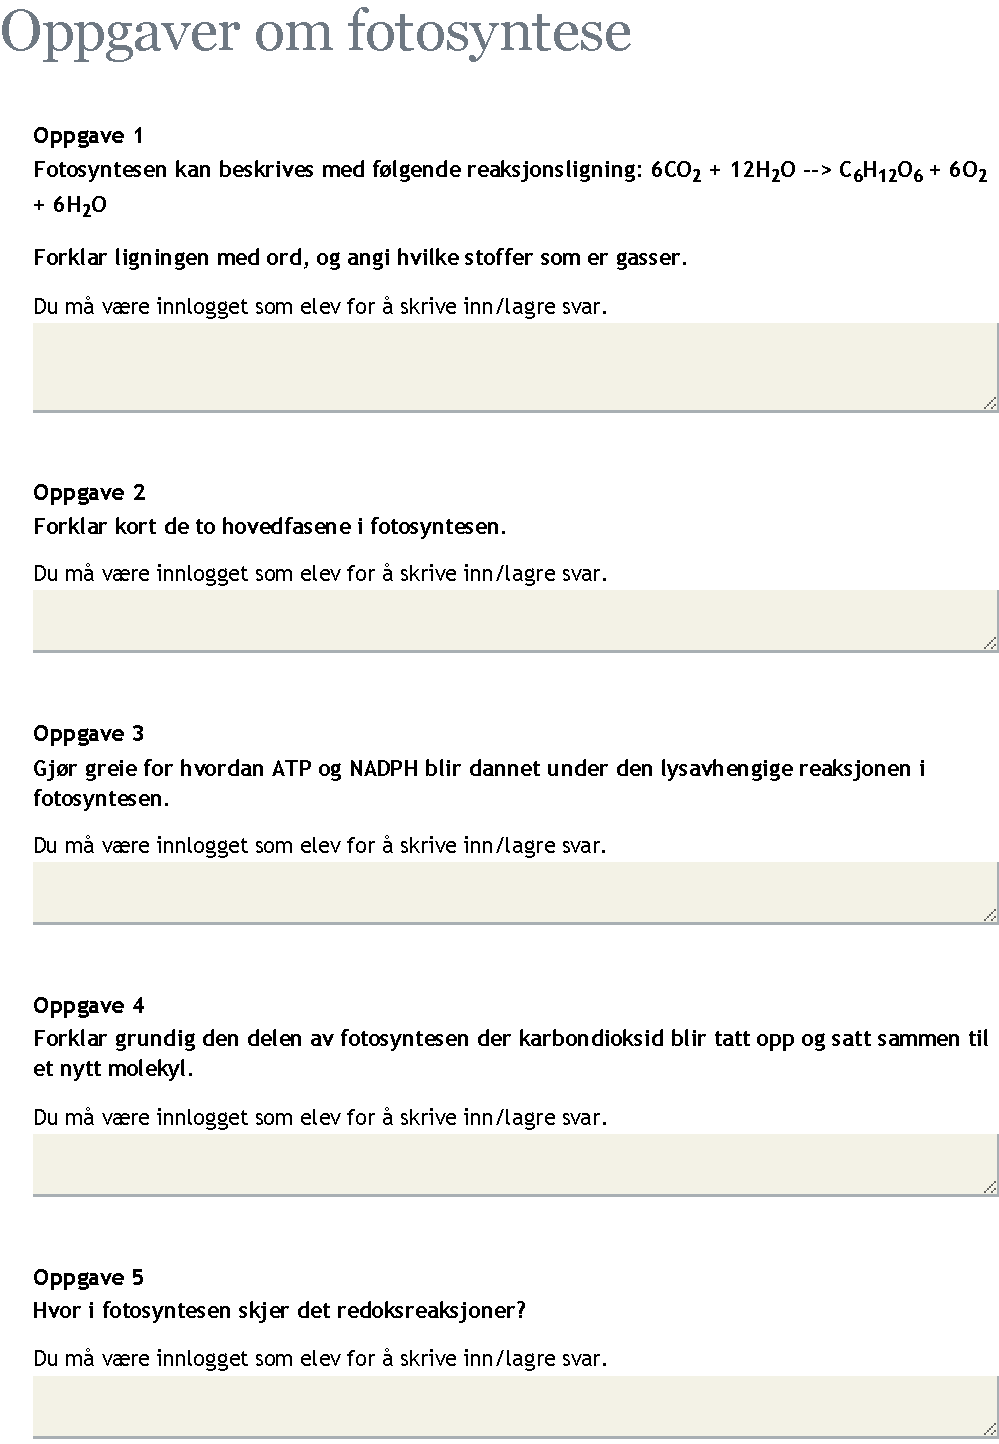
\includegraphics{img/theoretical/viten}} 
\fbox{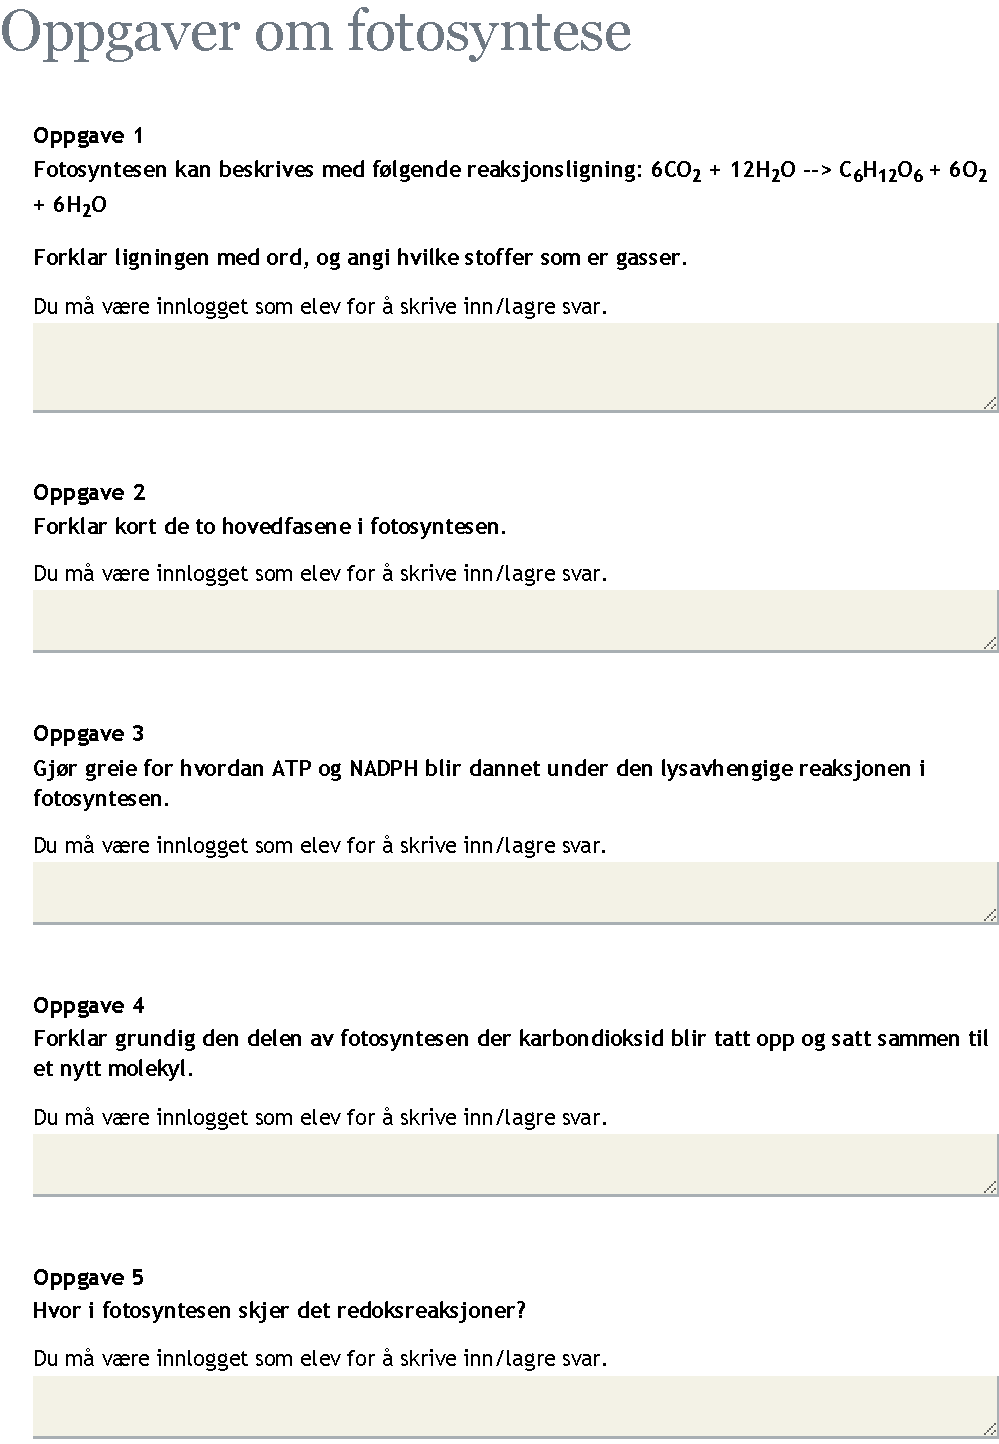
\includegraphics[width=1\textwidth]{img/theoretical/viten.pdf}}
\caption{Screenshot of viten.no showing student-role metaphor}
\label{fig:scrshotviten}
\end{figure}

Likewise \citet{jimenez2000doing} pose that "doing science" has an obstacle named "doing school". Where "doing science" refers to argumentation or dialog characterized by “construction, representation, evaluation of knowledge claims and investigative methods” \citep{jimenez2000doing}. While "doing school" refers to what actions and activities students and teachers do that instantiates rituals, routines and expectations in educational settings, e.g., review homework assignments, take lecture notes, take tests, complete lab activities etc. 

These school activities are often taken for granted by researchers, and serve as obstacles for "doing science", which tend to be a focus-area for researchers. Such research has contributed to the understanding of students' argumentation and knowledge claims, but as \citet*{furberg2008students} suggests; a more holistic view is needed to get a rich understanding of the complexity of students' meaning making. Meaning that both the dimension of "doing school" and the dimension of "doing science" needs to be taken into account. 

\subsection{Spontaneous and scientific concepts} \label{cha:spontaneous_scientific}
In the early stages of life, children learn for the most part by experience. Skills such as mastering the native language, walking, and running are learned through trial and error. This means that the knowledge of a concept is linked to the concrete experience where the concept was presented. A child who is presented with the concept of "brother" by a pointing gesture toward her brother, will at first only associate the word "brother" with that specific person. This is what \citeauthor{vygotsky2012thought} calls a \emph{spontaneous concept}.

An only child on the other hand, will be introduced to the concept of brother through other concepts. A parent can for instance say that "brothers are boys who have the same parents". The concept of brother will then be a general concept for the child, not linked to any concrete experiences, but to the concepts of "boys" and "parents". This is what \citeauthor{vygotsky2012thought} calls a \emph{scientificconcept}.

Spontaneous concepts are developed outside the conceptual framework and only linked to concrete experiences in the mind of the learner. If we presented the child having a brother with the abstract problem of a "brother's brother" \citep{vygotsky2012thought} he would become confused, as his only knowledge of the concept of brother is in situations with his own brother.

In contrast, scientific concepts are developed within a conceptual framework. They are immediately given a place within the system of concepts, i.e., explained by their relation to other concepts. As a result, the child is consciously aware and able to reflect on the concept \citep{van1998concept}. If we presented the only child with the abstract problem of a "brother's brother", he would most likely be able to solve it because of the concept's relation to other concepts in the mind of the child. 

Another example is how children develop a concept of time. In the early stages of life, a child may think that day and night is analogous to light and darkness. This is the spontaneous concept, which is saturated by experience. It is only later in life he learns the scientific concepts of the earth's rotation and its relation to the sun and the moon, which marks days and years. This information has not been appropriated by experience, as the child has not been to space and experienced it, the information is constructed using different signs linked together by the instructor. 

\begin{figure}
\centering
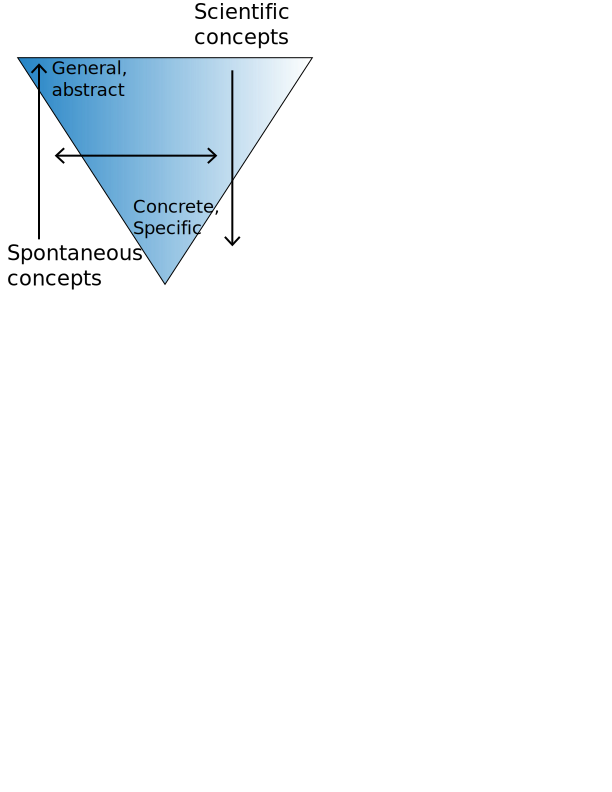
\includegraphics[width=0.6\textwidth]{img/theoretical/conceptpyramid.eps}
\caption{The concept pyramid}
\label{fig:conceptpyramid}
\end{figure}

The relationship between these two categories can be explained as an inverted pyramid. On the top we have the scientific concepts, which are general and abstract. And on the bottom we have the spontaneous concepts, which are specific and concrete. The concepts then move toward each other. The scientific concepts move downwards "toward greater concreteness" in a deductive manner, whereas the spontaneous concepts move "upward toward greater abstractness" \citep{vygotsky2012thought} in a inductive manner.

Even though the concepts move in opposite directions, there is a mutual dependency between them. In Vygotski{\u\i}'s terms: "In working its slow way upwards, an everyday concept clears a path for a scientific concept and its downward development". This means that "...the development of a spontaneous concept must have reached a certain level for the child to be able to absorb a related scientific concept" \citep[p. 194]{vygotsky2012thought}. It is therefore essential for the teacher to bring the spontaneous concepts up to a level that makes the scientific concept within reach for the student. By doing this, the student will have the experience, and the related concepts necessary for constructing knowledge of an abstract concept. 

This brings us to the zone of proximal development, as students who lack consciousness and control over the spontaneous concepts can "...find this control within the zone of proximal development" \citep[p. 194]{vygotsky2012thought}.

\subsection{Zone of proximal development}
Lev Vygotski{\u\i} was concerned with the relationship between learning and development, and argues that the theorists of his time such as Piaget, James and Koffka does not provide an adequate view of this. He finds that learning and development are interrelated, and that this relationship has some specific applications in school learning. \citep[p. 84]{vygotskiui1978mind} Thus, in order to describe these issues he introduces the concept zone of proximal development (ZPD), and defines it as follows:

\begin{quote}The distance between the actual developmental level as determined by independent problem solving and the level of potential development as determined through problem solving under adult guidance or in collaboration with more capable peers \citep[p. 86]{vygotskiui1978mind}.
\end{quote}

\begin{figure}
\centering
\includegraphics[width=0.7\textwidth]{img/theoretical/zpd.png}
\caption{The zone of proximal development \citep{wiki:zpd}}
\label{fig:zpd}
\end{figure}

The actual developmental level is in other words determined by looking at what a person can do alone. Vygotski{\u\i} found that this traditional way of determining a person's mental development does not hold in school learning, as it only describes what functions in a person that have already been matured. He therefore introduces a new developmental level, the potential development, which can describe the functions in a person that are in the process of maturation. The actual development is therefore the end product of developing, while the potential development is the state and process of developing. Teachers and instructors can then use the ZPD as a tool to delineate the immediate future of their students, i.e., their actual development of tomorrow.

Vygotski{\u\i} proposes further that ZPD is an essential feature of learning, which distinguishes learning from development, but at the same time provokes developmental processes that would not be possible without learning. In other words,

\begin{quote}It awakens a variety of internal developmental processes that are able to operate only when the child is interacting with people  in  his  environment  and  in  cooperation  with his peers \citep[p. 90]{vygotskiui1978mind}.
\end{quote}

By applying the ZPD to learning situations, the key takeaway is that the analysis alters the traditional view of knowledge or mastery, and shows that the constructed knowledge provides the basis for further development. A great example of this is the process of mastering native language, which initially is learned as a means of communication between the child and other people. The use of language first happens on a social level, in the interaction with people, and is later developed to internal speech and becomes a means to organize thought, i.e., an internal mental function. Vygotski{\u\i} calls this concept the \textit{duality of learning} \citep{vygotskiui1978mind}. 

Another classic example is that of a child trying to grasp a ball. At first the gesture means nothing to the child, but when the mother realizes that the gesture indicates something, the situation changes dramatically. When she gives him the ball, as a result of the hand gesture, the "...grasping movement changes to the act of pointing" \citep[p. 56]{vygotskiui1978mind}. This means that the operation that was initially an external activity is now "...reconstructed and begins to occur internally" \citep[p. 57]{vygotskiui1978mind}. Thus, \textit{externalization} precedes \textit{internalization}. 

With this in mind, a teacher can understand what developmental processes is maturing in their students, and from that give adapted challenges, show partial solutions and in general tailor what to say and teach next. From this perspective, development is lagging behind learning, and the challenge for the teacher becomes to teach ahead of development, but at the same time not too far ahead. This leads us to the concept of scaffolding, which can be argued to be a refinement of ZPD. 

\subsection{Scaffolding}
Vygotski{\u\i}'s zone of proximal development is the distance between what a person can do alone and what he can do with help from a more knowledgeable other (MKO). What types of help and how the MKO should provide it, has not been a focal point for Vygotski{\u\i}. Although \citeauthor*{wood1976role} does not reference to any Vygotski{\u\i}an literature, the term scaffolding introduced by them in 1976, bears resemblance to the very idea of ZPD. As they put it:

\begin{quote}Scaffolding consist essentially of the adult "controlling" those elements of the task that are initially beyond the learner’s capacity, thus permitting him to concentrate upon and complete only those elements that are within his range of competence \citep[p. 90]{wood1976role}.
\end{quote}

Thus, scaffolding can be applied by MKOs in order to keep the learning process within the learner’s ZPD. There is a is a nuanced balance for how much guiding is needed and a key point is that a person's ZPD is personal, thus a scaffold should be personally adjusted. An example can be if we were to teach two persons how to take a picture with a professional DSLR camera, one being an old woman (Mary) with little insight in technology, the other a young man (Ryan) who has grown up with technology. It is obvious that the two persons have different cultural backgrounds and taking a picture have different meanings to them, hence the tutoring of them need to be tailored differently. In the following section we will go through the six steps of scaffolding provided by \citet{wood1976role} using this example.

\begin{enumerate}
\item{} \emph{Recruitment} - We need to get the learners attention and interest in the task at hand. In our case this could be to show nice pictures of Mary's grandchildren to make her interested in taking nice pictures of them herself. For Ryan we could show the difference between pictures taken with an iPhone and a DSLR camera to make him understand the value of using a DSLR versus his iPhone.

\item{} \emph{Reduction in degrees of freedom} - The task must be narrowed down in order to provide a clear goal that can be reached. For Mary we can say that her task is to take a photo of her grandson playing in the garden with the use of auto-mode. And for Ryan, the task could be to take a landscape photo of his favorite view for his Facebook cover photo with the camera setting called A for aperture, which lets him control the depth of field - an important setting when photographing landscapes. 

\item{} \emph{Direction maintenance} - The learners must be kept on the path toward the goal, which implies a focus on motivation. Both to maintain progression and to keep a focus on the goal. From this point, scaffolding becomes an improvisation skill and it can be hard to plan ahead because of all the unforeseen things that can happen. Ryan can for example stop focusing on the landscape photo and instead take pictures of a car. While Mary starts looking at the pictures contained on the camera's memory stick. In this case one has to evaluate the goal versus the reduction in degrees of freedom. It might be that Ryan is more interested in taking pictures of cars, and since the main goal is to learn to take photos with a DSLR camera, an adjustment of the end product can be done. In Mary's case however, she might be easily distracted, and just needs someone to tell her to focus on taking pictures of her grandson. These are nuances that can be hard to spot, and requires a tutor with good improvisation skills.

\item{} \emph{Marking critical features} - Marking what the learner has done versus what is expected. This could be to show Mary that in her picture, she has left half her grandson's head out of the picture, and that she should try to capture a photo with the whole face visible. For Ryan it could be to point out that he has a very small depth of field in his photo, putting the trees in the foreground into focus, while leaving the mountains in the background blurred. Examples of correct solutions could be used to demonstrate the discrepancies between what the learner has produced and a correct solution.

\item{} \emph{Frustration control} - Balancing the dependency of the tutor and the independent problem solving. Both Mary and Ryan should be given some space to try taking photos, but we should at the same time be observant of when guiding or telling is needed. We could tell them to have the sun behind them to get the right light conditions, and hold the camera with two hands. The major risk here, is that the learner can become too dependent of the tutor, making it harder for the learner to achieve the goal, i.e., taking a picture alone at a later time.  

\item{}  \emph{Demonstration} - Showing a solution to the task, imitating the learner's earlier attempts and possibly correcting errors, with a hope that the learner will imitate back in a more correct manner. For Mary we could take a picture of her grandson, imitating her position, look for the sun, and then correct the position to get the sun behind us. Or for Ryan we could place the camera on a chair and use a timer to reduce movement of the camera, thereby allowing a slower shutter speed. This would allow a higher aperture, increasing the depth of field, giving focus to both the trees in the foreground and the mountains in the background. This might be supplemented by telling, to provide a context to the tutor's actions.
\end{enumerate}

As presented, some of these steps require planning while others require improvisation. Both the planning and improvisation turns out to be tailored to the specific situation at hand with all the complex contexts the learners bring with them to the situation. The steps can either be carried out manually by a tutor, or be mediated automatically by a computer-based system. \citet[p. 1]{fischer1991critics} presents one implementation of a computer-mediated scaffold where a critiquing system gives the user a "...reasoned opinion about a product or action generated by a human". Another example is from \citet{furberg2009socio} where prompts requiring user-input is used to promote student reflection. 

One important thing to note when reviewing the literature on scaffolding by \citet{wood1976role} and ZPD by \citet{vygotskiui1978mind} is that these studies are done on pre-school children. Critics may therefore argue that the concepts are not applicable to adult learning. Our stance is that when learning new concepts, both children and adults are alike. New and unknown concepts are new and unknown both for adults and children, and adults therefore become "as children" when introduced with new learning material. The concepts can therefore be used to analyze learning in all contexts where learning takes place. 

%Even though the six steps provided by \citet{wood1976role} can be considered as a framework for scaffolding, it is still quite complex and demands careful consideration by the teacher or the designers of the computer based scaffold.  

\section{Multiple external representations}
Multiple external representations (MER) are often used for conveying information. Textbooks and manuals contain images and illustrations, maps show different information in different ways, and whiteboards are used in addition to speech. With digital technology the possibilities of MER are expanded to include dynamic linking between the representations, and the representations can show dynamic information that is not available in the real world, e.g., visualizing the flow of oxygen. 

In an effort to identify the features of MER, \citet{ainsworth1999functions} has developed a classification framework. She suggests that MER can serve primarily three different purposes in learning situations:
\begin{enumerate}
\item{} \emph{Complementary roles} - Different representations can focus on different aspects of the phenomenon under study, or they can contain different information of the same phenomenon. E.g., a topographic map in addition to a road map. 
\item{} \emph{Constrain interpretation} - One representation can be used to constrain the interpretation of the other. E.g., the text “the fork lies next to the spoon”. It is impossible to tell which side the fork is on, but by presenting an illustration of the example, the representation will constrain the interpretation of the text. 
\item{} \emph{Construct deeper understanding} - MER can be used to "...promote abstraction, to encourage generalization and to teach the relation between representations" \citep[p. 141]{ainsworth1999functions}. 
\end{enumerate}

The three different roles presented above are also the benefits of using MER. Complementary roles can support students to make up for insufficient knowledge of one representation by using another, constrain interpretation can “support the learners’ reasoning about the less familiar representation” \citet{ainsworth1999functions}, and finally the learners can gain deeper understanding of the domain by translating between representations \citep{van2006supporting}. 

On the other hand, when learners are faced with MER they must also undertake additional tasks as to understand the phenomenon or domain in question. This may lead to a heavy cognitive load, which "...may leave less resources for actual learning" \citetext{\citealp{sweller1988cognitive,sweller1989cognitive}, referenced in \citealp{van2006supporting}, p. 200}. A key issue is then to reduce the cost for learners associated with MER, while keeping the benefits. 

\section{Inquiry learning}
According to \citet{prince2006inductive} science has traditionally been taught in a \textit{deductive} manner. In the same way as Sherlock Holmes collects piece by piece to form a theory, the students collect pieces of models and illustrations to grasp a scientific concept. Little attention is paid to why the students should learn the material, apart from having to perform on tests.

On the other hand we have the \textit{inductive} ways of teaching and learning. Instead of beginning with the theory, the students are presented with some sort of task, which becomes the motivation to learn the tools required to solve the task. Examples of this can be to make a battery in a science class, or finding out why potato-chips bags seem more inflated on the top of a mountain than by the sea.

Inquiry learning involves giving the students "...questions to be answered, problems to be solved, or a set of observations to be explained" \citep[p. 127]{prince2006inductive}, or in other words: giving the students incentives to ask for information. There are several other inductive learning methods, such as problem-based learning, discovery learning and project-based learning, which all can be explained with the same statements as inquiry learning. Inquiry learning can therefore be seen as an umbrella term for inductive learning methods. \citep{prince2006inductive}

\citeauthor*{staver1987analysis} \citetext{\citeyear{staver1987analysis}, referenced in \citealp{prince2006inductive}} differentiates between \emph{structured inquiry} (e.g., tutorials), \emph{guided inquiry} and \emph{open inquiry}. Depending on the student's developmental level, different framings of the inquiry process are needed. To scaffold the inquiry learning process is not an easy task. In a review article, \citet{de1998scientific} identifies four problems that learners may encounter when engaging with inquiry learning: \textit{hypothesis generation}, \textit{design of experiments}, \textit{interpretation of data}, and \textit{regulation of discovery learning}. They continue to argue for the need of supporting students during the process of scientific inquiry, providing scaffolds for each of these problems. The challenge then becomes to "...guide students to the "right" path, but at the
same time letting them discover and make the discovery their own" \citep[p. 247]{kluge2010simulation}. In other words the students need to be steered toward the interesting discoveries, but at the same time have the freedom to explore and not be commanded in any way.

\subsection{Misconceptions}
Misconceptions appear in most educational contexts. According to \citet[p. 437]{gomez2008elementary} students have "...qualitative differences in his or her understanding of science that is often inconsistent with what the teacher intended through his or her instruction". These are often deeply rooted, and remain intact even after instruction. This becomes especially relevant when dealing with inductive learning methods, as the students are given more freedom to explore their own ideas, and thus more freedom to pursue tracks that may lead to different conclusions than the ones intended by the instructor.

The term itself has been given many labels in research literature, depending on the focus: "alternative frameworks", "preconceptions", and "student ideas" are just some of them. An important factor here is how misconceptions are perceived. Are they resources for learning, or obstacles that the learner has to overcome? If we look at meaning making from a constructivist point of view, advanced knowledge is built upon prior understanding. Misconceptions then become "...faulty extensions of productive prior knowledge" \citep[p. 152]{smith1994misconceptions}.

To simply write misconceptions off as mistakes is, according to \citet{smith1994misconceptions}, a too narrow view in their role in learning. If we take the example of stating that "multiplication makes numbers larger", it is indeed an accurate explanation of most multiplication pieces. The problem arises in the few cases where we multiply by non-natural numbers. The conception that leads to erroneous conclusions in some contexts can be quite useful in others \citep{smith1994misconceptions}. The misconceptions are therefore for the students "...conceptions in their own right with plausibility and at explanatory power" \citetext{\citealp{smith1994misconceptions}, referenced in \citealp{larkin2012misconceptions}, p. 928}. 

%As stated before, the goal then becomes to scaffold the students in such a way that the interesting discoveries are made, and the misconceptions discussed. 

\section{Outline of concepts for analysis}
We have now introduced the sociocultural perspective and several important concepts within and besides its frames. Further we will use this perspective and the following concepts to guide our research design and discuss our findings: \emph{zone of proximal development}, \emph{scaffolding}, \emph{spontaneous and scientific concepts}, \emph{multiple external representations}, \emph{institutional practices}, \emph{inquiry learning}, and \emph{misconceptions}.

 %!TEX root = ../document.tex
\chapter{Empirical settings and methods}
In this chapter...

\section{Empirical setting}
The collection of data material used in this thesis took part in the late autumn, 2013, at a high school located in the centre of Oslo. The school is in the upper third on the grade scale, with a limit of 43.5 points for admission in 2010/2011 \citep{utdanningsetaten}. Therefore the students at this school are mostly high achievers. 

Contact with the school was first initiated through Intermedia, and a presentational flyer was sent as an explanation of the project (_____appendix_____). Luckily our request coincided perfectly with a 2 week time frame for reviewing photosynthesis in one of the teacher's classes, and he was therefore quite eager to use our application in class. 

The class selected for the experiment was a biology class at the highest level offered at the school, biologi 2, which has an extensive curriculum covering e.g photosynthesis, enzymes and energy transmitters. The students were between 17 and 18 years of age, and for the main part most of the 20 students taking the class were present. All the students aggred to participate in the study, but due to technical limitations, data collection was only done with a small sample of the group. 


\def\arraystretch{1.8}
\begin{table}
    \begin{tabular}{@{}lp{250pt}@{}}\toprule
    Sensor               & Description \\ \midrule                                                                                                  
    TSL2561              & Digital luminosity sensor. Measures light in lux from 300-1100nm.                                            \\ 
    RHT03                & Digital humidity and temperature sensor. Measures relative humidity and temperature in celsius.              \\ 
    DS18B20              & Digital waterproof temperature sensor. Measures temperature in celsius                                       \\ 
    DFRobot sku:sen0114  & Analog soil moisture sensor. Returns values between 0 and 900 depending on electrical conductivity of soil.  \\ \bottomrule
    \end{tabular}
    \caption{Sensors used in the application}
\end{table}


With the advent of the \emph{“internet of things”}, sensors are becoming available in many different forms and packages. Just as LEGO-pieces they can be used in a wide range of applications. From automating tasks such as keeping a steady indoor-temperature, to measuring variables which we as humans cannot see. 

For this application we did a short review of the available off-the-shelf packages available on the market. 

The sensors are able to capture information about the environment and transform it to data variables which we can store and categorize. In total there are five different sensors connected to the plant, or in the plant’s vicinity: soil moisture, soil temperature, air temperature, humidity, and light. 


(write something about the sensortag)

Simplified we can say that the sensors function in the same way as a volume controller on an amplifier. On an amplifier one can adjust the volume by varying the resistance in the signal going to the speakers. If we turn the volume up, the resistance goes down, which lets more power through to the speakers. And if we turn the volume down, the resistance goes up which lets less power flow to the speakers. The concept with sensors is the same, only that instead controlling resistance with a volume knob, it is controlled by light, moisture or other environmental variables. 

For a good example, lets look at how the temperature sensors work. The resistors used in the temperature sensors are called “thermistors”, and the way they operate is by varying the resistance according to the temperature. Since we already know how many volts we are sending to the thermistor on the one end, we can use the amount of volts we get back to calculate the resistance. In our application this is done by a voltage divider which uses a formula as follows: 

\begin{equation}
U_{out}=\frac{R_{2}}{R_{1}+R_{2}}\cdot U_{in} 
\label{eq:vdiv1}
\end{equation}
Where $V_{out}$ is voltage out, $U_{in}$ is voltage in, $R_{1}$ is a given resistance, and $R_{2}$ is the resistance we want to calculate. For this example let's assume that $U_{in} = 5_{v}$, $U_{out} = 2_{v}$, and $R_{1} = 1K\Omega$. We solve this equation with regard to $R_{2}$
\begin{equation}
R_{2} = \frac{U_{out} \cdot R_{1}}{U_{in}-U_{out}}
\end{equation} 

\begin{equation}
R_{2} = \frac{2V \cdot 1000\Omega}{5V-2V}
\end{equation} 

\begin{equation}
R_{2} = \frac{2000\Omega}{3}
\end{equation} 

\begin{equation}
R_{2} = 667\Omega
\end{equation} 

Then we can see that the calculated resistance is 667$\Omega$. This value can then be mapped to the correct unit of measure, in this case Celsius or Fahrenheit. 

As we are using digital sensors, all of these calculations are done internally in the sensors, and coded into a digital signal. This signal, consisting of 1s and 0s, is then passed onto the next unit in our system, the Arduino.  

\subsection{Arduino}
(Write about embedded systems. What other alternatives are there to the Arduino? )

Arduino is an open-source prototyping platform which makes it easy to interface low-level electronics (e.g sensors) with higher-level electronics (e.g computers). The core part of the Arduino is an Atmel\texttrademark Atmega microcontroller which can be programmed by a computer over usb, using the Arduino programming language and the Arduino development environment \citep{arduino}.

We have used an Arduino Uno which has 13 digital input output pins (GPIO), five analog inputs, i2c inputs, and USB for serial communication. The DSB18B20 soil temperature sensor and RHT03 temperature and humidity sensor are connected to the digital inputs through a 1K(ohm) pullup resistor. The pullup resistors are used to keep the voltage sent to the arduino from fluctuating when the sensor is not sending any data. The TSL2561 luminosity sensor is connected to the A4/SDA and A5/SDL ports of the Arduino as it communicates over the i2c protocol. And the DFRobot soil moisture sensor is connected to A3 (Analog input 3) as it outputs analog voltage.  

\begin{figure}
\centering
\includegraphics[width=1\textwidth]{img/hardware/Arduino_and_sensors_schem.png}
\caption{Schema diagram of Arduino sensor wiring}
\label{fig:arduino}
\end{figure}

The community surrounding Arduino is quite large, and therefore we were able to find pre-written libraries for communicating with the different sensors. This has made the task of converting the digital signal to the correct units (celsius, relative humidity, lux) and levels a breeze. 

In the case of the soil moisture sensor, it does not output soil moisture in any kind of universal unit. Therefore we measured the resistance in air (high resistance), and in water (low resistance), and let these be the high and low points of a new unit called arbitrary moisture units (AMU).

The code residing in the arduino runs a simple loop where it waits for a special character sent over serial communication through USB. If it receives this character it reads all the sensor values, and sends them back to the next logical unit: the Raspberry Pi

\subsection{Raspberry Pi}
(Why raspberry? Beagleboard?)
The Raspberry Pi is a “cheap, accessible, programmable computer” \citep{raspberrypi} which is roughly the size of a credit card. Our model was released early 2012, and contains two usb ports, audio, sd-card slot, and several GPIO-pins. The devices connected to it are: wireless network adapter, high-definition webcamera, and the Arduino. The operating system running on it is a port of Debian Linux optimized for the Raspberry, called Raspbian. 

(illustration of raspberry)

The GPIO-pins on the raspberry works almost in the same fashion as the Arduino’s digital input output pins. Thus we could in theory simplified the hardware by omitting the Arduino. The main reason for not doing this is that the Raspberry does not have an analog to digital converter (ADC). Therefore we would have to make a complex circuit involving an ADC to interface the Raspberry with the soil moisture sensor. In addition, we would most likely face timing issues. When we ask the digital sensors for data, they send the response immediately. If the unit receiving is not available to read the data, it gets lost. This can be a problem when using a high-level computer, as it performs multiple other tasks in addition to reading sensordata. 

\subsubsection{Operation}
After booting up an endless loop bash-script is called. The script snaps a photo of the plant using the webcam, and then runs a python-script responsible for collecting sensordata. Since we sometimes can get erroneous values from the sensors, we read 15 values and upload the median value.

%http://en.wikibooks.org/wiki/LaTeX/Packages/Listings
\lstset{language=Python} 
\begin{figure}
\begin{lstlisting}
//instantiate lists
airtemp = []
humidity = []
light = []
soiltemp = [] 

for x in xrange(1,15): 
	ser.write("r") //Ask Arduino for data
	variables = ser.readline() //Read the data
	sensorReadings = variables.split('|') //Split string on |

	airtemp.append(float(sensorReadings[0]))
	humidity.append(float(sensorReadings[1]))
	light.append(float(sensorReadings[2]))
	soiltemp.append(float((sensorReadings[3])[:-2])) 

//calculate and post the median using numpy
postData(np.median(airtemp),np.median(humidity),np.median(light),np.median(soiltemp)) 
\end{lstlisting}
\caption{Reading sensor values from Arduino on Raspberry PI}
\label{fig:raspberrycode}
\end{figure}

These values, along with the photo of the plant, are then passed on to the next instance, the API, using pythons HTTP-library urllib2. 

\section{Data processing and database}
When the data has been gathered at the low level hierarchy, it is stored in the cloud. This is done by posting the data to an API on our web server. The main function of an API is to be a mean of communication between software, in our case the data collector and the user interface. After some research on web-API design, we decided that a REST architectual style was the way to go. 

\subsection{Representational State Transfer (REST)}
REST is an architectual style for distributed hypermedia systems \citep{fielding2000architectural}. In Fielding's dissertation, he writes about the interaction constraints of REST that is introduced in order to limit how a distributed system can be constructed. 
=======
\subsection{Planning}
The planning of the project was done by us in conjuction with the teacher responsible for the for the biology class. An initial plannign meeting was held at the school around one week before the experiments started. There we gave the teacher a thorough introduction of the system, and presented some ideas for expirements the students could perform using our system as platform. This involved:
>>>>>>> 4056fd08d59c7d41cdee9e1f90c94e5ae23dbd4d

\begin{enumerate}
\item{Present the application in class}
\item{Initiate an experiment using the application. Related to e.g soil moisture, light intensity, light quality, or temperature}
\item{Have a one hour session where the students work with text tasks realted to the experiment}
\end{enumerate}

The teacher then suggested that we could conduct two experiments, so the students could work on the relations between the different external factors effect on photosynthesis. As the system records a range of different variables, it would be possible to keep the environment relatively controlled, or at least point to factors which could be sources of error in the experiment. 

We agreed that the factor where we could get the most interesting result was to vary the light intesity and the light quality (wavelength). The first experiment would then involve keeping the plant located in a window facing west, receiving sunlight and light from the fluorescent indoor-lighting. In the second experiment we would plant new seeds, and relocate the plant to a (presumably) light proof cupboard. The plant would then only be given green light, with a known wavelength. Each of the experiments would have a duration of approximately one week. 

\subsection{Execution pow pow ?}
The project was presented and the first experiment initiated by one of the students on friday 25th of october. This went on until friday 1st of november when the second experiment was initiated. The second experiment went on until wednesday 13th of november when the primary data collection session started. During the experiments we were present at four separate occations, observing what the teacher was focusing on, and what kind of questions/which part of the photosynthesis the students found most difficult. In addition to answering questions about the system, and if/how the system was used in the education. 

\subsection{Data collection}


Our main data material consists of x hours of video from the session... blabla

\section{Analytical Procedures}

\subsection{Ethics}




 %!TEX root = ../document.tex
\chapter{Data \& Analysis}
In this chapter we will present the findings from our case study ...

\section{Hypothesis generation}

\subsection{Context}
In table~\ref{excerpt:expectations1} the students are discussing assignment 1a, and are talking about what they thought would happen to the plant which only got green light. While discussing they are also describing the what the conditions for the plant was. The plant from the closet is in front of them on the table, but they do not know which plant it is. 
\subsection{Raw data}


\def\arraystretch{1.5}
\begin{table}
\begin{adjustwidth}{-4em}{-4em}
\begin{center}
\begin{tabular}{r l p{9cm} p{4cm} } \toprule
	Time &  Who &  Speech  & Action\\ \midrule  

	2:16 %time
	&Siri %name
	&\parbox[t]{9cm}{\raggedright .. det var det planten stod i skapet også skulle det være bare grønt lys på den ... men det kan jo hende for eksempel at det kom litt annet lys inn i skapet også .. så da er det ikke sikkert at det bare bar grønt lys ..  %speech 
	}&\parbox[t]{4cm}{\raggedright peker på skapet %action 
	}\\

	2:31 %time
	&Nora %name
	&\parbox[t]{9cm}{\raggedright  %speech 
	}&\parbox[t]{4cm}{\raggedright nikker %action 
	}\\

	2:31 %time
	&Siri %name
	&\parbox[t]{9cm}{\raggedright og planten tar jo opp littegrann grønt lys også, men ikke så mye .. så derfor kunne det hende atte den ikke vokste like my.. eller jeg trodde at den ikke ville vokse like mye i skapet .. siden da fikk den bare grønt lys ...  %speech 
	}&\parbox[t]{4cm}{\raggedright  %action 
	}\\

	2:46 %time
	&Nora %name
	&\parbox[t]{9cm}{\raggedright ... mmm ... %speech 
	}&\parbox[t]{4cm}{\raggedright  %action 
	}\\

	2:47 %time
	&Siri %name
	&\parbox[t]{9cm}{\raggedright eller neste bare grønt lys ihvertfall ... men hvor mye vokste den egentlig? er det den ((refererer til planten på bordet)) som stod i skapet? %speech 
	}&\parbox[t]{4cm}{\raggedright peker på planten som står på pulten %action 
	}\\

	2:52 %time
	&Sjur %name
	&\parbox[t]{9cm}{\raggedright ja %speech 
	}&\parbox[t]{4cm}{\raggedright  %action 
	}\\

	2:53 %time
	&Nora %name
	&\parbox[t]{9cm}{\raggedright OJ(!) %speech 
	}&\parbox[t]{4cm}{\raggedright  %action 
	}\\

	2:53 %time
	&Siri %name
	&\parbox[t]{9cm}{\raggedright Den har jo vokst ganske mye %speech 
	}&\parbox[t]{4cm}{\raggedright smiler %action 
	}\\
	
	\bottomrule
\end{tabular}
\end{center}
\end{adjustwidth}
\caption{Excerpt from exercise 1}
\label{excerpt:expectations1}
\end{table}

\subsection{Explanation}
Siri had an expectation that the plant from the closet would not grow as much as the plant from the window, and she is explaining why she thinks that. At the same time, she knows from looking at the system earlier, that the plant have grown, so she tries to explain why it has grown at all. 


\section{Hypothesis generation}

\subsection{Context}
After looking at the plant on the table the student wanted to know if the stems on the plants in the window where white as the stems in the closet. They opened monoplant and navigated to the videolist, where they got an overview over the looks of the two different plants. They checked the color of the stems, and opened a video from 31th of October, then pressing play. This is when Fredrik starts to talk in table~\ref{excerpt:hypothesis1}.



\subsection{Raw data}


\def\arraystretch{1.5}
\begin{table}
\begin{adjustwidth}{-4em}{-4em}
\begin{center}
\begin{tabular}{r l p{9cm} p{4cm} } \toprule
	Time &  Who &  Speech  & Action\\ \midrule  

	3:24 %time
	&Fredrik %name
	&\parbox[t]{9cm}{\raggedright mhm ... mmja så da er det jo egentlig ganske ... ja ikke så stor forskjell da på de som stod ...  i skapet ((peker på planten på border)) og de som stod i vinduskarmen hvis man bare ser på ...  utseende %speech 
	}&\parbox[t]{4cm}{\raggedright Dette sies mens Siri starter videoen, hun stopper også videoen før de har sett den halvferdig. %action 
	}\\

	3:37 %time
	&Siri %name
	&\parbox[t]{9cm}{\raggedright ja .. men da ville jeg kanskje tenke at det kan hende at det kom inn annet lys enn det grønne lyset også. siden de har vokst så bra, og at de vokser bedre hvis de får flere.. lys i flere bølgelengder enn bare grønt lys %speech 
	}&\parbox[t]{4cm}{\raggedright Stemmeleiet går opp mot slutten av setningen, og løfter blikket fra arket for å få bekreftelse %action 
	}\\

	... %time
	&... %name
	&\parbox[t]{9cm}{\raggedright \emph{Intervensjon hvor Sjur introduserer og forklarer bildet av lysspekteret på oppgavearket.} %speech 
	}&\parbox[t]{4cm}{\raggedright  %action 
	}\\

	4:14 %time
	&Siri %name
	&\parbox[t]{9cm}{\raggedright mhm ... der er det jo litt blått lys og sånt også. %speech 
	}&\parbox[t]{4cm}{\raggedright Peker på det blå lyset i illustrasjonen øverst på oppgavearket %action 
	}\\

	4:18 %time
	&Nora %name
	&\parbox[t]{9cm}{\raggedright ja så det er ikke bare rent grønt … %speech 
	}&\parbox[t]{4cm}{\raggedright  %action 
	}\\

	4:20 %time
	&Fredrik %name
	&\parbox[t]{9cm}{\raggedright ... ja det er jo ikke bare på 500 circa ((referer til bølgelengde)), det er jo et stort område %speech 
	}&\parbox[t]{4cm}{\raggedright Holder hendene fra hverandre som om han signaliserer hvor langt noe er. %action 
	}\\

	4:26 %time
	&Siri %name
	&\parbox[t]{9cm}{\raggedright mhm, og planten tar jo ihvertfall opp veldig mye blå .. blårlilla lys ... %speech 
	}&\parbox[t]{4cm}{\raggedright  %action 
	}\\

	4:31 %time
	&Fredrik %name
	&\parbox[t]{9cm}{\raggedright ... mhm ... %speech 
	}&\parbox[t]{4cm}{\raggedright  %action 
	}\\

	4:32 %time
	&Siri %name
	&\parbox[t]{9cm}{\raggedright så da har den sikkert kunnet utnytte mye av dette her. %speech 
	}&\parbox[t]{4cm}{\raggedright peker på det blå spekteret i illustrasjonen øverst på oppgavearket %action 
	}\\


	\bottomrule
\end{tabular}
\end{center}
\end{adjustwidth}
\caption{Excerpt from hypothesis generation 1}
\label{excerpt:hypothesis1}
\end{table}

\subsection{Explanation}
Fredriks observation on the appearance of the plants breaks Siris expectation that the plant in the closet would not grow as much as the on in the window. Siri starts to explain why this could have happened by talking about light in different wavelengths, but without explaining why this has any effect on growth, only stating that it has an effect.
Sjur drops in and introduces the illustration of the green light on the paper as it appears as if they have not seen this yet. This gives the students more hold in Siris explanation that it might not only be green light in the closet, as the green lamp produces some light in the blue specter. So they now have two possible explanations to why the plants have grown (in their eyes) the same amount. Firstly, there might have been some light pollution coming into the closet, and secondly the green light is not purely green.

\section{Hypothesis generation}

\subsection{Context}
In table~\ref{excerpt:disconfirmation1} the students have been looking at the movements of the two plants, and have observed that the plant in the window are moving towards the sun, a so called heliotropism. They are now observing that the plant in the closet is just growing straight up without any large movement like the other plant. Suddenly Nora observes that the plant is growing a lot more than the window plant.
\subsection{Raw data}


\def\arraystretch{1.5}
\begin{table}
\begin{adjustwidth}{-4em}{-4em}
\begin{center}
\begin{tabular}{r l p{9cm} p{4cm} } \toprule
	Time &  Who &  Speech  & Action\\ \midrule  

	7:46 %time
	&Nora %name
	&\parbox[t]{9cm}{\raggedright Jeg føler at de vokser veldig mye inni ... skapet eller er det? ... %speech 
	}&\parbox[t]{4cm}{\raggedright  %action 
	}\\

	7:51 %time
	&Siri %name
	&\parbox[t]{9cm}{\raggedright Ja det virka som om de vokste ... %speech 
	}&\parbox[t]{4cm}{\raggedright  %action 
	}\\

	7:53 %time
	&Nora %name
	&\parbox[t]{9cm}{\raggedright ... ser ut som de ble lenger lissom ... %speech 
	}&\parbox[t]{4cm}{\raggedright  %action 
	}\\

	7:53 %time
	&Siri %name
	&\parbox[t]{9cm}{\raggedright ... enda mer der. %speech 
	}&\parbox[t]{4cm}{\raggedright  %action 
	}\\

	7:54 %time
	&Fredrik %name
	&\parbox[t]{9cm}{\raggedright ja %speech 
	}&\parbox[t]{4cm}{\raggedright  %action 
	}\\

	7:56 %time
	&Siri %name
	&\parbox[t]{9cm}{\raggedright ... enn ute, at de ble mye lengre. %speech 
	}&\parbox[t]{4cm}{\raggedright  %action 
	}\\

	7:59 %time
	&Fredrik %name
	&\parbox[t]{9cm}{\raggedright mhm. %speech 
	}&\parbox[t]{4cm}{\raggedright  %action 
	}\\

	8:01 %time
	&Siri %name
	&\parbox[t]{9cm}{\raggedright Kanskje de fokuserer veldig på å vokse oppover når lyset er rett over dem.. at de vokser rett oppover ((fører hånden oppover)) i stedet for å følge lyset og gå lissom sånn sakte oppover ((snurrer hånden sakte oppover)) %speech 
	}&\parbox[t]{4cm}{\raggedright  %action 
	}\\
	
	
	\bottomrule
\end{tabular}
\end{center}
\end{adjustwidth}
\caption{Excerpt from disconfirmation of growth}
\label{excerpt:disconfirmation1}
\end{table}

\subsection{Explanation}
Siri starts at once to generate a hypothesis for why the plant in the closet are growing more than the one in the window. \sout{It might be because it is hard for her to realize that her expectations where wrong and she is trying to cope with her misconception of plants growing in green light.} Basically what she is saying is that heliotropism makes the plant in the window grow slower because it has to move after the sun, and since the plant in the closet can grow straight up, it can grow faster. 

\section{Hypothesis generation}

\subsection{Context}
Morten has asked if the students has looked at the graphs below the video, and the students have in response looked into the graphs and observed that the light graph is really different in the two enviroments. In  table~\ref{excerpt:hypothesis2} Sjur then asks the question they wondered about earlier again to see if the graphs can help them test their hypothesis. 

\subsection{Raw data}

\def\arraystretch{1.5}
\begin{table}
\begin{adjustwidth}{-4em}{-4em}
\begin{center}
\begin{tabular}{r l p{9cm} p{4cm} } \toprule
	Time &  Who &  Speech  & Action\\ \midrule  

	9:21 %time
	&Sjur %name
	&\parbox[t]{9cm}{\raggedright Men hvorfor tror dere den i skapet strekker seg så mye, den som fikk grønt lys ... %speech 
	}&\parbox[t]{4cm}{\raggedright Nora snur seg mot Sjur som står bak gruppen %action 
	}\\

	9:26 %time
	&Nora %name
	&\parbox[t]{9cm}{\raggedright De skal jo bare vokse oppover da, eller den vokser bare oppover så.. %speech 
	}&\parbox[t]{4cm}{\raggedright Siri snur seg også %action 
	}\\

	9:30 %time
	&Sjur %name
	&\parbox[t]{9cm}{\raggedright ja? %speech 
	}&\parbox[t]{4cm}{\raggedright  %action 
	}\\

	9:31 %time
	&Nora %name
	&\parbox[t]{9cm}{\raggedright Da.. har den mye energi til det? %speech 
	}&\parbox[t]{4cm}{\raggedright  %action 
	}\\

	9:33 %time
	&Siri %name
	&\parbox[t]{9cm}{\raggedright Ja kanskje den fokuserer på å vokse rett oppover ((tar hånden oppover)) når lyset står der hele tiden.. åja! også om natta så er det jo ikke sol, så da … %speech 
	}&\parbox[t]{4cm}{\raggedright  %action 
	}\\

	9:43 %time
	&Nora %name
	&\parbox[t]{9cm}{\raggedright Da vokser den jo ikke opp... %speech 
	}&\parbox[t]{4cm}{\raggedright ser usikkert mot sjur etterhvert %action 
	}\\

	9:44 %time
	&Fredrik %name
	&\parbox[t]{9cm}{\raggedright mhm %speech 
	}&\parbox[t]{4cm}{\raggedright  %action 
	}\\

	9:45 %time
	&Siri %name
	&\parbox[t]{9cm}{\raggedright da vokser den ikke etter lyset på en måte %speech 
	}&\parbox[t]{4cm}{\raggedright litt usikker i stemmen %action 
	}\\

	9:47 %time
	&Nora %name
	&\parbox[t]{9cm}{\raggedright Ja altså den vokste jo dag og natt .. i .. skapet %speech 
	}&\parbox[t]{4cm}{\raggedright  %action 
	}\\

	9:50 %time
	&Siri %name
	&\parbox[t]{9cm}{\raggedright mhm, for det var lys der hele tiden ... så den strakk seg hele tiden etter lyset %speech 
	}&\parbox[t]{4cm}{\raggedright  %action 
	}\\

	\bottomrule
\end{tabular}
\end{center}
\end{adjustwidth}
\caption{Excerpt from hypothesis 2}
\label{excerpt:hypothesis2}
\end{table}

\subsection{Explanation}
Here they found that since the plant in the closet got light all night and all day, it got more light than the plant in the window which got light only during the day.

\section{Hypothesis generation}

\subsection{Context}
Earlier Morten explicitly told the group to look at the light graphs again, however, the group only stated the fact that the window plant got a lot of light during the day, but nothing at night, where as the plant in the closet got a constant amount of light.
table~\ref{excerpt:hypothesis2} 

\subsection{Raw data}

\def\arraystretch{1.5}
\begin{table}
\begin{adjustwidth}{-4em}{-4em}
\begin{center}
\begin{tabular}{r l p{9cm} p{4cm} } \toprule
	Time &  Who &  Speech  & Action\\ \midrule  

	10:49 %time
	&Sjur %name
	&\parbox[t]{9cm}{\raggedright mens den andre gjerne .. nesten ligge på null heile veien da .. (?) %speech 
	}&\parbox[t]{4cm}{\raggedright Fredrik og Nora snur seg. Nora nikker %action 
	}\\

	10:53 %time
	&Siri %name
	&\parbox[t]{9cm}{\raggedright Å ja! det var jo lavere lys der, men så blir det veldig mye lys her når det først er lys. %speech 
	}&\parbox[t]{4cm}{\raggedright har et ganske bekymret ansiktsuttryk mens hun prøver å forstå hva hun sier. %action 
	}\\

	11:11 %time
	&Sjur %name
	&\parbox[t]{9cm}{\raggedright Men hvis dere ser på baksiden av det oppgavearket %speech 
	}&\parbox[t]{4cm}{\raggedright Peker mot arket. Nora snur arket %action 
	}\\

	 %time
	& %name
	&\parbox[t]{9cm}{\raggedright  %speech 
	}&\parbox[t]{4cm}{\raggedright  %action 
	}\\

	 %time
	& %name
	&\parbox[t]{9cm}{\raggedright  %speech 
	}&\parbox[t]{4cm}{\raggedright Lærer kommer bort %action 
	}\\

	11:20 %time
	&Lærer %name
	&\parbox[t]{9cm}{\raggedright Går det bra eller %speech 
	}&\parbox[t]{4cm}{\raggedright kommer bort til bordet og lener seg på det. %action 
	}\\

	11:23 %time
	&Siri %name
	&\parbox[t]{9cm}{\raggedright mmm, ja %speech 
	}&\parbox[t]{4cm}{\raggedright  %action 
	}\\

	11:24 %time
	&Lærer %name
	&\parbox[t]{9cm}{\raggedright skjønner dere ... har dere funnet forklaring på alle spørsmålene? %speech 
	}&\parbox[t]{4cm}{\raggedright  %action 
	}\\

	11:26 %time
	&Alle jentene %name
	&\parbox[t]{9cm}{\raggedright *** vi prøver ... %speech 
	}&\parbox[t]{4cm}{\raggedright snakker i munnen på hverandre %action 
	}\\

	11:27 %time
	&Siri %name
	&\parbox[t]{9cm}{\raggedright Jeg tror kanskje jeg har en ide om det med at den her ute ((peker mot vinduet, refererer til planten i vinduet)) ikke vokser like høyt, eller så fort ihvertfall.. fordi atte når det kommer veldig mye sol så blir jo klorofyllmolekylene eksitert, men når alle ... alle klorofyllene blir eksitert i planten, sånn atte det ikke er flere som kan bli eksitert så hjelper det ikke om det er mere lys. %speech 
	}&\parbox[t]{4cm}{\raggedright  %action 
	}\\

	11:55 %time
	&Lærer %name
	&\parbox[t]{9cm}{\raggedright Så det du tenker er rett og slett at den hemmes av for mye lys, at den ikke vokser så mye fordi det er så mye lys? %speech 
	}&\parbox[t]{4cm}{\raggedright  %action 
	}\\

	12:03 %time
	&Siri %name
	&\parbox[t]{9cm}{\raggedright Kanskje ikke hemmes .. det .. hvis det er veldig sterkt lys kan jo pigmentene bli svidd, men  når det er  litt mere lys enn alt det de kan ta opp.. så hjelper det ikke at det er litt mer, for da kan de ikke ta opp det ekstr... %speech 
	}&\parbox[t]{4cm}{\raggedright  %action 
	}\\

	\bottomrule
\end{tabular}
\end{center}
\end{adjustwidth}
\caption{Excerpt from hypothesis 2}
\label{excerpt:hypothesis2}
\end{table}

\subsection{Explanation}
In the excerpt in table~\ref{excerpt:hypothesis2} Siri understands that it is a difference in the light intensity, not just when the plants get light. However, it seems like she interprets it to mean that the plant in the window get too much light, and that light becomes a limiting factor for the plants growth. When she explains her hypothesis to the teacher later in the excerpt, she is using a more scientific language than before, and mentions chlorophyll molecules that gets excited. This might be because right before this she is introduced to the representation of the light dependent reaction of the photosynthesis, \sout{or it might be because this is the first the teacher is listening to the group}.


\section{Hypothesis generation}

\subsection{Context}

table~\ref{excerpt:scaffold1} 

\subsection{Raw data}

\def\arraystretch{1.5}
\begin{table}
\begin{adjustwidth}{-4em}{-4em}
\begin{center}
\begin{tabular}{r l p{9cm} p{4cm} } \toprule
	Time &  Who &  Speech  & Action\\ \midrule  

	13:33 %time
	&Siri %name
	&\parbox[t]{9cm}{\raggedright nei, men ... hvis de bare hadde fått grønt lys i eh den bølgelengden som de tar opp minst av så hadde kanskje planten vokst veldig lite %speech 
	}&\parbox[t]{4cm}{\raggedright  %action 
	}\\

	13:44 %time
	&Lærer %name
	&\parbox[t]{9cm}{\raggedright ja.. så altså dere tenker at .. sammenhengen mellom vekst og fotosyntese den er helt klar ... du kan ikke du tenker at du kan ik et frø kan ikke spire og vokse og bli en plante uten at drives fotosyntese.. tenker dere alle det? %speech 
	}&\parbox[t]{4cm}{\raggedright  %action 
	}\\

	14:00 %time
	&Fredrik %name
	&\parbox[t]{9cm}{\raggedright Det er jo noen planter som ikke har fotosyntese ... og de spirer jo og fordet ikkesant.. det er vel en liten energipakke på en måte i  frøet da? er det ikke det da? %speech 
	}&\parbox[t]{4cm}{\raggedright  %action 
	}\\

	14:14 %time
	&Lærer %name
	&\parbox[t]{9cm}{\raggedright okei, er det? %speech 
	}&\parbox[t]{4cm}{\raggedright  %action 
	}\\

	14:14 %time
	&Nora %name
	&\parbox[t]{9cm}{\raggedright Ja %speech 
	}&\parbox[t]{4cm}{\raggedright nikker annerkjennende %action 
	}\\
	
	\bottomrule
\end{tabular}
\end{center}
\end{adjustwidth}
\caption{Excerpt from teacher talk}
\label{excerpt:scaffold1}
\end{table}

\subsection{Explanation}
In the excerpt in table~\ref{excerpt:scaffold1} 
\section{Hypothesis testing}

\subsection{Context}
\subsection{Raw data}
\subsection{Explanation}

\section{Questions}

\subsection{Context}
\subsection{Raw data}
\subsection{Explanation}
 %!TEX root = ../document.tex
\chapter{Discussion}
In this chapter we will discuss our research questions by contextualizing our findings to the theoretical concepts introduced earlier. As an overall theme we will look at the inquiry process of the students in interaction with Monoplant. This will be showed through 4 sections, the first being about the inquiry process. Next we will discuss how multiple external representations support the inquiry process of the students, then how scaffolding is instantiated in the environment, and finally how the institutional setting frame the students' inquiry process.


\section{Inquiry process}
In the previous chapter we presented excerpts from the session where the students interacted with Monoplant. We have seen that the students were generating hypotheses of what happened with the plant and why it grew as much as it did. We showed examples of explanations, discussion, misconceptions and surprises. In this section we will discuss some of these examples further and broadly address our first research question: \emph{"What characterizes the students’ inquiry in interaction with Monoplant?"}

\subsection{Tentative hypothesis}
We designed the experiments together with the teacher. The students were given a problem in form of the assignments they discussed. They had to figure out the answers with the help of Monoplant, which presented detailed data logging of the experiments. The experiments conducted combined with the problem solving-session with the students can be categorized as a hybrid of \emph{guided inquiry} and \emph{structured inquiry} \citetext{\citet{staver1987analysis}, referenced in \citealp{prince2006inductive}} as the students are given a problem and the means (Monoplant) to solve it. It is a structured inquiry in that Monoplant provides information that the students can use while solving the tasks. At the same time this information needs to be interpreted and evaluated, hence the students need to figure out how to interpret the information, making the inquiry process look more like guided inquiry.

As showed in \emph{excerpt 1}, Siri presented a hypothesis in which she stated that plant B would not grow much because it would not get as much light as plant A. In \emph{excerpt 2} data was presented to her that showed that plant B had indeed grown much. As she had already made a hypothesis, her interpretation of the data was directed by her preconceptions. Since the data disproved her first hypothesis, the next hypothesis is claiming there might be some sources of error in the experiment. Hence she is misinterpreting the data, which lays the basis for a denial of the fact that her first hypothesis was wrong, or in other words: she starts to explain why the first hypothesis did not hold even though she still thinks it should.

\citet{de1998scientific} addressed four problems that students encounter during inquiry learning. These were classified according to the main discovery learning processes: \textit{hypothesis generation}, \textit{design of experiments}, \textit{interpretation of data}, and \textit{regulation of discovery learning}. In our case we controlled two of these stages by designing and initiating the experiments for the students, as well as letting Monoplant do a systematic logging of data during the experiment, hence regulating the inquiry process. This meant that the students were facing two of the stages: interpreting the data and generating hypotheses based on their interpretation of the data. These two are closely linked and mutually dependent. \citeauthor*{klahr1993heuristics} \citetext{\citeyear{klahr1993heuristics}, referenced in \citealp{de1998scientific}} reported that misinterpretation of data often result in confirmation of the current hypothesis. In the case with Siri in \emph{excerpt 1} and \emph{2}, we can see that she is sticking to her first hypothesis when interpreting new data, but she tries to make the experiment invalid as the data compromise her understanding. \citeauthor*{dunbar1993concept} \citetext{\citeyear{dunbar1993concept}, referenced in \citealp{de1998scientific}} have also found evidence of the tendencies for students to keep initial hypothesis rather than stating a new. He mentions what calls the "unable-to-think-of-an-alternative-hypothesis" phenomenon, as a possible explanation. This means that the students keep their current hypothesis (despite conflicting evidence) simply because they have no alternative.

\subsection{Delayed inquiry}
The students were done with the textbook chapter of photosynthesis and were able to explain  phenomena such as growth theoretically. Their presumptions to the outcomes of the experiment colored their interpretation of data because it was connected to the students' prior conceptual knowledge. Siri knew that plants make food for themselves by doing photosynthesis. To do photosynthesis, a green plant such as the cress in the experiment, needs light of wavelengths other than green (e.g blue and red). This reasoning makes sense to Siri because she knows a lot about the scientific concepts concerning the theme at hand. We can say that the inquiry process became deductive as it was affected by the students preconceptions and their ability to explain the observations they made with Monoplant. 

However, this is a misconception in inquiry learning, and what \citet{gomez2008elementary} refers to as \emph{inconsistent understanding}, according to what the teacher intended. In this case Siri's conception of photosynthesis, which in the context of the textbook examples makes sense, becomes a misconception when she is confronted with a plant that germinates. Hence it leads her to an erroneous conclusion. \citet{smith1994misconceptions} makes the description of this kind of misconception as "faulty extensions of productive prior knowledge", i.e. a conception might help describe a phenomenon in one context, but falsely describe it in another context. \citeauthor*{klahr1993heuristics} put words to what seems to be the main issue: 

\begin{quote}"compared to the binary feedback provided to subjects in the typical psychology experiment, real-world evidence evaluation is not so straightforward" \citetext{\citet[p. 114]{klahr1993heuristics}, referenced in \citealp{de1998scientific}}
\end{quote}

Even though our field of study is different from \citeauthor{klahr1993heuristics}, this distinction helps us to illustrate what we can see in the students inquiry: the context of the plant in the experiment is new for the students, making it difficult for them to apply their prior knowledge to the phenomenon.  

We have now established that the inquiry process is influenced by the fact that the students have certain knowledge (preconceptions) about photosynthesis. Coming into the experiment, this can at one hand lead to misconceptions due to the students having a great freedom to pursue their ideas through the inquiry process. In that case, these misconceptions should be followed up and corrected by a more knowledgeable person. On the other hand, the system or an instructor can guide the students to pursue the most fruitful ideas from the start, staying one step ahead of possible misconceptions. We will discuss this further in the section about scaffolding.



\section{Multiple external representations in inquiry processes}
During the inquiry process the students were presented with different representations of the photosynthesis phenomenon. In this section we will give account for how those representations were used in the inquiry process and how they complemented each other. We will also look at differences in the students' language when engaging in talk with the different representations. To recap, our second research question is as follows: \emph{"How does Monoplant, by presenting photosynthesis differently from the text book, support the inquiry process?"}

\subsection{Spontaneous \& scientific concepts}
%How does textbook present photosynthesis
When reviewing the textbook used in the school class' science education, we found that the scientific concepts are mainly represented in a theoretical manner \citep{bios}. In the first paragraph of the chapter concerning photosynthesis, scientific words such as "pigments", "chloroplasts" and "glucose" appear. Later on, photosynthesis is explained by its chemical formula and the chapter rarely gives examples of how photosynthesis affects the life of plants at the concrete level. Therefore the textbook emphasizes how photosynthesis fits into a larger system of scientific concepts, and is more concerned with conveying the \emph{"big picture"} than the specific and concrete experiences encountered by the students. 

%How does Monoplant represent photosynthesis
On the other hand, Monoplant affords a more inductive or "bottom-up" approach. As a learning resource, Monoplant is a tool for exploring ideas related to photosynthesis. The variables relevant for the plant's photosynthesis are mediated through graphs and videos, but leaving the interpretation of those data to the students. The system is only concerned with one plant in one specific context, not trying to generalize from the specific results to a larger scientific concept. 

When looking at our data with this in mind, a pattern in the students' language emerge. During the inquiry process, students use \emph{everyday language} when engaging with Monoplant. An example comes from \emph{excerpt 10} where Siri says that the plant "use moisture from the earth". 

Another example is from \emph{excerpt 7} where students use concepts as "pop out", "capture" and "use sunlight". All of these concepts have their scientific counterpart in the textbook, but when discussing among themselves, the students choose to talk about the phenomenon in a "non-academic" way. 

However, the students' language seem to change when engaging with representations linked to the textbook. An example of this is from \emph{excerpt 8} where Siri use scientific concepts such as "chlorophyll molecule" and "excited" when looking at a textbook illustration of photosynthesis. 

An explanation of the change in language may be given by applying Vygotski{\u\i}'s (2012) theory of spontaneous and scientific concepts as presented in the theory chapter. When engaging with Monoplant, the students address the results of a concrete experiment obtained in a specific context. The concepts they use are therefore linked to what they observe. When Siri says that the plant "uses sunlight", it is because this is something she has experienced. She knows that the sun transfers energy that plants make use of, and she has perhaps seen plants die as a result of lack of light. This is an example of a spontaneous concept, "a nonconscious and nonsystematic" concept \citep{vygotsky2012thought}. Spontaneous concepts have their strength in explaining what concerns the situation, empirically and practically \citep{vygotsky2012thought}, and  therefore mediate the student's thoughts when discussing the plant on the screen in front of them. 

%The corresponding scientific concept in this case would be to "excite electrons", but this is an abstract concept that is difficult to link any concrete experiences to. As a result she feels more comfortable using the spontaneous concept: to "use sunlight" when explaining her thoughts to the other students. 

Yet we see from \emph{excerpt 8} that the same student also uses the scientific concept "excite electrons" when describing the same phenomenon, but now interacting with the textbook. This is a more abstract concept, but has its strength in its "conscious and deliberate character" \citep{vygotsky2012thought}. An explanation of the change in language may be that the student is not aware of the two concepts referring to the same phenomenon. She masters the scientific concept only in the realm of the textbook and the concept's relation to other scientific concepts. And she masters the spontaneous concept only when referring to the concrete situation from which they have observable results. 

Another more plausible explanation would be that in engaging with both Monoplant and the textbook, Siri has mastered both the scientific and spontaneous concepts of exciting electrons. The spontaneous concept has "in it's slow way upwards cleared the path for a scientific concept" \citep{vygotsky2012thought}. The student is therefore able to speak of "exciting electrons", both when talking about the concrete experiment and when discussing the experiment in more abstract terms. 

\citet{vygotsky2012thought} states that "as long as the curriculum supplies the necessary material, the development of scientific concepts runs ahead of the development of spontaneous concepts". We found this to be true in this setting as well. From \emph{excerpts 8-10} we can see that Siri, Nora and Fredrik are able to use the scientific concepts when discussing photosynthesis. The school has supplied the curriculum necessary for absorbing the scientific concepts in the weeks prior to the experiment, leading to the students "mastering" the scientific concepts. Whereas the students' inquiry process with Monoplant supplied a framework for enriching the scientific concepts with personal experiences. This is what has enabled Siri to conceptually and experimentally master the concept of "exciting electrons".  

On the other hand, we do not find any evidence of the other participants mastering the concept in the same way as Siri. Yet they are able to discuss the phenomenon with her using the scientific and spontaneous concepts, albeit not interchangeably. This would suggest that the other students are not far away from mastering both the scientific and spontaneous concept. The step from unconscious to controlled use of the spontaneous concept is therefore within their zone of proximal development \citep{vygotsky2012thought}. 

We believe our data warrants the assumption that different types of representations spurs complementary processes that can lead to stronger concept comprehension among the students. Inquiry-based environments have their strength in that they allow for personal experiences to accumulate, while more scientific representations (from the curriculum and the textbook) place the phenomenon in a broader scientific context. As scientific concepts and spontaneous concepts mutually enrich and depend on each other \citep{vygotsky2012thought}, it is important to take the development of both of them into account when designing learning environments. 
%As shown, using Monoplant in the inquiry process can provide concrete experiences which helps the concept "come to life" \citep{van1998concept}. 
%Can we write about inquiry learning in general as spontaneous concepts? Can this be elaborated?

\subsection{Moving between multiple representations}
During the inquiry process the students were faced with three representations of the same phenomenon: the textbook, the physical plant, and the Monoplant system. The textbook consists of textual representations, along with pictures, illustrations and graphs (see fig.\ref{fig:photosystem}, fig.\ref{fig:absorption}, and fig.\ref{fig:lightdependentdetail}). The physical plant is a real life representation of photosynthesis in action. And the Monoplant system mediates information through timelapse videos and graphs of data collected over time that would otherwise be unavailable for observation.  

As pointed out by \citet{van2006supporting} there are many benefits of representing the same phenomenon in multiple ways. First, each of the representations can show specific aspects of the domain to be learned. Second, one representation can constrain the interpretation of another representation. And third, learners can build abstractions by translating between the representations, which may lead to a deeper understanding of the domain. 

But while the benefits of using MER in education seem obvious, both \citet{ainsworth1999functions} and \citet{van2006supporting} point to problems students may face while undergoing extra tasks related to MER. To exemplify, let us take a look at the different representations involved in the experiment. First, the students must understand the syntax of the representations. E.g. one of the graphs represented in the Monoplant system is relative, meaning that the different units of measurement are discarded and replaced with percentage values. The students then have to understand what the different axes of the graph represent and how the variables relate to one another. Second, they have to understand which parts of the domain are represented. E.g that Monoplant mediates external factors' effect on photosynthesis. And finally, the students have to understand the relation between the different representations. E.g. when playing a video file, it is necessary to see it in relation with the graph to get both the quantitative and qualitative aspects of the phenomenon. 

In our data, we find evidence indicating that the students are able to use some of the different representations interchangeably. From \emph{excerpt 3} and \emph{excerpt 7} we see that the students are able to talk about the videos in the Monoplant system while pointing at and making references to the physical plant. They are also able to understand the syntax of the soil moisture graph and link it to the two experiments they conducted. This can be seen from \emph{excerpt 10} where Siri says: \emph{so that's the first plant and this is the second} while pointing at the graph. We can therefore assume that the students master the extra tasks related to linking between the video, graph and physical plant representations. 

On the other hand, we do not find any evidence of the students linking the representations contained in the textbook with Monoplant or the physical plant when discussing the assignments. At one point in the inquiry process an illustration of the light-dependent reaction (see fig. \ref{fig:lightdependentdetail}) was placed in front of the students and they were invited to bring in the representation to shed light on a theoretical problem they were discussing. But still we saw no evidence of this representation being used in relation with the others. 

One explanation might be the nature of the assignments given. Most of the questions were concerned with the experiments and could be answered, albeit poorly, without bringing in other representations than Monoplant. While answers to the "why" questions invited to higher abstraction levels and conceptual knowledge construction by linking the representations, the link between the representations were not made clear by the assignment. 

Another explanation is given by applying a concept described by \citet{van2006supporting} as "dynamic linking". Monoplant and the physical plant are related in such a way that actions on the plant are automatically reflected in the Monoplant system. E.g. when the students watered the plants in the experiment, they could instantly see the soil moisture level rise in the Monoplant web-interface. Similarly if lighting conditions changed during the day, it was reflected in the video compiled of that day. The relation between Monoplant and the physical plant is therefore made explicit by the nature of the Monoplant system, assisting the students by digitally scaffolding the task of understanding the relations between the representations. 

In contrast, the representations within the textbook are not dynamically linked in any way. This means that the illustrations and graphs work well for complementing the textual information, but leaving students with a greater cognitive load in order to make out the relation between the scientific representation in the textbook, Monoplant and the physical plant. 

A third explanation comes from how the different representations are grouped. The Monoplant system contains both video, graphs, images and live data. But since they are physically integrated within one system, it appears as one representation \citep{van2006supporting}. Similarly the link between the representations in the textbook are made explicit by their placement in relation to one another. The students then face problems when they are asked to relate two groups of representations where the link is not made explicit. 

While the extra tasks that comes with multiple representations may lead to deeper understanding of the domain, it also places a heavy cognitive load which “may leave less resources for actual learning” \citetext{Sweller, 1988, 1989, referenced in \citealp{van2006supporting}}. The task of linking can therefore be simplified, either by grouping or integrating representations, or dynamic linking. 

\subsection{Representation becomes Misconception}
As mentioned earlier, explanations can be accurate enough for one situation but lead to false conclusions in other situations \citep{smith1994misconceptions}. This becomes evident if we look at \emph{excerpt 6}. After looking at the textbook representation that uses the word "solar energy" to label photons, Nora asks \emph{"Can light cause excit.. that it excites. Or is it just the sun?"}. The textbook mostly frames examples of photosynthesis to the nature, where sunlight and solar energy is indeed valid simplifications of photons. But in the case of the experiments with Monoplant, this simplification is challenged but not addressed. Monoplant shows how much light the plant got, but does not distinguish between different types of light. The experiments were however designed in such a way that it differentiated light quality (wavelength of light), as plant A where given sunlight and fluorescent light from the ceiling whereas plant B only got green light. Nora might have interpreted the experiments to address differences to a plant that have access to solar energy and one which gets another type of light energy. In any case this is a good example of how an explanation can be plausible and have explanatory power in one setting, but in trying to link a simplified representation to another  setting, can lead to erroneous conclusions. This shows a good example of the need for scaffolding in an inquiry process, which will be discussed in the next section.

\section{Scaffolding}
During the inquiry process there were several occasions where the students would need extra guidance in order to keep on the path toward the goal. In this section we will discuss these occasions and delve into the question: \emph{"How is scaffolding operationalized in the environment?"}

\subsection{Opportunities for scaffold}
The environment provided for the students' inquiry was relatively open as we encouraged them to discuss and explore the questions among themselves. During the process we, as researchers, tried to stay on the sideline and not intervene unless they asked us direct questions. The teacher was also absent most of the time. The students were then left to their own devices for solving the tasks, leading to situations where scaffolding was needed to further the students' development. 

%Failure to scaffold because outside of ZPD?
One example comes from \emph{excerpt 6} where Nora asks the teacher if plants can absorb light in general or only sunlight, referring to plant B receiving artificial light. The teacher then responds \emph{"well, that's the question"}. This leads her to asking more questions without getting a satisfactory answer. 

When the teacher abstains from answering her question, although he knows the answer, it might be because he believes the answer to be within Nora's zone of proximal development. By not giving her the answer straight away, he tries to push her toward thinking if photosynthesis did happen in the experiment with plant B. But as we can see from the rest of the excerpt, Nora is left wondering. The answer to the question is outside of Nora's ZPD and the teacher's scaffold fails to reduce it to elements that are within Nora's range of competence \citep{wood1976role}. 

Siri however, seems to understand what the teacher is aiming at as she has an affirmative body language and tries to push the discussion forward. This proves that the ZPD is personal \citep{vygotskiui1978mind}, which also implies that the scaffold should be personally adjusted. The scaffold provided by the teacher is then sufficient for Siri, but not for Nora, which perhaps would need some extra rounds of scaffolding to reach Siri's level of development. 

%Success at scaffolding 
In \emph{excerpt 5} we find another example of a scaffold. The students are struggling to figure out why plant B grew more than plant A. Their knowledge about photosynthesis and light quality suggests that plant B should have no photosynthesis, but yet it has grown more than plant A. At this point, the teacher jumps in and asks if a \emph{"seed can not grow without photosynthesis.. do you all think that?"} This leads to a discussion where all the students agree that a seed can grow without photosynthesis, one argument being that we eat seeds and thus they must have energy which can be used for sprouting. This lays the basis for a new idea, that plant B has grown as much as it did without performing any photosynthesis at all, enabling the students to come closer to a possible solution. 

The rhetorical question asked by the teacher proved to be a good operationalization of scaffolding as all the students were able to reach the answer. By simply pointing to certain features of the experiment, the students are able to negotiate a new, and more plausible hypothesis. This implies that the solution was within the students' ZPD. By asking a question that was ahead of their development, but not too far ahead, the students reached a new level of actual development  \citep{vygotskiui1978mind}.

\subsection{Misconceptions}
The previous example from \emph{excerpt 5} can also be viewed as a strategy to fix the students' misconception about photosynthesis. As they have been left to their own devices for exploring the questions, they have had opportunities to generate preconceptions that do not coincide with the scientific concepts. If we look at \emph{excerpt 5} from this perspective, it is the open inquiry process and the preceding discussion from \emph{excerpt 4} that has lead them to believe that seeds need photosynthesis to grow. By intervening at a critical moment, the teacher is then able to steer the students toward more fruitful discoveries. 

On the other hand, the students have in \emph{excerpt 4} and \emph{5} used a lot of time walking down a path that did not lead to any fruitful discoveries. Another strategy that could have been employed would be to scaffold in such a way that misconceptions were not allowed to take root in the first place. I.e. steering the students toward the "right" discoveries \citep{kluge2010simulation}. The instructor would then know which path the students should take, and stay ahead of possible misconceptions. This could draw the students away from meaningless dead-ends, and create more opportunities for constructing appropriate understanding of the problem at hand \citep{kluge2010simulation}.

However, this might be to miss the point of the inquiry process. By stating which discoveries the students are allowed to make, the process becomes closed and more related to acquisition of knowledge than knowledge creation from discoveries. As stated by \citeauthor{de1998scientific}: \begin{quote}"this process should not be like walking down an existing path, rather, it should be an investigation of the environment in an attempt to discover and build knowledge from these discoveries" \citetext{\citet{de1998scientific}, referenced in \citealp{kluge2010simulation}}
\end{quote}

As shown, the inquiry process requires careful and complex orchestration of activities. The students need the freedom to explore, but at the same time be steered by an "invisible hand" toward the interesting discoveries. This is by no means an easy task, as the unpredictability of the situation requires improvisation and on-the-fly adjustments of scaffolds by the instructors.  

\subsection{Computer mediated scaffold}
At different points in the inquiry process a range of the different features of scaffolding, described by \citet{wood1976role}, were used by the teacher and us as more knowledgeable others \citep{vygotskiui1978mind}. The situation emerging in \emph{excerpt 5} is a good example of \emph{reduction in degrees of freedom}. The students' discussion is advancing slowly, so the teacher tries to break down the question into an easier one. The task is then narrowed down to a goal that is within reach, or within the students' ZPD. In \emph{excerpt 8} and \emph{9} we see evidence of \emph{direction maintenance} where the teacher and Sjur respectively intervene at slow points in the discussion in an effort to keep the students on track and to motivate them. In \emph{excerpt 9} Sjur is \emph{marking critical features} by trying to make the students reflect more on the question. And in \emph{excerpt 8} the teacher is doing \emph{frustration control} by asking if everything is OK and if they need any help. 

Similarly, Monoplant as a computer based system also mediated a digital scaffold. Especially the feature described by \citet{wood1976role} as \emph{recruitment}, to get the learners attention. By representing photosynthesis in the form of time lapse videos and interactive graphs we believe that the system created an interesting context for exploring the phenomenon. This can be seen from the excerpts where the students maintained their interest throughout the session. 

Other computer mediated scaffolds tries to take over more of the steps involved than Monoplant. Some examples are the critiquing system described in \citet{fischer1991critics} where a computer presents a "reasoned opinion about a product or action generated by a human" and the HabiPro advising system described in \citet{soller2005mirroring}, which detects off-topic talk and intervenes to bring the students back on track. The result is that more resources are freed from the teacher.

On the other hand, we believe that it is difficult to tailor such systems to scaffold appropriately regarding the content in an open inquiry process.

 If Monoplant were to limit itself to a predefined path of discovery, the effort and success at making the discoveries would not have been the students' own. So while an open computer mediated scaffold demands more resources of human instructors, we believe that the task of tailoring the scaffold to the specific context is key to an successful inquiry process. 

%scaffold needs to be tailored to the specific context and learner. Especially in inquiry process with 

%Difficult to automate scaffold in inquiry process as it is open and unpredictable. Easier to scaffold when you have more predictable results. Although there may be specific feature of the students inquiry process that may repeat itself (i.e misconception of seed germination and photosynthesis). 

%In other words the students need to be steered towards the interesting discoveries, but at the same time have the freedom to explore and not be commanded in any way.


%We believe this proves that scaffolding is situated and therefore must be tailored to the specific context in which learning takes place.    




\section{Institutional setting}
Monoplant was tested in a biology class at the highest level offered at Norwegian high schools. It was tested during school hours in the classroom for biology. The teacher was present, walking around helping all the groups as much as possible when they were trying to solve the task. In this section we will address our final research question: \emph{"How does the institutional setting frame the students inquiry process?"} (“doing school \& doing science”)
By this we mean to focus on how the institutional setting affected the students interaction with monoplant and their inquiry process. The first thing to note is that since we were filming and recording audio of the interaction of one the groups, they were able to keep an oral discussion without actually writing any answers down on paper. We hoped that this would help us to avoid a test-like situation where the students became interested in finding a correct answer, but rather stimulate discussion and let them negotiate and explore possible answers.

\subsection{Embedded practices in design}
As mentioned in the first section of this chapter, we are controlling some parts of the inquiry process as we have designed the experiments and the assignments. 

\sout{Må kanskje ta med dette i teorien (har vel egentlig ikke skrevet om content- og process oriented)}
The assignments are designed to be content-oriented by asking the students discuss what happened to the plants. But the questions also have the quality of being process-oriented as they are giving the students hints of what to observe and what to discuss. In assignment 2, the students are asked to first watch the video from 29th of October, and then the video from 4th of November. This instruction is given to make sure the students have seen the two plants' movement, as those dates provides the best footage of each plant moving at roughly the same time of their respective life cycle. This instruction is followed up by asking two questions: \emph{"Do you see any difference in how the plant move?"} and \emph{"If yes, why?"}. Thus, the assignment is presenting the students with means to observe a phenomena, then an opening question to make them reflect on and evaluate their observation, and lastly a follow-up question to make them generate explanations for their observation. In other words they are guided through the process of scientific inquiry.

\subsection{Doing science}
In \emph{excerpt} 7, Fredrik try to explain why plant A grows and opens its leafs much faster than plant B, which remain buds for a long time. He explores the idea that since plant A have access to sunlight, it have need of its leafs opposed to plant B which have no sunlight. Siri asks a control question to check if she understands what he means. He then makes his explanation more concrete. It become apparent that they negotiate their way through generating an explanation for the observed data. Their language is characterized as \emph{spontaneous} with the use of words such as "pop out" and "capture". 

Once the students had found out that plant B grew more than expected in \emph{excerpt 2}, Siri asked if plant A also had white stems. As mentioned earlier this was probably to check if cress has white stems in general. If this was not the case, the white stems could be used as evidence to prove that plant B did no photosynthesis, as a plant with absolutely no photosynthesis would most likely be white. 

Both \emph{excerpt 7} and \emph{excerpt 2} contain examples of the students doing scientific activities such as constructing explanations and evaluating evidence. This clearly falls into what \citet{jimenez2000doing} calls "doing science".

\subsection{Doing school}
On several occasions during our observations of the class in the weeks prior to the session, students in the class lost interest of a theme or a detail once it was established that it was not part of the curriculum. For example during the teachers review of the Calvin cycle, one of the students asked what happened to the $\text{H}_2\text{O}$, at which the teacher responded that to understand that one would have to know the chemical formulas, which was not part of the curriculum. This made the student reply that it was not important for her. During observations as these, it became evident that the students were interested in learning the curriculum, not less and certainly not more. The students also showed interest in memorizing correct answers to specific questions they would get at an upcoming test and the final exam. 

We have showed some examples test-like situations in our data. Both \emph{excerpt 8} and \emph{9} are examples of situations where questions are asked to the group, and both times the language of the students changes dramatically. 

In \emph{excerpt 9}, Sjur have asked a question and created a test-like situation, the students have also noticed that the teacher is observing them, amplifying the test-like environment. At this point Nora brings in the scientific concepts \emph{light-independent reaction}, \emph{NADPH} and \emph{ATP}. These are words that have not been used earlier in the session, and are closely linked to the curriculum. 

An explanation to why the students introduce these scientific concepts when they do can be related to expectations in educational settings. The students have used the assignments as a guide to interact with Monoplant and discuss what they see, which has resulted in a concrete language referring to the observed data. When Sjur asked what it could mean in terms of photosynthesis that the soil moisture level drops less in the end of the experiment, he tried to guide the students to reflect on a more abstract and scientific level. The students however, are interested in displaying their knowledge in front of their teacher, as he will be the one giving them their final grade in Biology based on class participation and test results. They are used to the classroom setting where the teacher asks questions to check if they know what they are supposed to know. In other words \emph{"they are attuned towards what they think is expected of them, and adjust their responses accordingly"} \citep{furberg2009socio}. 

This shows how the educational and institutional setting frames the inquiry process and affects the student talk to become more closely linked to the curriculum. In other words it instantiates rituals, routines and expectations in the educational setting, placing Nora's activity in the category \citet{jimenez2000doing} calls "doing school". 


\subsection{Doing science and school}
By engaging in scientific inquiry while interacting with Monoplant, the students tend to use an everyday language to explain what is happening. As they are discussing what they see , answering the questions and presenting plausible explanations they are doing so without using any scientific language. The only times we see that the students change their language and try to answer questions with more scientific concepts is when the interaction is affected by the educational practices. We will therefore argue that a scientific inquiry can be taken up an abstraction level by exposing the students of educational practices. As shown earlier this can be seen in \emph{excerpt 8} where Siri presents her hypothesis for the teacher after engaging with both Monoplant and the textbook model of photosynthesis, she is mastering both the scientific and spontaneous concept of exciting electrons. However, we see no evidence that explicit scientific concepts are applied to the observable data in Monoplant when the students are left to discuss for themselves. 
In order for scientific inquiry to be successful, some institutional practices might be necessary for the students to make the right connections between the real world empirical data and the scientific concepts from the schools curriculum. When this connection is achieved, the inquiry process with Monoplant leaves the student with personal experiences attached to scientific concepts. 

 



=======
%!TEX root = ../document.tex
\chapter{Introduction}
In this master thesis we will look at how students can use a plant monitoring system called Monoplant to support their scientific inquiry when learning about photosynthesis.

\section{Motivations}
%Our story - interested in electronics. TEL/CSCL inf5790 + anders mørch.



\section{Monoplant}
Monoplant is a plant monitoring system we designed for this thesis. It can be used to log data about environmental variables surrounding a plant. The system reads data from sensors every minute and uploads the data to a server. A user can then access the gathered data through a website where timelapse videos and graphs are linked together, connecting visible changes of the plant to invisible changes in the environment.

\section{Research questions}

\emph{"What characterizes the students’ inquiry in interaction with Monoplant?"}

\emph{"How does Monoplant, by presenting photosynthesis differently from the text book, support the inquiry process?"}

\emph{"How is scaffolding operationalized in the environment?"}

\emph{"How does the institutional setting frame the students inquiry process?"}.

\section{Thesis outline}
%scientific backgroud 
%technical background
%theory
%empirical & method
%data and analysis
%discussion
%concluding remarks
We will now present an outline for this thesis, providing an overview of the content as well as the structure. 

\subsubsection*{Chapter 1 - Introduction}
The introduction presents our personal and professional motivations for writing this thesis, a brief introductions to Monoplant followed by the research questions for this thesis and lastly this "readers guide".

\subsubsection*{Chapter 2 - Scientific background}
This chapter is an introduction to photosynthesis and thereby the scientific language within the domain. The introduction represents what the students in our case is supposed to learn in \emph{Biology 2}. It is provided to the reader as a tool to understand what we mean later in the thesis when using terms such as \emph{light dependent reaction}, \emph{"excited"} or \emph{"chlorophyll molecules"}.

\subsubsection*{Chapter 3 - Technical background}
%The application is divided into three logical units: data collection, data processing and database, and user interface. In the following sections these units will be explained further. 
A major part of the work done for this thesis was to design and build Monoplant. In this chapter we will introduce Monoplant and address some of the technical concerns we met during the development process. We will introduce \emph{raspberry pi}, \emph{arduino}, \emph{Ruby on Rails}, \emph{REST} and a whole lot of other frameworks and tools used to build Monoplant.

\subsubsection*{Chapter 4 - Theoretical perspective \& concepts for analysis}
%In this chapter we will lay forth the theoretical perspective and theoretical concepts we will apply in this thesis. First we will introduce the \emph{sociocultural perspective} and highlight some key points including \emph{institutional practices}, \emph{zone of proximal development} and \emph{scaffolding}. Further we will look at \emph{multiple external representations} and lastly the concept and method of \emph{Inquiry learning}.

In this chapter we will present the socio cultural perspective which will be used throughout this thesis. We will also introduce the theoretical concepts: \emph{spontanous \& scientific concepts} \emph{zone of proximal developement (ZPD)}, \emph{scaffolding}, \emph{multiple external representations (MER)}, \emph{institutional settings}, \emph{inquiry learning} and \emph{misconceptions}. We will make an account for our interpretation of these concepts as we will use them later in the thesis to answer our research questions. 

\subsubsection*{Chapter 5 - Empirical setting and method}
%In this chapter, we will present the empirical setting and methods used in this thesis. First we will describe the empirical setting in which the data collection took place. Then we will proceed to present the methods for gathering data with a description of the technicalities of the data. Lastly, we will describe the procedures for selection and analysis of data.

Throughout October 2013 we gathered data for this thesis. In this chapter we will describe the empirical setting in which this data gathering took place. We will also describe the methods used for collecting the data and how we chose to used those methods. Lastly we will explain how we approached and made sense of the data once the data collection was done. 

\subsubsection*{Chapter 6 - Data \& analysis}
%In this chapter we will present the findings from our case study with a focus on themes relevant to our research questions. Each of the themes contain at least one excerpt with a context description, excerpt from the transcript, and an analysis of the unfolding events.
Here we will present the main findings from our case study. The chapter contains 10 data extracts which is presented one by one, first by a context description, then a data transcript and finally a clarification and analysis of what happened. 

\subsubsection*{Chapter 7 - Discussion}
%In this chapter we discuss our research questions by contextualizing our findings according to the theoretical concepts introduced earlier. As an overall theme we look at the inquiry process of the students in interaction with Monoplant. This will be showed through 4 sections, the first being about the inquiry process itself. Next we will discuss how multiple external representations support the inquiry process of the students. Then how scaffolding is instantiated in the environment, and finally how the institutional setting frame the students' inquiry process.
In this chapter we will discuss our research questions by applying the theoretical concepts introduced in chapter 4. Our first research question \emph{"What characterizes the students’ inquiry in interaction with Monoplant?"} will be the overall theme of this chapter, but it will be addressed through all four of the questions.

\subsubsection*{Chapter 8 - Concluding remarks}
Our concluding remarks will provide the reader with an overview of how we approached this thesis and a review of our main findings according to the research questions. Lastly we will present shortcomings and suggestions for further work.
%!TEX root = ../document.tex
\chapter{Scientific background}
In this chapter we will first give some basic intro to photosynthesis, then proceed to some monitoring and automated systems, which will lead to the next chapter, an introduction to Monoplant and its technical specifications.

\section{Photosynthesis}
The variables that we monitor in our application are directly linked to the precondition of all life, photosynthesis. During this process plants transform energy from light to chemical energy in the form e.g glucose and starch. As most organisms are not able to make use of light energy directly, plants are a necessity for producing energy that other organisms can transform. In addition, oxygen is generated as a waste product of the process, enabling us to breathe. The equation for photosynthesis is written as: \ce{(CO2)n + (H2O)n + photons -> (CH2O)n + (O2)n}, which means that carbon dioxide, water and light transforms to glucose and oxygen.  

Photosynthesis consists of two main parts: the light-dependent reactions, and the light-independent reactions. The light-dependent reaction, as the name implies, occur only in the light. The light-independent reaction occurs both in the light and dark, but does not rely on solar energy.  

\begin{figure}
\centering
\includegraphics[width=0.8\textwidth]{img/photosynthesis/Chloroplast_diagram.png}
\caption{Illustration of a chloroplast molecule \citep{wiki:chloroplast}}
\label{fig:chloroplast}
\end{figure}

\subsection{Light-dependent reaction}
The light-dependent reaction consists of two different photosystems (photosystem 1 and photosystem 2) creating adenosine triphosphate (ATP) and nicotinamide adenine dinucleotide phosphate (NADPH) molecules for the light-independent reactions. Both systems are located in the thylakoid membrane inside the chloroplast organelles (see figure~\ref{fig:chloroplast} on page~\pageref{fig:chloroplast}). In the process, photosystem 2 precedes photosystem 1 as photosystem 1 was discovered first. 

\subsubsection{Photosystem 2}
In photosystem 2, antenna-complexes consisting of pigments, proteins and enzymes absorb light of different wavelengths and transfer the energy to chlorophyll molecules \citep{bios}. The energy leads to electrons jumping to an orbit lying further from the nucleus, making the atom excited. This makes the atom unstable, and a perfect candidate for giving away its electrons to electron-acceptors in an electron-transport chain.

Since the chlorophyll loses two of its electrons in the process, it gets positively charged and need to find new electrons somehow to be able to absorb photons again. This happens by taking two electrons from a water molecule absorbed by the plant's roots, which then gets split into \ce{2H+} and \ce{1/2O2} \citep{bios}. The oxygen dissolves in the air, while the hydrogen protons are “trapped” on the inside of the thylakoid membrane (lumen). This makes the lumen positively charged relative to the stroma, which enables generation of ATP-molecules from ADP- and P-molecules. 

\subsubsection{Photosystem 1}
Photosystem 1 consists of the same parts as photosystem 2, but instead of splitting water molecules, it receives two electrons from the electron transport chain in photosystem 2. These electrons gets transferred out in the stroma, and are then tied together with an h+-proton and NADP+ to produce NADPH.

\begin{figure}
\centering
\includegraphics[width=\textwidth]{img/photosynthesis/light_dependent.png}
\caption{Illustration of PS1 and PS2 \citep{bios}}
\label{fig:photosystem}
\end{figure}

\subsection{Light-independent reaction (Calvin-cycle)}
This reaction works as a “sugar-factory”, collecting carbon dioxide and hydrocarbon in many cycles to make glucose. The process takes place in the stroma, and requires the NADPH and ATP generated in the light-dependent reaction \citep{bi2}. 

The glucose produced can be used to generate other organic compounds such as other carbohydrates (ribose, sucrose, starch, glycogen, cellulose), proteins and lipids, depending on what the plant needs.

\subsection{External factors}
Many external factors affect the photosynthesis in plants. As photosynthesis is a relatively inefficient process, using only 8-10\% of the energy in sunlight \citetext{Long et. al, 2006; Zhu et. al, 2010, referenced in \citealp{kirschbaum2011does}}, much research has gone into increasing photosynthesis to achieve greater conversion rates \citetext{Reynolds et al., 2000; Sinclair et al., 2004; Long et al., 2006; Zhu et al., 2010, referenced in \citealp{kirschbaum2011does}}. The factors of significance are \citep{bios}:
\begin{itemize}
\item \ce{CO2} levels
\item Temperature
\item Light intensity and wavelength
\item Water
\end{itemize}
Each of these factors may be a limiting factor, or stressfactor, not enabling photosynthesis to reach its full potential. 

\subsubsection{\ce{CO2} levels}
\ce{CO2} is used in the light-independent reaction for making glucose. The atmosphere contains approximately 0.038\% \ce{CO2}, while the air in e.g. a classroom would most likely contain slightly higher values due to a high concentration of students exhaling \ce{CO2}. In a greenhouse \ce{CO2} levels can get too low, due to a high concentration of plants consuming \ce{CO2} and outputting \ce{O2}. The optimal concentration for most plants is between 0.015\% and 0.05\% \citep{bios}. 


\begin{figure}
        \centering
        \begin{subfigure}[b]{0.45\textwidth}
                \includegraphics[width=\textwidth]{img/photosynthesis/co2.png}
                \caption{Effect of \ce{CO2} levels on photosynthesis}
                \label{fig:co2levels}
        \end{subfigure}
        ~~
        \begin{subfigure}[b]{0.45\textwidth}
                \includegraphics[width=\textwidth]{img/photosynthesis/light_intensity.png}
                \caption{Effect of light intensity on photosynthesis}
                \label{fig:lightintensity}
        \end{subfigure}
       
\end{figure}

\begin{figure}
\centering
\includegraphics[width=0.75\textwidth]{img/photosynthesis/temperature_new.png}
\caption{Effect of temperature on photosynthesis. Species:
 \textit{\ensuremath{\blacktriangle} Pinus Taeda},  
\textit{\ensuremath{\bigcirc} Pinus Strobus}, 
\textit{\ensuremath{+} Pinus Sylvestris}, 
\textit{\ensuremath{\blacksquare} Picea Engelmanii}, 
\textit{\ensuremath{\times} Pinus Ponderosa}
\citep{hollinger1995external}
}
\label{fig:temperature}
\end{figure}

\subsubsection{Temperature}
All enzymes have an optimal temperature during which they function best \citep{bios}. This temperature may vary from species to species as plants grow in different climates, altitudes and seasons. If the temperature is too low or too high, the molecular structure of the enzymes may be destroyed.

\subsubsection{Light intensity and wavelength}
The different pigments in the light dependent reaction absorb light of wavelengths from (mainly) 400nm to 700nm. Chlorophyll b for instance absorbs blue light (450nm). If a plant with a high concentration of chlorophyll b is not given light of this wavelength, the electrons would not be excited and the reaction in photosystem 2 would not start.

Light intensity also plays a role in this reaction. In low light conditions, there is not enough energy available to excite the chlorophyll molecules, in order to move electrons as needed in PS2. In optimal light conditions, all the chlorophyll molecules are exciting electrons, we say the production is light-saturated. In too strong light conditions, the chloroplasts may burn out from the heat and die.  

\begin{figure}
        \centering
        \includegraphics[width=0.8\textwidth]{img/photosynthesis/absorption-spectrum.png}
        \caption{Wavelengths of light absorbed by different pigments}
        \citep{uicbiology}
        \label{fig:wavelengthabsorbtion}
\end{figure}

\subsubsection{Water}
Water is used in both the light-dependent and light-independent reactions, but it is seldom a limiting factor. If water-levels are low and the evaporation-rate is high, most plants will close the leaves to minimize water-loss. This makes the plant unable to absorb \ce{CO2} and photons, which leads to plant reduction \citep{bi2}. Water shortage is only a problem in itself when the plant's cells dries out, leading to the stem and tissue collapsing. 


\section{Koubachi} %Dette er noe dritt! fuck Koubachi. jævla sveitsere
\begin{figure}
        \centering
        \includegraphics[width=0.4\textwidth]{img/koubachi/sensor.png}
        \caption{Koubachi}
        \label{fig:koubachi}
\end{figure}

Koubachi is a commercial plant monitoring system developed by a company by the same name. The functioning steps of Koubachi is divided in 3: 1.)\emph{Measure}, 2.) \emph{Analyze} and 3.) \emph{Display}. This is done through a sensor unit, the \emph{Koubachi Plant Care Engine (PCE)} and user interfaces in form of a web application and an iOs application \citep{koubachi}. As seen in figure~\ref{fig:koubachidata}, the sensor unit measures soil moisture, temperature and light. The web interface displays the last of the transmitted readings. The koubachi transmits data once every 24 hours in order to save battery life. It does however read data every tenth minute, so the PCE has access to how the environment change over the span of each day.

The PCE is basically an API with the functionality of storing data from sensors, analyzing the data and distributing data and instructions on how and when to care for the plant. Based on plant care models developed by biologists through greenhouse experiments, the PCE can determine the needs of any plant species. Thus, combining the data gathered by the sensor unit with the plant care model, Koubachi provides notifications about how and when to care for your plant. An example of this can be seen in figure~\ref{fig:koubachigraph}, where a graph of light measurements the preceding week i displayed together with a note that \emph{Gretches has too much shade} (Gretches beeing the name of the plant).

\begin{figure}
        \centering
        \includegraphics[width=0.8\textwidth]{img/koubachi/instantdata.png}
        \caption{Last data from web interface}
        \label{fig:koubachidata}
\end{figure}

\begin{figure}
        \centering
        \includegraphics[width=0.8\textwidth]{img/koubachi/lightgraph.png}
        \caption{Light graph from web interface}
        \label{fig:koubachigraph}
\end{figure}


%!TEX root = ../document.tex
\chapter{Technical Background}

The application is divided into three logical units: data collection, data processing and database, and user interface. In the following sections these units will be explained further. 

\begin{figure}
\centering
\includegraphics[width=1\textwidth]{img/hardware/application.png}
\caption{High-level illustration of the physical hardware components in the application}
\label{fig:application}
\end{figure}

\section{Plant data collection}
At the lowest level in the information hierarchy is the hardware and software responsible for capturing and uploading environmental data regarding the plant. Like a patient in a hospital, the plant is connected to a range of sensors, each responsible for reading a specific variable that is important for the plant’s functioning. These variables are then sent to a computer, processed, and uploaded to the next level in the data hierarchy. In the following sections we will follow the data on it’s way from the plant’s physical location to the "cloud".

\subsection{Sensors}

\def\arraystretch{1.8}
\begin{table}
    \begin{tabular}{@{}lp{250pt}@{}}\toprule
    Sensor               & Description \\ \midrule                                                                                                  
    TSL2561              & Digital luminosity sensor. Measures light in lux from 300-1100nm.                                            \\ 
    RHT03                & Digital humidity and temperature sensor. Measures relative humidity and temperature in celsius.              \\ 
    DS18B20              & Digital waterproof temperature sensor. Measures temperature in celsius                                       \\ 
    DFRobot sku:sen0114  & Analog soil moisture sensor. Returns values between 0 and 900 depending on electrical conductivity of soil.  \\ \bottomrule
    \end{tabular}
    \caption{Sensors used in the application}
\end{table}


With the advent of the \emph{“internet of things”}, sensors are becoming available in many different forms and packages. Just as LEGO-pieces they can be easily purchased and used in a wide range of applications. From automating tasks such as keeping a steady indoor-temperature, to measuring variables that humans cannot see. 

For this application we did a short review of the available off-the-shelf packages available on the market. 

The sensors are able to capture information about the environment and transform it to data variables, which we can store and categorize. In total there are five different sensors connected to the plant, or in the plant’s vicinity: soil moisture, soil temperature, air temperature, humidity, and light. 


%(write something about the sensortag)

The sensors we have used in this project works at the most basic level in the same way as a volume controller on an amplifier. On an amplifier one can adjust the volume by varying the resistance in the signal going to the speakers. If we turn the volume up, the resistance goes down, and if we turn the volume down, the resistance goes up. The concept with sensors is the same, only that instead controlling resistance with a volume knob, it is controlled by light, moisture or other environmental variables. 

The resistors used in the temperature sensors are called “thermistors”, and the way they operate is by varying the resistance according to the temperature. Since we already know how many volts we are sending to the thermistor on the one end, we can use the amount of volts we get back to calculate the resistance. In our application this is done by a voltage divider, which uses a formula as follows: 

\begin{equation}
U_{out}=\frac{R_{2}}{R_{1}+R_{2}}\cdot U_{in} 
\label{eq:vdiv1}
\end{equation}
Where $V_{out}$ is voltage out, $U_{in}$ is voltage in, $R_{1}$ is a given resistance, and $R_{2}$ is the resistance we want to calculate. For this example let's assume that $U_{in} = 5_{v}$, $U_{out} = 2_{v}$, and $R_{1} = 1K\Omega$. We solve this equation with regard to $R_{2}$
\begin{equation}
R_{2} = \frac{U_{out} \cdot R_{1}}{U_{in}-U_{out}}
\end{equation} 

\begin{equation}
R_{2} = \frac{2V \cdot 1000\Omega}{5V-2V}
\end{equation} 

\begin{equation}
R_{2} = \frac{2000\Omega}{3}
\end{equation} 

\begin{equation}
R_{2} = 667\Omega
\end{equation} 

Then we can see that the calculated resistance is 667$\Omega$. This value can then be mapped to the correct unit of measure, in this case Celsius or Fahrenheit. 

As we are using digital sensors, all calculations are done internally in the sensors, and coded into a digital signal. This signal, consisting of 1s and 0s, is then passed onto the next unit in our system, the Arduino.  

\subsection{Arduino}
%(Write about embedded systems. What other alternatives are there to the Arduino? )

Arduino is an open-source prototyping platform that makes it easy to interface low-level electronics (e.g sensors) with higher-level electronics (e.g computers). The core part of the Arduino is an Atmel\texttrademark Atmega microcontroller, which can be programmed by a computer over a USB port, using the Arduino programming language and the Arduino development environment \citep{arduino}.

We have used an Arduino Uno that has 13 digital input output pins (GPIO), five analog inputs, i2c inputs, and a USB port for serial communication. The soil temperature sensor and the temperature and humidity sensor are connected to the digital inputs through a 1K(ohm) pullup resistor. The pullup resistor is used to keep the voltage sent to the arduino from fluctuating when the sensor is not sending any data. The TSL2561 luminosity sensor is connected to the A4/SDA and A5/SDL ports of the Arduino as it communicates over the i2c protocol. And the DFRobot soil moisture sensor is connected to A3 (Analog input 3) as it outputs analog voltage.  

\begin{figure}
\centering
\includegraphics[width=1\textwidth]{img/hardware/Arduino_and_sensors_schem.png}
\caption{Schema diagram of Arduino sensor wiring}
\label{fig:arduino}
\end{figure}

The community surrounding Arduino is quite large, and we were therefore able to find pre-written libraries for communicating with the different sensors. This has made the task of converting the digital signal to the correct units (celsius, relative humidity, lux) and levels a breeze. 

In the case of the soil moisture sensor, it does not output soil moisture in any kind of universal measuring unit. Therefore we measured the resistance in air (high resistance), and in water (low resistance), and let these be the high and low points of a new unit called arbitrary moisture units (AMU).

The code residing in the arduino runs a simple loop where it waits for a special character sent over serial communication through USB. If it receives this character it reads all the sensor values, and sends them back to the next logical unit: the Raspberry Pi

\subsection{Raspberry Pi}
%(Why raspberry? Beagleboard?)
The Raspberry Pi is a “cheap, accessible, programmable computer” \citep{raspberrypi}, which is roughly the size of a credit card. Our model was released in early 2012, and contains two usb ports, audio, sd-card slot, and several GPIO-pins. We have connected a wireless network adapter, a high-definition webcamera, a powered USB-hub, and an Arduino to the Raspberry. The operating system running on it is a port of Debian Linux optimized for the Raspberry, called Raspbian. 

\begin{figure}
\centering
\includegraphics[width=1\textwidth]{img/hardware/1200px-RaspberryPi.jpg}
\caption{Raspberry Pi}
\label{fig:raspberry}
\end{figure}

The GPIO-pins on the raspberry works almost in the same fashion as the Arduino’s digital input output pins. Thus we could in theory simplified the hardware by omitting the Arduino. The main reason for not doing this is that the Raspberry does not have an analog to digital converter (ADC). Therefore we would have to make a complex circuit involving an ADC to interface the Raspberry with the soil moisture sensor. In addition, we would most likely face timing issues. When we ask the digital sensors for data, they send the response immediately. If the unit receiving is not available to read the data, it gets lost. This can be a problem when using a high-level computer, as it performs multiple tasks in addition to reading sensordata. 

\subsubsection{Operation}
After booting up, a bash-script with an endless loop is called. The script snaps a photo of the plant using the webcam, and then runs a python-script responsible for collecting sensordata. Since we sometimes can get erroneous values from the sensors, we read 15 values and upload the median value.

%http://en.wikibooks.org/wiki/LaTeX/Packages/Listings
\lstset{language=Python} 
\begin{figure}
\begin{lstlisting}
//instantiate lists
airtemp = []
humidity = []
light = []
soiltemp = [] 

for x in xrange(1,15): 
	ser.write("r") //Ask Arduino for data
	variables = ser.readline() //Read the data
	sensorReadings = variables.split('|') //Split string on |

	airtemp.append(float(sensorReadings[0]))
	humidity.append(float(sensorReadings[1]))
	light.append(float(sensorReadings[2]))
	soiltemp.append(float((sensorReadings[3])[:-2])) 

//calculate and post the median using numpy
postData(np.median(airtemp),np.median(humidity),np.median(light),np.median(soiltemp)) 
\end{lstlisting}
\caption{Reading sensor values from Arduino on Raspberry PI, written in Python}
\label{fig:raspberrycode}
\end{figure}

These values, along with the photo of the plant, are then passed on to the next instance, the API, using pythons HTTP-library urllib2. 

\section{Data processing and database}
When the data has been gathered at the low level hierarchy, it is stored in the cloud. This is done by posting the data to an API on our web server. The main function of an API is to be a means of communication between software, in our case the data collector and the user interface. After some research on web-API design, we decided that a REST architectual style was the way to go. 
%REST uses URIs and HTTP by default, the data you send is the data you send. This meas that the data is easy to use out of the box, 
%SOAP can use URIs and HTTP, the data you send becomes larger as verbose SOAP-standards are added to the data.

\subsection{Representational State Transfer (REST)}
REST is an architectual style for distributed hypermedia systems \citep{fielding2000architectural}. In Fielding's dissertation, he writes about the interaction constraints of REST that is introduced in order to limit how a distributed system can be constructed. 

\begin{enumerate}
\item{} \emph{Client/Server} - This constraint separates the concerns of the client and the server. By separating these concerns, one secures that the two can evolve independent of each other. The client does not care about the internal logic of the server, and the server doesn't care about what the client does with the data. This gives us the ability to separate the concerns of data collection, data storage and data visualization, which gives us the freedom to change the internal logic of any one of these without worrying about breaking the other two. It also means that we can create several different clients either for collecting data or displaying data.

\item{} \emph{Stateless} - This means that communication between client and server must be stateless. The request from client to server must contain all the information needed to understand the request. In practice this gives the client the responsibility to keep track of the state.

\item{} \emph{Caching} - In order to reduce requests and improve efficiency the server can state which responses can be reused by the client later, when sending equivalent requests. This can greatly enhance user-perceived performance, but at the same time reduce reliability if cached data differs from what would have been delivered by the server on a request. We could theoretically cache almost everything since our data belongs to specific timestamps, and the chances that a sensorvalue is updated at a later time is minimal. However, since we are developing a prototype and have the need for rapid changes in the implementation, we have experienced that the need for reliable data exceeds the need for fast performance.

\item{} \emph{Uniform interface} - This is a rather complex constraint in terms of RESTful API design, and is the reason for a lot of discussions around true REST on various forums on the web. Fielding describes a REST interface to be \emph{“efficient for large-grain hypermedia data transfer, optimizing for the common case of the Web, but resulting in an interface that is not optimal for other forms of architectural interaction.”} \citep{fielding2000architectural} In an applied context this means that the server has resources that can be referenced via URLs and operated through the HTTP-verbs. This means that in order to be a true REST interface, an API can have any resource available through URLs, but the only methods in which one can operate the resource is POST, GET, PUT and DELETE.

\item{} \emph{Layered system} - This constraint tells us that a REST interface may hide complexity in a hierarchical way, by hiding information in such a way that each component cannot "see" beyond the immediate layer with which they are interacting. \citep{fielding2000architectural}

\item{} \emph{Code on demand} - An optional constraint, allowing the server to serve executable code to the client. 

\end{enumerate}

REST is an architectual style, not a strict standard. It allows for flexibility, but at the same time it promotes best practice. The goal of our API was to provide a way of storing and accessing plant data in the cloud, first and foremost for client side applications that we build ourselves. The most important thing was to create something that worked for us. A pragmatic approach to REST gave us the flexibility to create an API that gets the job done. In the following chapter we will describe how the API works and discuss some choices we made in the implementation process.

\subsection{Application Programming Interface - API}
Our first implementation of the API was written in PHP with the framework Codeigniter and a rest-server library as the base. We made a working version, but at some point, after making several dirty workarounds and hacks, several discussions in different forums made us aware of Ruby on Rails and the design paradigm "convention over configuration". Thus we soon realized that Rails was exactly what we needed to use for building our API.

\begin{quote}
"Ruby on Rails is an open-source web framework that’s optimized for programmer happinees and sustainable productivity. It lets you write beautyful code by favoring convention over configuration."\citep{rubyonrails.org} 
\end{quote}

Ruby on Rails (RoR) is an open-source web framework that makes the assumption that there is a “best” way of doing things, and it encourages that way. It emphasizes well-known software engineering principles such as convention over configuration, don't repeat yourself, model-view-controller and REST.
 Our web server is running on Amazon Elastic Compute Cloud (ec2), a virtual computer service with low costs and extensive configuration options. We chose this because we needed to be able to configure the server for our purposes and install several libraries and applications onto the server. We wanted to create the API The API is created with Ruby on Rails to 

Our API is a server-side Web-API which can be accessed through the HTTP-protocol. This mean that to use it, one can send a request to the domain of the API from any client that has a way to send HTTP-requests. The API will interpret the request and send back a response based on the how the interpretation went. Since our API is based on the REST architectual style, it adheres to how the HTTP-protocol is built, meaning that a resource have a unique identifier a URI, and some uniform actions called the HTTP-verbs which the resource can be operated with. There are 8 methods in the HTTP/1.1 protocol \citep[p.36]{fielding1999hypertext}, but only four of them are of interest when speaking of resources. These methods are the four basic functions of persistent storage in computer programming, often referred to as CRUD (Create, Read, Update and Delete), but in HTTP their names are POST, GET, PUT and DELETE. 

The Monoplant API have three resources: Plants, Sensorvalues and Videos. To create a plant, one can send a POST request to the URL:

\begin{quote}
http://monoplant.me/plants.json 
\end{quote}

A post request also need information about the plant to create, in this case we will pass that information in the json-format:

\begin{figure}
	\begin{lstlisting}[language=javascript]
	 {"plant": {"name": "Alfa", "location": "Intermedia", "plant_type": "Alfalfaspire"}} 
	\end{lstlisting}
	\caption{POST plant json data}
	\label{fig:postdata}
\end{figure}

For the api to know how to interpret this information in json, we also need to pass a parameter in the header called Content-type, this variable will be set to “application/json”. When we pass this request, the API will create a plant with the information we gave it, and give a response with the code: “201 created”. The response contains a header and a body in which the header has some meta-data about the request and the body will contain a representation of the created plant (see figure~\ref{fig:plantresponse} on page~\pageref{fig:plantresponse}).

\begin{figure}
	\begin{lstlisting}[language=javascript]
	{
		created_at: "2013-09-17T10:45:17+02:00"
		id: 1
		location: "Intermedia"
		name: "Alfa"
		plant_type: "Alfalfaspire"
		updated_at: "2013-09-17T10:45:17+02:00"
	}
	\end{lstlisting}
	\caption{Plant response in json}
	\label{fig:plantresponse}
\end{figure}

If we look at this representation, we see that the API have added an ID to the plant as well as two data attributes created\_at and updated\_at. Since we now have the id of the plant, we can tell the Raspberry Pi to start adding sensor values for the plant. The Raspberry will create a request using the data it gets from the arduino and the image from the web-cam and finally send that POST request to the URL:

\begin{quote}
http://monoplant.me/plants/1/sensorvalues.json 
\end{quote}

As before the API will interpret the request, store the data and respond with a status code: “201 created”. But there is some more stuff happening in the background, the Raspberry only sent the sensorvalues and an image. Internally the API creates a thumbnail of the image and uploads both the thumbnail and the original to another static server, finally storing the URL for both of them in the database. The response body ends up looking like figure~\ref{fig:sensorvaluesresponse}

If we need to look at this sensorvalue at a later time, we can simply do a GET request using the sensorvalue id we got from the previous response and call the URL:

\begin{quote}
http://monoplant.me/plants/1/sensorvalues/10037.json 
\end{quote}

This will make the API respond with a status code “302 Found”, and the body will look just like the previous response body, at least if nothing has been updated in the meantime. 

\begin{figure}
    \begin{lstlisting}[language=javascript]
    {
        airTemp: 22.14
        created_at: "2013-09-17T10:49:43+02:00"
        humidity: 38.5
        id: 10037
        img_url: "http://s3-eu-west-1.amazonaws.com/plantespann/2013/9/17/original/10037.jpg?1379407782"
        light: 1702.5
        photo_content_type: "image/jpeg"
        photo_file_name: "viewcam.jpg"
        photo_file_size: 204358
        photo_updated_at: "2013-09-17T10:49:42+02:00"
        plant_id: 1
        soilMoisture: 54
        soilTemp: 22.25
        thumb_url: "http://s3-eu-west-1.amazonaws.com/plantespann/2013/9/17/thumb/10037.jpg?1379407782"
        updated_at: "2013-09-17T10:49:43+02:00"
    }
    \end{lstlisting}
    \caption{Sensorvalues response from monoplant}
    \label{fig:sensorvaluesresponse}
\end{figure}

Note that the URL is built up according to what resource we are trying to operate. See table~\ref{fig:RESTurl} for an overview on how these URLs are built up.

\bgroup
\def\arraystretch{1.8}	%  margin for cells 1 is default
\begin{table*}
	\centering
	\begin{tabular}{@{}lp{250pt}@{}} \toprule
		\textbf{part of URL}&	\textbf{meaning}\\ \midrule
		\texttt{http://}&	the protocol we acces the API through\\ 
		\texttt{monoplant.me}&	the domain of the API\\ 
		\texttt{/plants/(:id)}&	\texttt{/plants} states that we want to access a resource named plant \\ &
		\texttt{/(:id)} is a number representing the specific plant we want to access\\ 
		\texttt{/sensorvalues/(:id)}&	\texttt{/sensorvalues} states that we want to access a resource named sensorvalue, since this comes after \texttt{/plants/(:id)} it means that we will get sensorvalues owned by the plant with \texttt{(:id)}. \\ &
		\texttt{/(:id)} is a number representing the specific sensorvalue we want to operate\\ 
		\texttt{(.format)}&	 \texttt{.format} can be blank, .html, .xml or .json. If it is blank, the API will respond with the default format, in our case html. If not it will respond with the corresponding format.\\ \bottomrule
	\end{tabular}
	\caption{How a REST-url is built up}
	\label{fig:RESTurl}
\end{table*}
\egroup

\subsection{Generating timelapse videos}
Regular video cameras captures around 24 to 30 images or frames per second (fps), and plays them back at the same rate. The events in the video will then unfold at the same speed in which they happened during the shoot. Timelapse photography utilizes this principle by slowing down the rate at which images are captured, while maintaining the playback rate. So for instance if we captured one image per second, and played it back at 24 fps, one second in the film would equal 24 seconds in real life. Thus when played back, time would appear to move faster. This makes it possible to pronounce changes which are subtle to the human eye. E.g, a sunset, moving clouds, or a plant growing.  

Each day at midnight the system collects all the images taken during the day, and combine them to a timelapse video played back at 30 frames per second. As the webcamera captures approximately one picture per minute, one second in the video equals 30 minutes in real life. One picure each minute equals \begin{math} 60min*24hours=1440 \end{math}
pictures each day. Which, if we divide it by 30 frames per second gives us a 48 second displaying 24 hours in real life. This equals a speed increase of 1800 times. 

Logically, to adhere to the principle of separation between data generation, storage and presentation. The Raspberry would generate the timelapse videos itself, and then push them to the API. But in an effort to reduce the amount of load on the Raspberry PI, we decided to compile the timelapse videos needed on the same server as the API. By doing so the amount of data transferred from the PI to the API is also reduced, as the API server already has the processing power and the images needed for the generation. 

\subsubsection{HTML5 Video Element}
Prior to HTML5 there was no standard way of implementing videos on web-pages. Therefore the web was filled with a myriad of different solutions, with QuickTime, RealPlayer, and Flash being the most prominent \citep{pilgrim2010html5}.

In HTML5 we have a new, standard \verb@video@ element which, in theory, should give us support for native video in all browsers. But due to the nature of video-files, problems arise when users have different operating systems and different browsers. To be able to explain these problems, we have to dive a bit deeper in the architecture of a video file.

A video file consists of a container, a video codec, and audio codec. The container defines how the content within is stored. Just as a .txt file can contain any type of text, an .avi or .mp4-file can contain any type of video. The video codec defines how the video stream is encoded, and come in a wide variety from lossy to lossless formats. Similarly the audio can be coded and decoded in many different ways. As you can see, a video can exist in hundreds of different permutations. Therefore it is not likely that we will have a combination that would work in all browsers in any foreseeable future \citep{pilgrim2010html5}.

Thus, for maximum compatibility we have to encode video in three different formats: H.264+MP4, Webm and Theora (see table~\ref{tab:videosupport}). This is done via a bash-script which runs every night. First, all the image files are copied into a separate folder. Then a perl-script for "deflickering", e.g calculate and convert the images to a median brightness to redure video flickering, is run. And finally mencoder and ffmpeg2theora is used for creating H.264-, webm- and theora-videos.  

\begin{table*}\centering
\begin{tabular}{@{}lcccc@{}} \toprule
Codecs/containers & IE & Firefox & Safari & Chrome \\ \midrule
Theora+Vorbis+Ogg & ~                 & 3.5+    & ~      & 5.0+   \\ 
H.264+AAC+MP4     & 9.0+              & ~       & 3.0+   & 5.0+   \\ 
WebM              & 9.0+              & 4.0+    & ~      & 6.0+   \\ \bottomrule
\end{tabular}
\caption{Video support in different browsers \citep{pilgrim2010html5}}
\label{tab:videosupport}
\end{table*}

%http://en.wikibooks.org/wiki/LaTeX/Packages/Listings
% \lstset{language=bash} 
% \begin{figure}
% \begin{lstlisting}
% #!/bin/bash
% #get yesterdays date
% year=`/bin/date -d '1 day ago' +%Y`

% date=`/bin/date -d '1 day ago' +%m`
% month=`expr $date + 0`

% date=`/bin/date -d '1 day ago' +%d`
% day=`expr $date + 0`

% #copy files
% cp /mnt/s3/plant_2/$year/$month/$day/original/* /home/ubuntu/bin/timelapse/source_folder_of_pictures/

% #run deflicker
% perl /home/ubuntu/bin/timelapse/timelapse-deflicker.pl

% #step into deflickered folder
% cd /home/ubuntu/bin/timelapse/source_folder_of_pictures/Deflickered

% #get a file for the coverpicture
% ls | grep -v files.txt > files.txt 
% coverpicture=$(sed -n '100p' < files.txt)
% rm files.txt

% #create video h264
% /usr/bin/mencoder -idx -nosound -noskip -of avi -ovc x264 -x264encopts pass=1:bitrate=2000:crf=24:bframes=0 -o output.avi -mf fps=30 'mf://@files.txt'
% /usr/bin/MP4Box -aviraw video output.avi
% /usr/bin/MP4Box -add output_video.h264 output.mp4

% #create video theora (ogv)
% /usr/local/bin/ffmpeg2theora --noaudio -v 7 output.avi

% #create video webm
% /usr/bin/mencoder -idx -ovc lavc -nosound -of lavf -lavfopts format=webm -lavcopts threads=4:vcodec=libvpx -ffourcc VP80 output.mp4 -o output.webm

% \end{lstlisting}
% \caption{Video encoding for HTML5}
% \label{fig:videoencoding}
% \end{figure}

\section{User Interface}
The user interface (UI) of monoplant is where we visualize the data from the API to the users. We have built the UI in Ruby on Rails, HTML, CSS and javascript. The main page represents the current state of the plant, ie. it displays the last picture with the corresponding data from the plant. On the right side, there is a time lapse video with a connected graph from the day before (see figure~\ref{fig:mainpage} on page~\pageref{fig:mainpage}).

\begin{figure}
\centering
\includegraphics[width=1\textwidth]{img/interface/mainpage.png}
\caption{Screenshot from user interface}
\label{fig:mainpage}
\end{figure}

\subsection{Highcharts}
There are 4-5 serious javascript chart libraries on the Internet with various types of focus, flexibility and documentation. We ran some tests with google charts, d3.js and highcharts, and found that Highcharts provided the most extensive documentation as well as an easy to understand interface. The functionality also made it possible for us to do things we had not thought of before.

The first graph we had to make was a graph containing all the plant data from a given time corresponding to the timelapse video. This meant putting temperature, light, humidity and soil moisture all in the same graph, even though they all have different units. Out first attempt was done without manipulating the data at all (see figure~\ref{fig:badgraph} on page~\pageref{fig:badgraph}). 

\begin{figure}
\centering
\includegraphics[width=1\textwidth]{img/interface/badgraph.png}
\caption{Screenshot from an unsuccessful graph}
\label{fig:badgraph}
\end{figure}

The light data had an average at about 2000 lux, and the temperature was about 22 degrees Celsius. Since highcharts scales the chart based on the data with largest numbers and changes, the data with small numbers and small changes appeared as straight lines at the bottom of the graph. 
For this graph to display the different sensorvalue changes over a day, we needed to create a relative scale and map the values to that scale. To fake an example, lets say you have a number X, which has a value between A and B, and you want to map it to a value Y, between C and D. This becomes a slightly more advanced version of calculating percentage (see figure~\ref{fig:mapfunc} on page~\pageref{fig:mapfunc}).

\begin{figure}
\centering
Y = (X-A)/(B-A) * (D-C) + C
\caption{Map function}
\label{fig:mapfunc}
\end{figure}

We chose an output scale from 0 to 100 and wrote a function according to figure~\ref{fig:mapfunc} that mapped the values based on what type of data it was. We set the input scales as can be seen in figure~\ref{fig:mapscale}.

\begin{figure}
	\begin{lstlisting}[language=javascript]
	humidity: { min: 10, max:100 },
	soil temprature: { min:15, max:30 },
	light: { min: 400, max:2500 },
	air temprature: { min: 15, max: 30 },
	soil Moisture: { min: 0, max: 700 }
	\end{lstlisting}
	\caption{Mapping scales}
	\label{fig:mapscale}
\end{figure}

After running the data through our new function we got a better result and the changes became visible (see figure~\ref{fig:goodgraph} on page~\pageref{fig:goodgraph}). It will be interesting to see how students interpret this graph, and if they understand that it is a relativ axis. We wanted to keep the information level on this graph down as it will be interpreted alongside the timelapse video and the overhead for interpreting additional information is quite high.  
%Don't know if this should be here, it's not technical, but it's interesting.

\begin{figure}
\centering
\includegraphics[width=1\textwidth]{img/interface/goodgraph.png}
\caption{Screenshot from a succesful graph}
\label{fig:goodgraph}
\end{figure}

To make sure one can read the appropriate sensorvalues we provide several other graphs, one for the last 24 hours, very similar to the video graph. The only difference is that we have included a mouse-over interaction technique with a tool-tip that displays the actual values alongside the corresponding image of the plant \citep[p.254]{kluge2010simulation}.

Apart from the video-graph and the last 24 hour-graph we provide singular line graphs for each variable, this gives us the ability to display graphs with correct y-axises. The user can select time period for these graphs by interacting with the small graph on the bottom. 

\subsection{Connecting video and graph}
 The HTML5 video-element can be accessed through javascript, and by checking the state of the video, we are able to make the highcharts graph follow the video based on the currentTime of the videoelement.

\begin{figure}
	\begin{lstlisting}[language=javascript]
	function startVideo(){
	     interval = setInterval(function() {
	         var curtime = video.currentTime.toFixed(2);
	         if(curtime!= lastcurtime){
		 lastcurtime = curtime;
		 curmarker = Math.round(curtime*30);
		 stepTooltip(curmarker);
	         }
	     }, 33);
	}

	function stopVideo(){
		clearInterval(interval);
	}
	\end{lstlisting}
	\caption{Video and graph connection code, written in javascript}
	\label{fig:videocode}
\end{figure}

By binding startVideo() to the play-event of the video-element and stopVideo() to the pause and stop event, we are able to move the graph marker as the video plays. The reason for using \emph{setInterval} instead of the videos built-in event \emph{timeupdate} is that it is not specified how often the event will fire, but by testing we found that it was somewhere between 3-7 times per second, varying randomly from second to second. This was not often enough as the video had a framerate of 30 frames per second, which meant updating the graph at 1/10 of the speed o the video, resulting in a laggish experience of the graph. We experienced that using \emph{setInterval} gave use much more accuracy when setting it to run every 33th millisecond. No browsers guarantee that the performance of \emph{setInterval} will be faster than 50 ms, but by running tests \citep{adequatleyqood}, we found that chrome ran this on an average of 4.5 ms. Even though this can be slower when considering the load on the browser when playing a video, we found that in practice, most browsers where able to play the video and update the graph alongside. 

%!TEX root = ../document.tex
\chapter{Theoretical perspective and concepts for analysis}

In this chapter we will present computer-supported collaborative learning as a research field. Then lay forth the theoretical perspective and theoretical concepts that have been applied in this thesis. We will introduce the \emph{sociocultural perspective} and highlight some key points including \emph{institutional practices}, \emph{spontaneous and scientific concepts}, \emph{zone of proximal development} and \emph{scaffolding}. Further we will look at \emph{multiple external representations} and lastly the concept and method of \emph{inquiry learning} alongside \emph{misconceptions}.

\section{CSCL}
This thesis is positioned within the research field of computer-supported collaborative learning (CSCL). The field is concerned with how people learn together with the use of technology, both distributed and co-located. This also includes how we design technology for collaborative learning, and how we understand the actions and activities mediated by information and communication technology (ICT) \citep{stahl2006computer,ludvigsen2010computer}.  

The field emerged in the 1990s as reaction to "...software that forced students to learn as isolated individuals" \citep{stahl2006computer}. In a knowledge-based society we need to learn complex, domain-specific skills and the ability to work in teams. These skills are difficult to teach through memorizing and fact-finding \citep{sfard1998two,ludvigsen2010computer}. The field of CSCL is therefore concerned with "teaching and learning the knowledge and skills required for participation in the knowledge-based society in concert with the basic skills they rely upon" \citep[p. 2]{ludvigsen2010computer}.

\subsection{Computer-support}
The first part of CSCL, computer-support, directs focus on how technology can be designed for educational contexts. This acknowledges that computer support holds some features that demand more than simply transferring analog content to digital platforms. \citet{stahl2006computer} presented a number of differences between CSCL and traditional views of e-learning. 

\emph{First}, the idea that digitalizing educational content automatically makes for compelling instructions is challenged. While digital content can prove beneficial as resources for students, it can only be effective within a larger motivational and interactive context. \emph{Second}, although online teaching provides opportunities for distributed learning, it requires at least as much effort by human teachers as classroom teaching. \emph{Third}, CSCL stresses collaboration among students and aims to promote design of systems that stimulate and support the collaborative process. \emph{Fourth}, CSCL acknowledge the value of face-to-face collaboration. Computer-support can involve co-located learning where the technology is used as a mediational means in the interaction between students.

\subsection{Collaborative learning}
The second part of CSCL, collaborative learning, directs focus on learning in groups. In order to understand what this entails, a useful distinction is made between the seemingly synonymous terms \emph{cooperative} and \emph{collaborative}. \citet*{dillenbourg1999you} refers to the distinction with division of labor in mind, stating: "In cooperation, partners split the work, solve subtasks individually and then assemble the partial results into the final output" \citep[p. 8]{dillenbourg1999you}. This is opposed to collaboration where "...partners do the work 'together'" \citep{dillenbourg1999you}. This implies that the students together construct the knowledge needed for solving the task at hand. Learning is then seen as something that happens socially, within a group \citep{stahl2006computer}. 

\subsection{CSCL-research}
The goal of CSCL-research is two-fold. On the one hand, the field is concerned with creating (digital) artifacts that can be used within learning, and creating learning environments that enhance the practices of group meaning making \citep{stahl2006computer}. On the other hand, the "technology does not exist independent of its use" \citep[\citealp{LeBaron2002} referenced in][]{stahl2006computer}, and the design of software must therefore be done in concert with analysis of the meanings constructed within emergent practice. In order to design computer support for collaborative learning, we therefore need to understand how students collaboratively construct shared meaning in interaction with artifacts. As collaboration depends on externalization of thought, the students must negotiate their meaning making by displaying their understanding. Researchers can then use these interactions as data to be analyzed \citep{stahl2006computer}.

While CSCL does not provide an established body of broadly accepted laboratory and classroom practices, it does provide a vision of what can be done with the help of computers, and what kind of research should be conducted \citep{stahl2006computer}. In the work with Monoplant, we have positioned ourselves within the field. The theoretical concepts, methodology and methods applied in this thesis are therefore inspired by earlier and similar work by other CSCL-researchers.

%As the name CSCL implies, both disciplines related to computer-support (CS) and collaborative learning (CL) are brought together. This results in a wide specter of research questions, from how individuals learn with specific tools, to how small groups interact and develop shared meanings over time \citep{ludvigsen2010computer}. There is therefore a lot of controversy about what constitutes the field. \citet[p. 1]{stahl2006computer} points out that

%\begin{quote}
%...it is important to view CSCL as a vision of what may be possible with computers and of what kinds of research should be conducted, rather than as an established body of broadly accepted laboratory and classroom practices. 
%\end{quote}

%In our work with Monoplant, we have drawn a lot from earlier research conducted within the field 

%The relationship between computer-support (CS) and collaborative learning (CL) implies that researchers from both computer sciences and learning sciences are brought to the field. The result is a focus on a wide range of research questions. 

%Some examples are: "how individuals learn with specific tools, how small groups interact and develop shared meanings over time, how institutions change and create new conditions for teaching and learning, and even how the opportunities for learning change as society adopts new models for education" \citep[p. 1]{ludvigsen2010computer}.  

%As the Internet grew, new and exciting opportunities to connect learners in innovative ways emerged. 

%\section{Computer supported collaborative work}
%This thesis is positioned in the research field Computer Supported Collaborative Learning (CSCL). \citet*{stahl2006computer} describes CSCL as an "...emerging branch of the learning sciences concerned with studying how people can learn together with the help of computers" \citep[p. 1]{stahl2006computer}. 
% =======
% \section{Computer supported collaborative learning}
% This thesis is positioned in the research field Computer Supported Collaborative Learning (CSCL). The field emerged in the 1990s as a reaction to software that forced students to learn as isolated individuals. \citep{stahl2006computer}. CSCL is opposing this focus, and are concerned with studying how people can learn together with the help of computers. Thus, the field tries to combine two ideas, one of them being to support learning with computers, the other being that students should learn collaboratively in groups. The ability to combine these two ideas is a challenge that CSCL tries to address through methods, theoretical perspectives as well as approaches to analysis and design.
% >>>>>>> 60ffd8a0814057d79dc9480bf167e391a7d0b4c8

% %combine the two ideas computer support and collaborative learning. combining analysis with design
% \subsection{Computer support}
% In order to support learning with computers, CSCL takes a stand against traditional naive beliefs from the e-learning mindset \citep{stahl2006computer}. First, the idea that digitalizing educational content automatically makes for compelling instructions is challenged. While digital content can prove beneficial as resources for students, they can only be effective within a larger motivational and interactive context. Second, although online teaching provides opportunities for students and teachers around the world to participate, it requires at least as much effort by human teachers as classroom teaching. Third, CSCL stresses collaboration among students and aims to promote design of systems that stimulate and support the collaborative process. Fourth, CSCL acknowledge the value of face-to-face collaboration, and are thereby not strictly concerned of online environments explicitly. Rather, computer support can involve co-located learning where the technology is used as a mediational mean in the interaction between students.
% %computer and learning - not as easy as digitalizing existing classroom content, human teachers are still important, both distributed and co-located (f2f) collaboration. synchronous and asynchronous.

% \subsection{Collaborative learning}
% In CSCL, an emphasis on collaboration is made, and in order to understand what this entails, a useful distinction is made between the seemingly synonymous terms \emph{cooperative} and \emph{collaborative}. \citet*{dillenbourg1999you} refers to the distinction with division of labor in mind, stating: "In cooperation, partners split the work, solve subtasks individually and then assemble the partial results into the final output" \citep[p. 8]{dillenbourg1999you}. This is opposed to collaboration to which he applies the criteria: interactivity, synchronicity and 'negotiability', or simply: "In Collaboration, partners do the work 'together'" \citep{dillenbourg1999you}. 

%collaboration vs. cooperation vs. individual learning. negotiation and shared meaning making. analysis of both the individual learning and learning at the group level. focus shift from what takes place in the heads of individual learners, to what takes place between and among them in their interaction. vygotsky kan nevnes. 

% computers support process of collaboration rather than content

%from quantitative to qualitative

%goal to create artifacts, activities and environments that enhance the practices of group meaning making

%analysis of computer support, analysis of collaborative learning. + multidicipline

%identify where good stuff happen AND where absence of good stuff is.




\section{Sociocultural perspective}

%The sociocultural perspective may be thought of as the synthesis of the behavioristic thesis and cognitive antithesis. The behavioristic model focuses on the role of the individual and the notion that knowledge arises through individual drill and practice. In contrast, the cognitive model focuses on the environment and the notion that the environment provides raw material for testing innately conceived hypotheses, thus focusing on instruction methods and acquisitional models. The sociocultural perspective considers the individual in the context of their environment, with a focus on means of mediation between the two. Thus, action is the primary unit in sociocultural analysis, which will be elaborated further in the following paragraphs. 

%The sociocultural perspective considers the individual in the context of their environment, with a focus on means of mediation between the two. Thus, action is the primary unit in sociocultural analysis, which will be elaborated further in the following paragraphs. 


In a biological sense the human species has not evolved significantly the last ten thousand years or so. In fact, changes in our gene pool are only minor, and cannot explain the differences between modern people and people of the Stone Age. Still we are able to achieve tasks that would have been impossible for our ancestors \citep{saljo2001laering}.

The explanation of this discrepancy from a sociocultural perspective becomes evident when one take into account the \emph{tools} and \emph{signs} we use to mediate the world. We have created a culture where each of the tools and signs we use has a long history embedded in them. If you are given the multiplication problem \ensuremath{122\times284}, you can flip up a calculator and get the answer instantaneously. Similarly, if you were to solve the multiplication problem \ensuremath{7\times4} you can look up in a multiplication table and find the answer easily. These \emph{cultural tools} (calculator and multiplication table), with knowledge embedded in them, enables you to make sense of the world in a different way than our ancestors. 

From the example given above we can see that there is an “irreducible tension” between the agent and the cultural tool \citep{wertsch1998mind}. Without the multiplication table you would not be able to solve the problem. But the multiplication table is not enough, as it would have been useless without a skilled user. The goal of a sociocultural approach is therefore to: 

\begin{quote}
...Create an account of human mental processes that recognizes the essential relationship between these processes and their cultural, historical, and institutional setting \citep[p. 6]{wertsch1991voices}. 
\end{quote}

This means that the unit of analysis is human action, and how it is mediated by cultural tools, or “agent-acting-with-mediational-means” \citep[\citealp{wertsch1993sociocultural} referenced in][]{wertsch1998mind}. The mediated action can never be understood by the properties of only the agent, the mediational means, or the cultural, historical and institutional setting of the mediated activity. An example of this is $\text{H}_2\text{O}$: one cannot understand what makes up water if one analyzes hydrogen and oxygen separately. The characteristic of the whole is not made up by the characteristics of the elements \citep{vygotskiui1978mind}. Another example is the track-and-field event of pole vaulting. 
\begin{quote}
The pole by itself does not magically propel vaulters over a cross bar; it must be used skillfully by the agent. At the same time, an agent without a pole or with an inappropriate pole is incapable of participating in the event \citep[p. 27]{wertsch1998mind}. 
\end{quote}
So while analysis of the elements in isolation may be informative, we will never understand the big picture without taking into account the relation between the mediational means, the agent, and the sociocultural context. 

\subsection{Tools and signs}
One important distinction to make when talking about mediated activity is that of tools (physical tools) and signs (psychological tools) \citep{vygotskiui1978mind}. While they are similar in that they can play a mediating role in activity, they are different in the ways they orient human behavior. The tool is externally oriented and must lead to change in physical objects. A basic example of a tool is a hammer. An agent can mediate her activity toward the external world by using the tool to crush a coconut. A sign on the other hand is internally oriented and "changes nothing in the object of psychological operation" \citep[p. 55]{vygotskiui1978mind}. Examples of signs are: diagrams, drawings, language, or as mentioned above, multiplication tables. “It is a means of internal activity aimed at mastering oneself” \citep[p. 55]{vygotskiui1978mind}. 

Another illuminating example of the difference between tools and signs is that of a child presented with a birthday cake. The child does not immediately start eating, but waits until “happy birthday” has been sung and she has blown out the candles. In that sense the cake is a sign as it represents a lot more than just food in the mind of the child. It signifies that she is a year older, that she is going to get presents afterwards, that she is celebrated, etc. On the other hand, from the parents’ point of view, the cake can be used to signify that she is a year older and has new responsibilities in the society. 

If we look at the same example from a behavioristic point of view, another situation emerge. The behavioristic model focuses on the role of the individual and the notion that knowledge arises through individual drill and practice. The girl would therefore know from previous experience that cake tastes good, and immediately start to dig in. 

In contrast, the cognitive model focuses on thought processes and the notion that the environment provides raw material for testing innately conceived hypotheses. The reason for the girl not eating the cake would therefore be an internal thought process, and the context in which the cake is placed would play a minor role. 

\subsection{Implications for learning}
“From a sociocultural perspective learning is understood as mastery and appropriation of cultural tools” \citetext{Wertsch, 1998, Säljö, 1999, 2001, cited in \citealp{mifsud2010reconsidering}, p. 152}. \citet{wertsch1998mind} does however make a distinction between knowing how to use a cultural tool (mastery) and making a cultural tool one’s own (appropriation). Appropriation can be to take the mastery one step further. Oxford dictionary defines it as “the action of taking something for one’s own use”, or as \citet[p. 145]{wertsch1998mind} puts it: “making a cultural tool one’s own”. One example of this is a person who has mastered the cultural tool "chords" on a guitar and later appropriates them to a song. It should however be recognized that both mastery and appropriation does not always happen. For example, a person could master the chords on the guitar and perform them flawlessly in class, but dismiss them as terribly ugly at home. Likewise, a person can appropriate chords to a song without mastering the chords themselves.

When we are asking what learning is from a sociocultural perspective, we are also asking which cultural tools are valued, and in which contexts do they apply \citep{mifsud2010reconsidering}. In order to give an answer to these questions, we have to take into account the cultural, historical and institutional context of the mediated activity. 

To set the scope for our thesis we have decided to place an emphasis on the institutional part of the context, while still acknowledging that the context also has cultural and historical aspects.  

\subsection{Social practices}
With a sociocultural perspective on learning, we see external and internal processes as intertwined. By this we try to see student interactions with artifact and each other as embedded in a cultural, historical and institutional practice, meaning that we take into account the relation between the mediational means, the agent and her contexts. As \citet{furberg2009socio} states, social practices can be embedded into cultural artifacts or more specifically: in the design of computer-based environments. She mentions two types of social practices embedded in Web-based inquiry learning environments: \emph{scientific inquiry} and \emph{institutional practices}.  

Scientific inquiry is often expressed by encouraging students to do ideal scientific activities e.g., hypothesis generation, evaluating evidence and constructing explanations. Institutional practices can be expressed in terms of school science as an institutional practice, for example by means of tools that enable the teacher to supervise the students, assignments that makes the students think as if they are being assessed, or tools for the students to test their own skills. These practices can also include metaphors taken directly from the institution of school, for example as shown in figure~\ref{fig:scrshotviten} where all the assignments states that you need to be logged in as a student to type in an answer. These "embedded institutional practices can be, and often are, at odds with the ideal practices of scientific inquiry." \citetext{\citealp{chinn2002epistemologically}, referenced in \citealp{furberg2009socio}, p. 400}

\begin{figure}
\centering
%\fbox{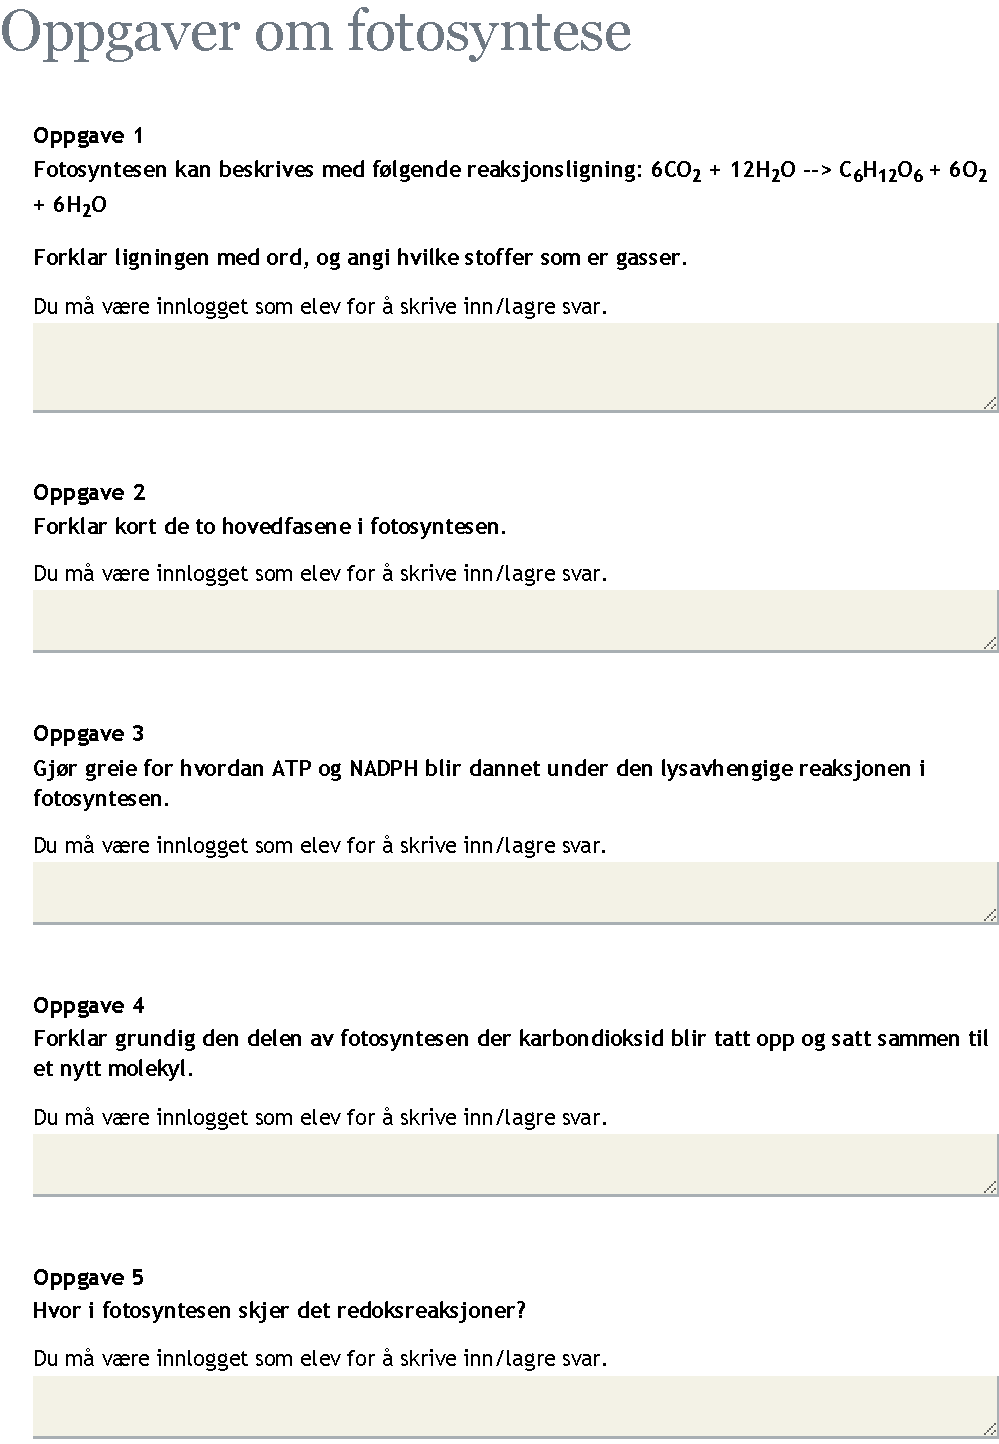
\includegraphics{img/theoretical/viten}} 
\fbox{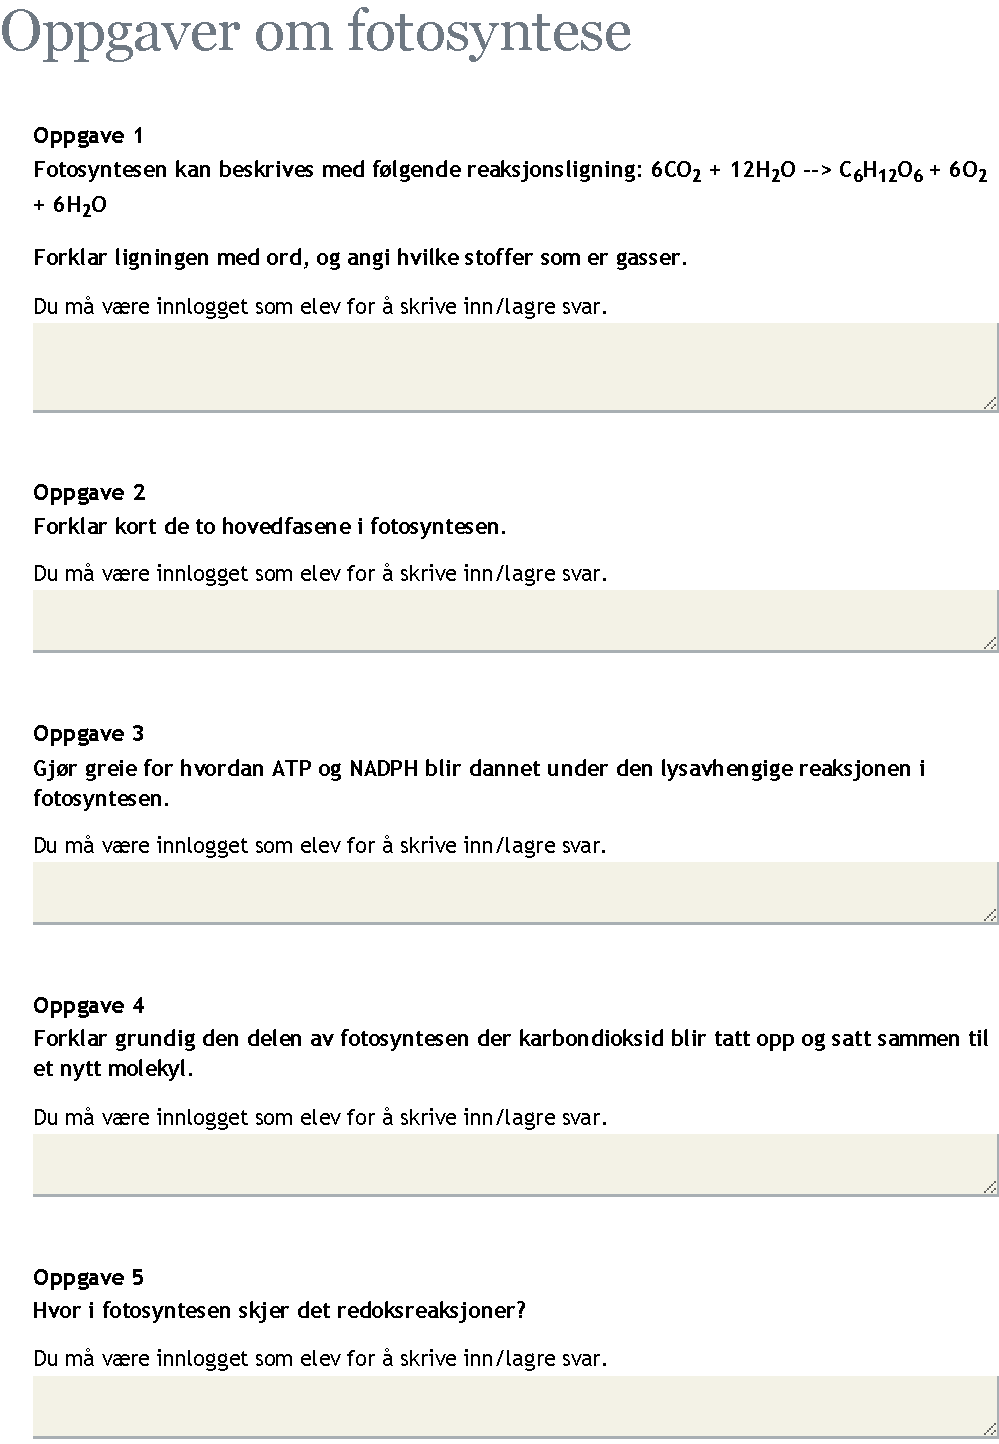
\includegraphics[width=1\textwidth]{img/theoretical/viten.pdf}}
\caption{Screenshot of viten.no showing student-role metaphor}
\label{fig:scrshotviten}
\end{figure}

Likewise \citet{jimenez2000doing} pose that "doing science" has an obstacle named "doing school". Where "doing science" refers to argumentation or dialog characterized by “construction, representation, evaluation of knowledge claims and investigative methods” \citep{jimenez2000doing}. While "doing school" refers to what actions and activities students and teachers do that instantiates rituals, routines and expectations in educational settings, e.g., review homework assignments, take lecture notes, take tests, complete lab activities etc. 

These school activities are often taken for granted by researchers, and serve as obstacles for "doing science", which tend to be a focus-area for researchers. Such research has contributed to the understanding of students' argumentation and knowledge claims, but as \citet*{furberg2008students} suggests; a more holistic view is needed to get a rich understanding of the complexity of students' meaning making. Meaning that both the dimension of "doing school" and the dimension of "doing science" needs to be taken into account. 

\subsection{Spontaneous and scientific concepts} \label{cha:spontaneous_scientific}
In the early stages of life, children learn for the most part by experience. Skills such as mastering the native language, walking, and running are learned through trial and error. This means that the knowledge of a concept is linked to the concrete experience where the concept was presented. A child who is presented with the concept of "brother" by a pointing gesture toward her brother, will at first only associate the word "brother" with that specific person. This is what \citeauthor{vygotsky2012thought} calls a \emph{spontaneous concept}.

An only child on the other hand, will be introduced to the concept of brother through other concepts. A parent can for instance say that "brothers are boys who have the same parents". The concept of brother will then be a general concept for the child, not linked to any concrete experiences, but to the concepts of "boys" and "parents". This is what \citeauthor{vygotsky2012thought} calls a \emph{scientificconcept}.

Spontaneous concepts are developed outside the conceptual framework and only linked to concrete experiences in the mind of the learner. If we presented the child having a brother with the abstract problem of a "brother's brother" \citep{vygotsky2012thought} he would become confused, as his only knowledge of the concept of brother is in situations with his own brother.

In contrast, scientific concepts are developed within a conceptual framework. They are immediately given a place within the system of concepts, i.e., explained by their relation to other concepts. As a result, the child is consciously aware and able to reflect on the concept \citep{van1998concept}. If we presented the only child with the abstract problem of a "brother's brother", he would most likely be able to solve it because of the concept's relation to other concepts in the mind of the child. 

Another example is how children develop a concept of time. In the early stages of life, a child may think that day and night is analogous to light and darkness. This is the spontaneous concept, which is saturated by experience. It is only later in life he learns the scientific concepts of the earth's rotation and its relation to the sun and the moon, which marks days and years. This information has not been appropriated by experience, as the child has not been to space and experienced it, the information is constructed using different signs linked together by the instructor. 

\begin{figure}
\centering
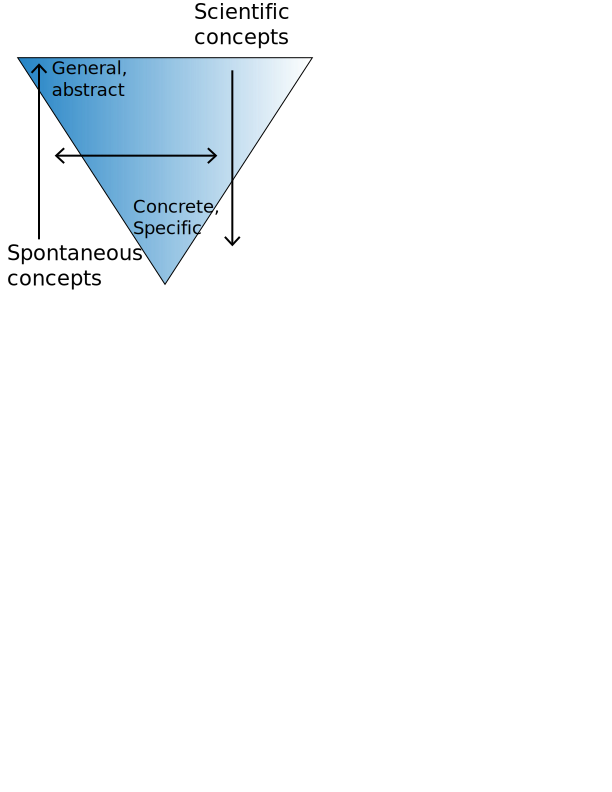
\includegraphics[width=0.6\textwidth]{img/theoretical/conceptpyramid.eps}
\caption{The concept pyramid}
\label{fig:conceptpyramid}
\end{figure}

The relationship between these two categories can be explained as an inverted pyramid. On the top we have the scientific concepts, which are general and abstract. And on the bottom we have the spontaneous concepts, which are specific and concrete. The concepts then move toward each other. The scientific concepts move downwards "toward greater concreteness" in a deductive manner, whereas the spontaneous concepts move "upward toward greater abstractness" \citep{vygotsky2012thought} in a inductive manner.

Even though the concepts move in opposite directions, there is a mutual dependency between them. In Vygotski{\u\i}'s terms: "In working its slow way upwards, an everyday concept clears a path for a scientific concept and its downward development". This means that "...the development of a spontaneous concept must have reached a certain level for the child to be able to absorb a related scientific concept" \citep[p. 194]{vygotsky2012thought}. It is therefore essential for the teacher to bring the spontaneous concepts up to a level that makes the scientific concept within reach for the student. By doing this, the student will have the experience, and the related concepts necessary for constructing knowledge of an abstract concept. 

This brings us to the zone of proximal development, as students who lack consciousness and control over the spontaneous concepts can "...find this control within the zone of proximal development" \citep[p. 194]{vygotsky2012thought}.

\subsection{Zone of proximal development}
Lev Vygotski{\u\i} was concerned with the relationship between learning and development, and argues that the theorists of his time such as Piaget, James and Koffka does not provide an adequate view of this. He finds that learning and development are interrelated, and that this relationship has some specific applications in school learning. \citep[p. 84]{vygotskiui1978mind} Thus, in order to describe these issues he introduces the concept zone of proximal development (ZPD), and defines it as follows:

\begin{quote}The distance between the actual developmental level as determined by independent problem solving and the level of potential development as determined through problem solving under adult guidance or in collaboration with more capable peers \citep[p. 86]{vygotskiui1978mind}.
\end{quote}

\begin{figure}
\centering
\includegraphics[width=0.7\textwidth]{img/theoretical/zpd.png}
\caption{The zone of proximal development \citep{wiki:zpd}}
\label{fig:zpd}
\end{figure}

The actual developmental level is in other words determined by looking at what a person can do alone. Vygotski{\u\i} found that this traditional way of determining a person's mental development does not hold in school learning, as it only describes what functions in a person that have already been matured. He therefore introduces a new developmental level, the potential development, which can describe the functions in a person that are in the process of maturation. The actual development is therefore the end product of developing, while the potential development is the state and process of developing. Teachers and instructors can then use the ZPD as a tool to delineate the immediate future of their students, i.e., their actual development of tomorrow.

Vygotski{\u\i} proposes further that ZPD is an essential feature of learning, which distinguishes learning from development, but at the same time provokes developmental processes that would not be possible without learning. In other words,

\begin{quote}It awakens a variety of internal developmental processes that are able to operate only when the child is interacting with people  in  his  environment  and  in  cooperation  with his peers \citep[p. 90]{vygotskiui1978mind}.
\end{quote}

By applying the ZPD to learning situations, the key takeaway is that the analysis alters the traditional view of knowledge or mastery, and shows that the constructed knowledge provides the basis for further development. A great example of this is the process of mastering native language, which initially is learned as a means of communication between the child and other people. The use of language first happens on a social level, in the interaction with people, and is later developed to internal speech and becomes a means to organize thought, i.e., an internal mental function. Vygotski{\u\i} calls this concept the \textit{duality of learning} \citep{vygotskiui1978mind}. 

Another classic example is that of a child trying to grasp a ball. At first the gesture means nothing to the child, but when the mother realizes that the gesture indicates something, the situation changes dramatically. When she gives him the ball, as a result of the hand gesture, the "...grasping movement changes to the act of pointing" \citep[p. 56]{vygotskiui1978mind}. This means that the operation that was initially an external activity is now "...reconstructed and begins to occur internally" \citep[p. 57]{vygotskiui1978mind}. Thus, \textit{externalization} precedes \textit{internalization}. 

With this in mind, a teacher can understand what developmental processes is maturing in their students, and from that give adapted challenges, show partial solutions and in general tailor what to say and teach next. From this perspective, development is lagging behind learning, and the challenge for the teacher becomes to teach ahead of development, but at the same time not too far ahead. This leads us to the concept of scaffolding, which can be argued to be a refinement of ZPD. 

\subsection{Scaffolding}
Vygotski{\u\i}'s zone of proximal development is the distance between what a person can do alone and what he can do with help from a more knowledgeable other (MKO). What types of help and how the MKO should provide it, has not been a focal point for Vygotski{\u\i}. Although \citeauthor*{wood1976role} does not reference to any Vygotski{\u\i}an literature, the term scaffolding introduced by them in 1976, bears resemblance to the very idea of ZPD. As they put it:

\begin{quote}Scaffolding consist essentially of the adult "controlling" those elements of the task that are initially beyond the learner’s capacity, thus permitting him to concentrate upon and complete only those elements that are within his range of competence \citep[p. 90]{wood1976role}.
\end{quote}

Thus, scaffolding can be applied by MKOs in order to keep the learning process within the learner’s ZPD. There is a is a nuanced balance for how much guiding is needed and a key point is that a person's ZPD is personal, thus a scaffold should be personally adjusted. An example can be if we were to teach two persons how to take a picture with a professional DSLR camera, one being an old woman (Mary) with little insight in technology, the other a young man (Ryan) who has grown up with technology. It is obvious that the two persons have different cultural backgrounds and taking a picture have different meanings to them, hence the tutoring of them need to be tailored differently. In the following section we will go through the six steps of scaffolding provided by \citet{wood1976role} using this example.

\begin{enumerate}
\item{} \emph{Recruitment} - We need to get the learners attention and interest in the task at hand. In our case this could be to show nice pictures of Mary's grandchildren to make her interested in taking nice pictures of them herself. For Ryan we could show the difference between pictures taken with an iPhone and a DSLR camera to make him understand the value of using a DSLR versus his iPhone.

\item{} \emph{Reduction in degrees of freedom} - The task must be narrowed down in order to provide a clear goal that can be reached. For Mary we can say that her task is to take a photo of her grandson playing in the garden with the use of auto-mode. And for Ryan, the task could be to take a landscape photo of his favorite view for his Facebook cover photo with the camera setting called A for aperture, which lets him control the depth of field - an important setting when photographing landscapes. 

\item{} \emph{Direction maintenance} - The learners must be kept on the path toward the goal, which implies a focus on motivation. Both to maintain progression and to keep a focus on the goal. From this point, scaffolding becomes an improvisation skill and it can be hard to plan ahead because of all the unforeseen things that can happen. Ryan can for example stop focusing on the landscape photo and instead take pictures of a car. While Mary starts looking at the pictures contained on the camera's memory stick. In this case one has to evaluate the goal versus the reduction in degrees of freedom. It might be that Ryan is more interested in taking pictures of cars, and since the main goal is to learn to take photos with a DSLR camera, an adjustment of the end product can be done. In Mary's case however, she might be easily distracted, and just needs someone to tell her to focus on taking pictures of her grandson. These are nuances that can be hard to spot, and requires a tutor with good improvisation skills.

\item{} \emph{Marking critical features} - Marking what the learner has done versus what is expected. This could be to show Mary that in her picture, she has left half her grandson's head out of the picture, and that she should try to capture a photo with the whole face visible. For Ryan it could be to point out that he has a very small depth of field in his photo, putting the trees in the foreground into focus, while leaving the mountains in the background blurred. Examples of correct solutions could be used to demonstrate the discrepancies between what the learner has produced and a correct solution.

\item{} \emph{Frustration control} - Balancing the dependency of the tutor and the independent problem solving. Both Mary and Ryan should be given some space to try taking photos, but we should at the same time be observant of when guiding or telling is needed. We could tell them to have the sun behind them to get the right light conditions, and hold the camera with two hands. The major risk here, is that the learner can become too dependent of the tutor, making it harder for the learner to achieve the goal, i.e., taking a picture alone at a later time.  

\item{}  \emph{Demonstration} - Showing a solution to the task, imitating the learner's earlier attempts and possibly correcting errors, with a hope that the learner will imitate back in a more correct manner. For Mary we could take a picture of her grandson, imitating her position, look for the sun, and then correct the position to get the sun behind us. Or for Ryan we could place the camera on a chair and use a timer to reduce movement of the camera, thereby allowing a slower shutter speed. This would allow a higher aperture, increasing the depth of field, giving focus to both the trees in the foreground and the mountains in the background. This might be supplemented by telling, to provide a context to the tutor's actions.
\end{enumerate}

As presented, some of these steps require planning while others require improvisation. Both the planning and improvisation turns out to be tailored to the specific situation at hand with all the complex contexts the learners bring with them to the situation. The steps can either be carried out manually by a tutor, or be mediated automatically by a computer-based system. \citet[p. 1]{fischer1991critics} presents one implementation of a computer-mediated scaffold where a critiquing system gives the user a "...reasoned opinion about a product or action generated by a human". Another example is from \citet{furberg2009socio} where prompts requiring user-input is used to promote student reflection. 

One important thing to note when reviewing the literature on scaffolding by \citet{wood1976role} and ZPD by \citet{vygotskiui1978mind} is that these studies are done on pre-school children. Critics may therefore argue that the concepts are not applicable to adult learning. Our stance is that when learning new concepts, both children and adults are alike. New and unknown concepts are new and unknown both for adults and children, and adults therefore become "as children" when introduced with new learning material. The concepts can therefore be used to analyze learning in all contexts where learning takes place. 

%Even though the six steps provided by \citet{wood1976role} can be considered as a framework for scaffolding, it is still quite complex and demands careful consideration by the teacher or the designers of the computer based scaffold.  

\section{Multiple external representations}
Multiple external representations (MER) are often used for conveying information. Textbooks and manuals contain images and illustrations, maps show different information in different ways, and whiteboards are used in addition to speech. With digital technology the possibilities of MER are expanded to include dynamic linking between the representations, and the representations can show dynamic information that is not available in the real world, e.g., visualizing the flow of oxygen. 

In an effort to identify the features of MER, \citet{ainsworth1999functions} has developed a classification framework. She suggests that MER can serve primarily three different purposes in learning situations:
\begin{enumerate}
\item{} \emph{Complementary roles} - Different representations can focus on different aspects of the phenomenon under study, or they can contain different information of the same phenomenon. E.g., a topographic map in addition to a road map. 
\item{} \emph{Constrain interpretation} - One representation can be used to constrain the interpretation of the other. E.g., the text “the fork lies next to the spoon”. It is impossible to tell which side the fork is on, but by presenting an illustration of the example, the representation will constrain the interpretation of the text. 
\item{} \emph{Construct deeper understanding} - MER can be used to "...promote abstraction, to encourage generalization and to teach the relation between representations" \citep[p. 141]{ainsworth1999functions}. 
\end{enumerate}

The three different roles presented above are also the benefits of using MER. Complementary roles can support students to make up for insufficient knowledge of one representation by using another, constrain interpretation can “support the learners’ reasoning about the less familiar representation” \citet{ainsworth1999functions}, and finally the learners can gain deeper understanding of the domain by translating between representations \citep{van2006supporting}. 

On the other hand, when learners are faced with MER they must also undertake additional tasks as to understand the phenomenon or domain in question. This may lead to a heavy cognitive load, which "...may leave less resources for actual learning" \citetext{\citealp{sweller1988cognitive,sweller1989cognitive}, referenced in \citealp{van2006supporting}, p. 200}. A key issue is then to reduce the cost for learners associated with MER, while keeping the benefits. 

\section{Inquiry learning}
According to \citet{prince2006inductive} science has traditionally been taught in a \textit{deductive} manner. In the same way as Sherlock Holmes collects piece by piece to form a theory, the students collect pieces of models and illustrations to grasp a scientific concept. Little attention is paid to why the students should learn the material, apart from having to perform on tests.

On the other hand we have the \textit{inductive} ways of teaching and learning. Instead of beginning with the theory, the students are presented with some sort of task, which becomes the motivation to learn the tools required to solve the task. Examples of this can be to make a battery in a science class, or finding out why potato-chips bags seem more inflated on the top of a mountain than by the sea.

Inquiry learning involves giving the students "...questions to be answered, problems to be solved, or a set of observations to be explained" \citep[p. 127]{prince2006inductive}, or in other words: giving the students incentives to ask for information. There are several other inductive learning methods, such as problem-based learning, discovery learning and project-based learning, which all can be explained with the same statements as inquiry learning. Inquiry learning can therefore be seen as an umbrella term for inductive learning methods. \citep{prince2006inductive}

\citeauthor*{staver1987analysis} \citetext{\citeyear{staver1987analysis}, referenced in \citealp{prince2006inductive}} differentiates between \emph{structured inquiry} (e.g., tutorials), \emph{guided inquiry} and \emph{open inquiry}. Depending on the student's developmental level, different framings of the inquiry process are needed. To scaffold the inquiry learning process is not an easy task. In a review article, \citet{de1998scientific} identifies four problems that learners may encounter when engaging with inquiry learning: \textit{hypothesis generation}, \textit{design of experiments}, \textit{interpretation of data}, and \textit{regulation of discovery learning}. They continue to argue for the need of supporting students during the process of scientific inquiry, providing scaffolds for each of these problems. The challenge then becomes to "...guide students to the "right" path, but at the
same time letting them discover and make the discovery their own" \citep[p. 247]{kluge2010simulation}. In other words the students need to be steered toward the interesting discoveries, but at the same time have the freedom to explore and not be commanded in any way.

\subsection{Misconceptions}
Misconceptions appear in most educational contexts. According to \citet[p. 437]{gomez2008elementary} students have "...qualitative differences in his or her understanding of science that is often inconsistent with what the teacher intended through his or her instruction". These are often deeply rooted, and remain intact even after instruction. This becomes especially relevant when dealing with inductive learning methods, as the students are given more freedom to explore their own ideas, and thus more freedom to pursue tracks that may lead to different conclusions than the ones intended by the instructor.

The term itself has been given many labels in research literature, depending on the focus: "alternative frameworks", "preconceptions", and "student ideas" are just some of them. An important factor here is how misconceptions are perceived. Are they resources for learning, or obstacles that the learner has to overcome? If we look at meaning making from a constructivist point of view, advanced knowledge is built upon prior understanding. Misconceptions then become "...faulty extensions of productive prior knowledge" \citep[p. 152]{smith1994misconceptions}.

To simply write misconceptions off as mistakes is, according to \citet{smith1994misconceptions}, a too narrow view in their role in learning. If we take the example of stating that "multiplication makes numbers larger", it is indeed an accurate explanation of most multiplication pieces. The problem arises in the few cases where we multiply by non-natural numbers. The conception that leads to erroneous conclusions in some contexts can be quite useful in others \citep{smith1994misconceptions}. The misconceptions are therefore for the students "...conceptions in their own right with plausibility and at explanatory power" \citetext{\citealp{smith1994misconceptions}, referenced in \citealp{larkin2012misconceptions}, p. 928}. 

%As stated before, the goal then becomes to scaffold the students in such a way that the interesting discoveries are made, and the misconceptions discussed. 

\section{Outline of concepts for analysis}
We have now introduced the sociocultural perspective and several important concepts within and besides its frames. Further we will use this perspective and the following concepts to guide our research design and discuss our findings: \emph{zone of proximal development}, \emph{scaffolding}, \emph{spontaneous and scientific concepts}, \emph{multiple external representations}, \emph{institutional practices}, \emph{inquiry learning}, and \emph{misconceptions}.

%!TEX root = ../document.tex
\chapter{Empirical settings and methods}
In this chapter...

\section{Empirical setting}
The collection of data material used in this thesis took part in the late autumn, 2013, at a high school located in the centre of Oslo. The school is in the upper third on the grade scale, with a limit of 43.5 points for admission in 2010/2011 \citep{utdanningsetaten}. Therefore the students at this school are mostly high achievers. 

Contact with the school was first initiated through Intermedia, and a presentational flyer was sent as an explanation of the project (_____appendix_____). Luckily our request coincided perfectly with a 2 week time frame for reviewing photosynthesis in one of the teacher's classes, and he was therefore quite eager to use our application in class. 

The class selected for the experiment was a biology class at the highest level offered at the school, biologi 2, which has an extensive curriculum covering e.g photosynthesis, enzymes and energy transmitters. The students were between 17 and 18 years of age, and for the main part most of the 20 students taking the class were present. All the students aggred to participate in the study, but due to technical limitations, data collection was only done with a small sample of the group. 


\def\arraystretch{1.8}
\begin{table}
    \begin{tabular}{@{}lp{250pt}@{}}\toprule
    Sensor               & Description \\ \midrule                                                                                                  
    TSL2561              & Digital luminosity sensor. Measures light in lux from 300-1100nm.                                            \\ 
    RHT03                & Digital humidity and temperature sensor. Measures relative humidity and temperature in celsius.              \\ 
    DS18B20              & Digital waterproof temperature sensor. Measures temperature in celsius                                       \\ 
    DFRobot sku:sen0114  & Analog soil moisture sensor. Returns values between 0 and 900 depending on electrical conductivity of soil.  \\ \bottomrule
    \end{tabular}
    \caption{Sensors used in the application}
\end{table}


With the advent of the \emph{“internet of things”}, sensors are becoming available in many different forms and packages. Just as LEGO-pieces they can be used in a wide range of applications. From automating tasks such as keeping a steady indoor-temperature, to measuring variables which we as humans cannot see. 

For this application we did a short review of the available off-the-shelf packages available on the market. 

The sensors are able to capture information about the environment and transform it to data variables which we can store and categorize. In total there are five different sensors connected to the plant, or in the plant’s vicinity: soil moisture, soil temperature, air temperature, humidity, and light. 


(write something about the sensortag)

Simplified we can say that the sensors function in the same way as a volume controller on an amplifier. On an amplifier one can adjust the volume by varying the resistance in the signal going to the speakers. If we turn the volume up, the resistance goes down, which lets more power through to the speakers. And if we turn the volume down, the resistance goes up which lets less power flow to the speakers. The concept with sensors is the same, only that instead controlling resistance with a volume knob, it is controlled by light, moisture or other environmental variables. 

For a good example, lets look at how the temperature sensors work. The resistors used in the temperature sensors are called “thermistors”, and the way they operate is by varying the resistance according to the temperature. Since we already know how many volts we are sending to the thermistor on the one end, we can use the amount of volts we get back to calculate the resistance. In our application this is done by a voltage divider which uses a formula as follows: 

\begin{equation}
U_{out}=\frac{R_{2}}{R_{1}+R_{2}}\cdot U_{in} 
\label{eq:vdiv1}
\end{equation}
Where $V_{out}$ is voltage out, $U_{in}$ is voltage in, $R_{1}$ is a given resistance, and $R_{2}$ is the resistance we want to calculate. For this example let's assume that $U_{in} = 5_{v}$, $U_{out} = 2_{v}$, and $R_{1} = 1K\Omega$. We solve this equation with regard to $R_{2}$
\begin{equation}
R_{2} = \frac{U_{out} \cdot R_{1}}{U_{in}-U_{out}}
\end{equation} 

\begin{equation}
R_{2} = \frac{2V \cdot 1000\Omega}{5V-2V}
\end{equation} 

\begin{equation}
R_{2} = \frac{2000\Omega}{3}
\end{equation} 

\begin{equation}
R_{2} = 667\Omega
\end{equation} 

Then we can see that the calculated resistance is 667$\Omega$. This value can then be mapped to the correct unit of measure, in this case Celsius or Fahrenheit. 

As we are using digital sensors, all of these calculations are done internally in the sensors, and coded into a digital signal. This signal, consisting of 1s and 0s, is then passed onto the next unit in our system, the Arduino.  

\subsection{Arduino}
(Write about embedded systems. What other alternatives are there to the Arduino? )

Arduino is an open-source prototyping platform which makes it easy to interface low-level electronics (e.g sensors) with higher-level electronics (e.g computers). The core part of the Arduino is an Atmel\texttrademark Atmega microcontroller which can be programmed by a computer over usb, using the Arduino programming language and the Arduino development environment \citep{arduino}.

We have used an Arduino Uno which has 13 digital input output pins (GPIO), five analog inputs, i2c inputs, and USB for serial communication. The DSB18B20 soil temperature sensor and RHT03 temperature and humidity sensor are connected to the digital inputs through a 1K(ohm) pullup resistor. The pullup resistors are used to keep the voltage sent to the arduino from fluctuating when the sensor is not sending any data. The TSL2561 luminosity sensor is connected to the A4/SDA and A5/SDL ports of the Arduino as it communicates over the i2c protocol. And the DFRobot soil moisture sensor is connected to A3 (Analog input 3) as it outputs analog voltage.  

\begin{figure}
\centering
\includegraphics[width=1\textwidth]{img/hardware/Arduino_and_sensors_schem.png}
\caption{Schema diagram of Arduino sensor wiring}
\label{fig:arduino}
\end{figure}

The community surrounding Arduino is quite large, and therefore we were able to find pre-written libraries for communicating with the different sensors. This has made the task of converting the digital signal to the correct units (celsius, relative humidity, lux) and levels a breeze. 

In the case of the soil moisture sensor, it does not output soil moisture in any kind of universal unit. Therefore we measured the resistance in air (high resistance), and in water (low resistance), and let these be the high and low points of a new unit called arbitrary moisture units (AMU).

The code residing in the arduino runs a simple loop where it waits for a special character sent over serial communication through USB. If it receives this character it reads all the sensor values, and sends them back to the next logical unit: the Raspberry Pi

\subsection{Raspberry Pi}
(Why raspberry? Beagleboard?)
The Raspberry Pi is a “cheap, accessible, programmable computer” \citep{raspberrypi} which is roughly the size of a credit card. Our model was released early 2012, and contains two usb ports, audio, sd-card slot, and several GPIO-pins. The devices connected to it are: wireless network adapter, high-definition webcamera, and the Arduino. The operating system running on it is a port of Debian Linux optimized for the Raspberry, called Raspbian. 

(illustration of raspberry)

The GPIO-pins on the raspberry works almost in the same fashion as the Arduino’s digital input output pins. Thus we could in theory simplified the hardware by omitting the Arduino. The main reason for not doing this is that the Raspberry does not have an analog to digital converter (ADC). Therefore we would have to make a complex circuit involving an ADC to interface the Raspberry with the soil moisture sensor. In addition, we would most likely face timing issues. When we ask the digital sensors for data, they send the response immediately. If the unit receiving is not available to read the data, it gets lost. This can be a problem when using a high-level computer, as it performs multiple other tasks in addition to reading sensordata. 

\subsubsection{Operation}
After booting up an endless loop bash-script is called. The script snaps a photo of the plant using the webcam, and then runs a python-script responsible for collecting sensordata. Since we sometimes can get erroneous values from the sensors, we read 15 values and upload the median value.

%http://en.wikibooks.org/wiki/LaTeX/Packages/Listings
\lstset{language=Python} 
\begin{figure}
\begin{lstlisting}
//instantiate lists
airtemp = []
humidity = []
light = []
soiltemp = [] 

for x in xrange(1,15): 
	ser.write("r") //Ask Arduino for data
	variables = ser.readline() //Read the data
	sensorReadings = variables.split('|') //Split string on |

	airtemp.append(float(sensorReadings[0]))
	humidity.append(float(sensorReadings[1]))
	light.append(float(sensorReadings[2]))
	soiltemp.append(float((sensorReadings[3])[:-2])) 

//calculate and post the median using numpy
postData(np.median(airtemp),np.median(humidity),np.median(light),np.median(soiltemp)) 
\end{lstlisting}
\caption{Reading sensor values from Arduino on Raspberry PI}
\label{fig:raspberrycode}
\end{figure}

These values, along with the photo of the plant, are then passed on to the next instance, the API, using pythons HTTP-library urllib2. 

\section{Data processing and database}
When the data has been gathered at the low level hierarchy, it is stored in the cloud. This is done by posting the data to an API on our web server. The main function of an API is to be a mean of communication between software, in our case the data collector and the user interface. After some research on web-API design, we decided that a REST architectual style was the way to go. 

\subsection{Representational State Transfer (REST)}
REST is an architectual style for distributed hypermedia systems \citep{fielding2000architectural}. In Fielding's dissertation, he writes about the interaction constraints of REST that is introduced in order to limit how a distributed system can be constructed. 
=======
\subsection{Planning}
The planning of the project was done by us in conjuction with the teacher responsible for the for the biology class. An initial plannign meeting was held at the school around one week before the experiments started. There we gave the teacher a thorough introduction of the system, and presented some ideas for expirements the students could perform using our system as platform. This involved:
>>>>>>> 4056fd08d59c7d41cdee9e1f90c94e5ae23dbd4d

\begin{enumerate}
\item{Present the application in class}
\item{Initiate an experiment using the application. Related to e.g soil moisture, light intensity, light quality, or temperature}
\item{Have a one hour session where the students work with text tasks realted to the experiment}
\end{enumerate}

The teacher then suggested that we could conduct two experiments, so the students could work on the relations between the different external factors effect on photosynthesis. As the system records a range of different variables, it would be possible to keep the environment relatively controlled, or at least point to factors which could be sources of error in the experiment. 

We agreed that the factor where we could get the most interesting result was to vary the light intesity and the light quality (wavelength). The first experiment would then involve keeping the plant located in a window facing west, receiving sunlight and light from the fluorescent indoor-lighting. In the second experiment we would plant new seeds, and relocate the plant to a (presumably) light proof cupboard. The plant would then only be given green light, with a known wavelength. Each of the experiments would have a duration of approximately one week. 

\subsection{Execution pow pow ?}
The project was presented and the first experiment initiated by one of the students on friday 25th of october. This went on until friday 1st of november when the second experiment was initiated. The second experiment went on until wednesday 13th of november when the primary data collection session started. During the experiments we were present at four separate occations, observing what the teacher was focusing on, and what kind of questions/which part of the photosynthesis the students found most difficult. In addition to answering questions about the system, and if/how the system was used in the education. 

\subsection{Data collection}


Our main data material consists of x hours of video from the session... blabla

\section{Analytical Procedures}

\subsection{Ethics}




%!TEX root = ../document.tex
\chapter{Data \& Analysis}
In this chapter we will present the findings from our case study ...

\section{Hypothesis generation}

\subsection{Context}
In table~\ref{excerpt:expectations1} the students are discussing assignment 1a, and are talking about what they thought would happen to the plant which only got green light. While discussing they are also describing the what the conditions for the plant was. The plant from the closet is in front of them on the table, but they do not know which plant it is. 
\subsection{Raw data}


\def\arraystretch{1.5}
\begin{table}
\begin{adjustwidth}{-4em}{-4em}
\begin{center}
\begin{tabular}{r l p{9cm} p{4cm} } \toprule
	Time &  Who &  Speech  & Action\\ \midrule  

	2:16 %time
	&Siri %name
	&\parbox[t]{9cm}{\raggedright .. det var det planten stod i skapet også skulle det være bare grønt lys på den ... men det kan jo hende for eksempel at det kom litt annet lys inn i skapet også .. så da er det ikke sikkert at det bare bar grønt lys ..  %speech 
	}&\parbox[t]{4cm}{\raggedright peker på skapet %action 
	}\\

	2:31 %time
	&Nora %name
	&\parbox[t]{9cm}{\raggedright  %speech 
	}&\parbox[t]{4cm}{\raggedright nikker %action 
	}\\

	2:31 %time
	&Siri %name
	&\parbox[t]{9cm}{\raggedright og planten tar jo opp littegrann grønt lys også, men ikke så mye .. så derfor kunne det hende atte den ikke vokste like my.. eller jeg trodde at den ikke ville vokse like mye i skapet .. siden da fikk den bare grønt lys ...  %speech 
	}&\parbox[t]{4cm}{\raggedright  %action 
	}\\

	2:46 %time
	&Nora %name
	&\parbox[t]{9cm}{\raggedright ... mmm ... %speech 
	}&\parbox[t]{4cm}{\raggedright  %action 
	}\\

	2:47 %time
	&Siri %name
	&\parbox[t]{9cm}{\raggedright eller neste bare grønt lys ihvertfall ... men hvor mye vokste den egentlig? er det den ((refererer til planten på bordet)) som stod i skapet? %speech 
	}&\parbox[t]{4cm}{\raggedright peker på planten som står på pulten %action 
	}\\

	2:52 %time
	&Sjur %name
	&\parbox[t]{9cm}{\raggedright ja %speech 
	}&\parbox[t]{4cm}{\raggedright  %action 
	}\\

	2:53 %time
	&Nora %name
	&\parbox[t]{9cm}{\raggedright OJ(!) %speech 
	}&\parbox[t]{4cm}{\raggedright  %action 
	}\\

	2:53 %time
	&Siri %name
	&\parbox[t]{9cm}{\raggedright Den har jo vokst ganske mye %speech 
	}&\parbox[t]{4cm}{\raggedright smiler %action 
	}\\
	
	\bottomrule
\end{tabular}
\end{center}
\end{adjustwidth}
\caption{Excerpt from exercise 1}
\label{excerpt:expectations1}
\end{table}

\subsection{Explanation}
Siri had an expectation that the plant from the closet would not grow as much as the plant from the window, and she is explaining why she thinks that. At the same time, she knows from looking at the system earlier, that the plant have grown, so she tries to explain why it has grown at all. 


\section{Hypothesis generation}

\subsection{Context}
After looking at the plant on the table the student wanted to know if the stems on the plants in the window where white as the stems in the closet. They opened monoplant and navigated to the videolist, where they got an overview over the looks of the two different plants. They checked the color of the stems, and opened a video from 31th of October, then pressing play. This is when Fredrik starts to talk in table~\ref{excerpt:hypothesis1}.



\subsection{Raw data}


\def\arraystretch{1.5}
\begin{table}
\begin{adjustwidth}{-4em}{-4em}
\begin{center}
\begin{tabular}{r l p{9cm} p{4cm} } \toprule
	Time &  Who &  Speech  & Action\\ \midrule  

	3:24 %time
	&Fredrik %name
	&\parbox[t]{9cm}{\raggedright mhm ... mmja så da er det jo egentlig ganske ... ja ikke så stor forskjell da på de som stod ...  i skapet ((peker på planten på border)) og de som stod i vinduskarmen hvis man bare ser på ...  utseende %speech 
	}&\parbox[t]{4cm}{\raggedright Dette sies mens Siri starter videoen, hun stopper også videoen før de har sett den halvferdig. %action 
	}\\

	3:37 %time
	&Siri %name
	&\parbox[t]{9cm}{\raggedright ja .. men da ville jeg kanskje tenke at det kan hende at det kom inn annet lys enn det grønne lyset også. siden de har vokst så bra, og at de vokser bedre hvis de får flere.. lys i flere bølgelengder enn bare grønt lys %speech 
	}&\parbox[t]{4cm}{\raggedright Stemmeleiet går opp mot slutten av setningen, og løfter blikket fra arket for å få bekreftelse %action 
	}\\

	... %time
	&... %name
	&\parbox[t]{9cm}{\raggedright \emph{Intervensjon hvor Sjur introduserer og forklarer bildet av lysspekteret på oppgavearket.} %speech 
	}&\parbox[t]{4cm}{\raggedright  %action 
	}\\

	4:14 %time
	&Siri %name
	&\parbox[t]{9cm}{\raggedright mhm ... der er det jo litt blått lys og sånt også. %speech 
	}&\parbox[t]{4cm}{\raggedright Peker på det blå lyset i illustrasjonen øverst på oppgavearket %action 
	}\\

	4:18 %time
	&Nora %name
	&\parbox[t]{9cm}{\raggedright ja så det er ikke bare rent grønt … %speech 
	}&\parbox[t]{4cm}{\raggedright  %action 
	}\\

	4:20 %time
	&Fredrik %name
	&\parbox[t]{9cm}{\raggedright ... ja det er jo ikke bare på 500 circa ((referer til bølgelengde)), det er jo et stort område %speech 
	}&\parbox[t]{4cm}{\raggedright Holder hendene fra hverandre som om han signaliserer hvor langt noe er. %action 
	}\\

	4:26 %time
	&Siri %name
	&\parbox[t]{9cm}{\raggedright mhm, og planten tar jo ihvertfall opp veldig mye blå .. blårlilla lys ... %speech 
	}&\parbox[t]{4cm}{\raggedright  %action 
	}\\

	4:31 %time
	&Fredrik %name
	&\parbox[t]{9cm}{\raggedright ... mhm ... %speech 
	}&\parbox[t]{4cm}{\raggedright  %action 
	}\\

	4:32 %time
	&Siri %name
	&\parbox[t]{9cm}{\raggedright så da har den sikkert kunnet utnytte mye av dette her. %speech 
	}&\parbox[t]{4cm}{\raggedright peker på det blå spekteret i illustrasjonen øverst på oppgavearket %action 
	}\\


	\bottomrule
\end{tabular}
\end{center}
\end{adjustwidth}
\caption{Excerpt from hypothesis generation 1}
\label{excerpt:hypothesis1}
\end{table}

\subsection{Explanation}
Fredriks observation on the appearance of the plants breaks Siris expectation that the plant in the closet would not grow as much as the on in the window. Siri starts to explain why this could have happened by talking about light in different wavelengths, but without explaining why this has any effect on growth, only stating that it has an effect.
Sjur drops in and introduces the illustration of the green light on the paper as it appears as if they have not seen this yet. This gives the students more hold in Siris explanation that it might not only be green light in the closet, as the green lamp produces some light in the blue specter. So they now have two possible explanations to why the plants have grown (in their eyes) the same amount. Firstly, there might have been some light pollution coming into the closet, and secondly the green light is not purely green.

\section{Hypothesis generation}

\subsection{Context}
In table~\ref{excerpt:disconfirmation1} the students have been looking at the movements of the two plants, and have observed that the plant in the window are moving towards the sun, a so called heliotropism. They are now observing that the plant in the closet is just growing straight up without any large movement like the other plant. Suddenly Nora observes that the plant is growing a lot more than the window plant.
\subsection{Raw data}


\def\arraystretch{1.5}
\begin{table}
\begin{adjustwidth}{-4em}{-4em}
\begin{center}
\begin{tabular}{r l p{9cm} p{4cm} } \toprule
	Time &  Who &  Speech  & Action\\ \midrule  

	7:46 %time
	&Nora %name
	&\parbox[t]{9cm}{\raggedright Jeg føler at de vokser veldig mye inni ... skapet eller er det? ... %speech 
	}&\parbox[t]{4cm}{\raggedright  %action 
	}\\

	7:51 %time
	&Siri %name
	&\parbox[t]{9cm}{\raggedright Ja det virka som om de vokste ... %speech 
	}&\parbox[t]{4cm}{\raggedright  %action 
	}\\

	7:53 %time
	&Nora %name
	&\parbox[t]{9cm}{\raggedright ... ser ut som de ble lenger lissom ... %speech 
	}&\parbox[t]{4cm}{\raggedright  %action 
	}\\

	7:53 %time
	&Siri %name
	&\parbox[t]{9cm}{\raggedright ... enda mer der. %speech 
	}&\parbox[t]{4cm}{\raggedright  %action 
	}\\

	7:54 %time
	&Fredrik %name
	&\parbox[t]{9cm}{\raggedright ja %speech 
	}&\parbox[t]{4cm}{\raggedright  %action 
	}\\

	7:56 %time
	&Siri %name
	&\parbox[t]{9cm}{\raggedright ... enn ute, at de ble mye lengre. %speech 
	}&\parbox[t]{4cm}{\raggedright  %action 
	}\\

	7:59 %time
	&Fredrik %name
	&\parbox[t]{9cm}{\raggedright mhm. %speech 
	}&\parbox[t]{4cm}{\raggedright  %action 
	}\\

	8:01 %time
	&Siri %name
	&\parbox[t]{9cm}{\raggedright Kanskje de fokuserer veldig på å vokse oppover når lyset er rett over dem.. at de vokser rett oppover ((fører hånden oppover)) i stedet for å følge lyset og gå lissom sånn sakte oppover ((snurrer hånden sakte oppover)) %speech 
	}&\parbox[t]{4cm}{\raggedright  %action 
	}\\
	
	
	\bottomrule
\end{tabular}
\end{center}
\end{adjustwidth}
\caption{Excerpt from disconfirmation of growth}
\label{excerpt:disconfirmation1}
\end{table}

\subsection{Explanation}
Siri starts at once to generate a hypothesis for why the plant in the closet are growing more than the one in the window. \sout{It might be because it is hard for her to realize that her expectations where wrong and she is trying to cope with her misconception of plants growing in green light.} Basically what she is saying is that heliotropism makes the plant in the window grow slower because it has to move after the sun, and since the plant in the closet can grow straight up, it can grow faster. 

\section{Hypothesis generation}

\subsection{Context}
Morten has asked if the students has looked at the graphs below the video, and the students have in response looked into the graphs and observed that the light graph is really different in the two enviroments. In  table~\ref{excerpt:hypothesis2} Sjur then asks the question they wondered about earlier again to see if the graphs can help them test their hypothesis. 

\subsection{Raw data}

\def\arraystretch{1.5}
\begin{table}
\begin{adjustwidth}{-4em}{-4em}
\begin{center}
\begin{tabular}{r l p{9cm} p{4cm} } \toprule
	Time &  Who &  Speech  & Action\\ \midrule  

	9:21 %time
	&Sjur %name
	&\parbox[t]{9cm}{\raggedright Men hvorfor tror dere den i skapet strekker seg så mye, den som fikk grønt lys ... %speech 
	}&\parbox[t]{4cm}{\raggedright Nora snur seg mot Sjur som står bak gruppen %action 
	}\\

	9:26 %time
	&Nora %name
	&\parbox[t]{9cm}{\raggedright De skal jo bare vokse oppover da, eller den vokser bare oppover så.. %speech 
	}&\parbox[t]{4cm}{\raggedright Siri snur seg også %action 
	}\\

	9:30 %time
	&Sjur %name
	&\parbox[t]{9cm}{\raggedright ja? %speech 
	}&\parbox[t]{4cm}{\raggedright  %action 
	}\\

	9:31 %time
	&Nora %name
	&\parbox[t]{9cm}{\raggedright Da.. har den mye energi til det? %speech 
	}&\parbox[t]{4cm}{\raggedright  %action 
	}\\

	9:33 %time
	&Siri %name
	&\parbox[t]{9cm}{\raggedright Ja kanskje den fokuserer på å vokse rett oppover ((tar hånden oppover)) når lyset står der hele tiden.. åja! også om natta så er det jo ikke sol, så da … %speech 
	}&\parbox[t]{4cm}{\raggedright  %action 
	}\\

	9:43 %time
	&Nora %name
	&\parbox[t]{9cm}{\raggedright Da vokser den jo ikke opp... %speech 
	}&\parbox[t]{4cm}{\raggedright ser usikkert mot sjur etterhvert %action 
	}\\

	9:44 %time
	&Fredrik %name
	&\parbox[t]{9cm}{\raggedright mhm %speech 
	}&\parbox[t]{4cm}{\raggedright  %action 
	}\\

	9:45 %time
	&Siri %name
	&\parbox[t]{9cm}{\raggedright da vokser den ikke etter lyset på en måte %speech 
	}&\parbox[t]{4cm}{\raggedright litt usikker i stemmen %action 
	}\\

	9:47 %time
	&Nora %name
	&\parbox[t]{9cm}{\raggedright Ja altså den vokste jo dag og natt .. i .. skapet %speech 
	}&\parbox[t]{4cm}{\raggedright  %action 
	}\\

	9:50 %time
	&Siri %name
	&\parbox[t]{9cm}{\raggedright mhm, for det var lys der hele tiden ... så den strakk seg hele tiden etter lyset %speech 
	}&\parbox[t]{4cm}{\raggedright  %action 
	}\\

	\bottomrule
\end{tabular}
\end{center}
\end{adjustwidth}
\caption{Excerpt from hypothesis 2}
\label{excerpt:hypothesis2}
\end{table}

\subsection{Explanation}
Here they found that since the plant in the closet got light all night and all day, it got more light than the plant in the window which got light only during the day.

\section{Hypothesis generation}

\subsection{Context}
Earlier Morten explicitly told the group to look at the light graphs again, however, the group only stated the fact that the window plant got a lot of light during the day, but nothing at night, where as the plant in the closet got a constant amount of light.
table~\ref{excerpt:hypothesis2} 

\subsection{Raw data}

\def\arraystretch{1.5}
\begin{table}
\begin{adjustwidth}{-4em}{-4em}
\begin{center}
\begin{tabular}{r l p{9cm} p{4cm} } \toprule
	Time &  Who &  Speech  & Action\\ \midrule  

	10:49 %time
	&Sjur %name
	&\parbox[t]{9cm}{\raggedright mens den andre gjerne .. nesten ligge på null heile veien da .. (?) %speech 
	}&\parbox[t]{4cm}{\raggedright Fredrik og Nora snur seg. Nora nikker %action 
	}\\

	10:53 %time
	&Siri %name
	&\parbox[t]{9cm}{\raggedright Å ja! det var jo lavere lys der, men så blir det veldig mye lys her når det først er lys. %speech 
	}&\parbox[t]{4cm}{\raggedright har et ganske bekymret ansiktsuttryk mens hun prøver å forstå hva hun sier. %action 
	}\\

	11:11 %time
	&Sjur %name
	&\parbox[t]{9cm}{\raggedright Men hvis dere ser på baksiden av det oppgavearket %speech 
	}&\parbox[t]{4cm}{\raggedright Peker mot arket. Nora snur arket %action 
	}\\

	 %time
	& %name
	&\parbox[t]{9cm}{\raggedright  %speech 
	}&\parbox[t]{4cm}{\raggedright  %action 
	}\\

	 %time
	& %name
	&\parbox[t]{9cm}{\raggedright  %speech 
	}&\parbox[t]{4cm}{\raggedright Lærer kommer bort %action 
	}\\

	11:20 %time
	&Lærer %name
	&\parbox[t]{9cm}{\raggedright Går det bra eller %speech 
	}&\parbox[t]{4cm}{\raggedright kommer bort til bordet og lener seg på det. %action 
	}\\

	11:23 %time
	&Siri %name
	&\parbox[t]{9cm}{\raggedright mmm, ja %speech 
	}&\parbox[t]{4cm}{\raggedright  %action 
	}\\

	11:24 %time
	&Lærer %name
	&\parbox[t]{9cm}{\raggedright skjønner dere ... har dere funnet forklaring på alle spørsmålene? %speech 
	}&\parbox[t]{4cm}{\raggedright  %action 
	}\\

	11:26 %time
	&Alle jentene %name
	&\parbox[t]{9cm}{\raggedright *** vi prøver ... %speech 
	}&\parbox[t]{4cm}{\raggedright snakker i munnen på hverandre %action 
	}\\

	11:27 %time
	&Siri %name
	&\parbox[t]{9cm}{\raggedright Jeg tror kanskje jeg har en ide om det med at den her ute ((peker mot vinduet, refererer til planten i vinduet)) ikke vokser like høyt, eller så fort ihvertfall.. fordi atte når det kommer veldig mye sol så blir jo klorofyllmolekylene eksitert, men når alle ... alle klorofyllene blir eksitert i planten, sånn atte det ikke er flere som kan bli eksitert så hjelper det ikke om det er mere lys. %speech 
	}&\parbox[t]{4cm}{\raggedright  %action 
	}\\

	11:55 %time
	&Lærer %name
	&\parbox[t]{9cm}{\raggedright Så det du tenker er rett og slett at den hemmes av for mye lys, at den ikke vokser så mye fordi det er så mye lys? %speech 
	}&\parbox[t]{4cm}{\raggedright  %action 
	}\\

	12:03 %time
	&Siri %name
	&\parbox[t]{9cm}{\raggedright Kanskje ikke hemmes .. det .. hvis det er veldig sterkt lys kan jo pigmentene bli svidd, men  når det er  litt mere lys enn alt det de kan ta opp.. så hjelper det ikke at det er litt mer, for da kan de ikke ta opp det ekstr... %speech 
	}&\parbox[t]{4cm}{\raggedright  %action 
	}\\

	\bottomrule
\end{tabular}
\end{center}
\end{adjustwidth}
\caption{Excerpt from hypothesis 2}
\label{excerpt:hypothesis2}
\end{table}

\subsection{Explanation}
In the excerpt in table~\ref{excerpt:hypothesis2} Siri understands that it is a difference in the light intensity, not just when the plants get light. However, it seems like she interprets it to mean that the plant in the window get too much light, and that light becomes a limiting factor for the plants growth. When she explains her hypothesis to the teacher later in the excerpt, she is using a more scientific language than before, and mentions chlorophyll molecules that gets excited. This might be because right before this she is introduced to the representation of the light dependent reaction of the photosynthesis, \sout{or it might be because this is the first the teacher is listening to the group}.


\section{Hypothesis generation}

\subsection{Context}

table~\ref{excerpt:scaffold1} 

\subsection{Raw data}

\def\arraystretch{1.5}
\begin{table}
\begin{adjustwidth}{-4em}{-4em}
\begin{center}
\begin{tabular}{r l p{9cm} p{4cm} } \toprule
	Time &  Who &  Speech  & Action\\ \midrule  

	13:33 %time
	&Siri %name
	&\parbox[t]{9cm}{\raggedright nei, men ... hvis de bare hadde fått grønt lys i eh den bølgelengden som de tar opp minst av så hadde kanskje planten vokst veldig lite %speech 
	}&\parbox[t]{4cm}{\raggedright  %action 
	}\\

	13:44 %time
	&Lærer %name
	&\parbox[t]{9cm}{\raggedright ja.. så altså dere tenker at .. sammenhengen mellom vekst og fotosyntese den er helt klar ... du kan ikke du tenker at du kan ik et frø kan ikke spire og vokse og bli en plante uten at drives fotosyntese.. tenker dere alle det? %speech 
	}&\parbox[t]{4cm}{\raggedright  %action 
	}\\

	14:00 %time
	&Fredrik %name
	&\parbox[t]{9cm}{\raggedright Det er jo noen planter som ikke har fotosyntese ... og de spirer jo og fordet ikkesant.. det er vel en liten energipakke på en måte i  frøet da? er det ikke det da? %speech 
	}&\parbox[t]{4cm}{\raggedright  %action 
	}\\

	14:14 %time
	&Lærer %name
	&\parbox[t]{9cm}{\raggedright okei, er det? %speech 
	}&\parbox[t]{4cm}{\raggedright  %action 
	}\\

	14:14 %time
	&Nora %name
	&\parbox[t]{9cm}{\raggedright Ja %speech 
	}&\parbox[t]{4cm}{\raggedright nikker annerkjennende %action 
	}\\
	
	\bottomrule
\end{tabular}
\end{center}
\end{adjustwidth}
\caption{Excerpt from teacher talk}
\label{excerpt:scaffold1}
\end{table}

\subsection{Explanation}
In the excerpt in table~\ref{excerpt:scaffold1} 
\section{Hypothesis testing}

\subsection{Context}
\subsection{Raw data}
\subsection{Explanation}

\section{Questions}

\subsection{Context}
\subsection{Raw data}
\subsection{Explanation}
%!TEX root = ../document.tex
\chapter{Discussion}
In this chapter we will discuss our research questions by contextualizing our findings to the theoretical concepts introduced earlier. As an overall theme we will look at the inquiry process of the students in interaction with Monoplant. This will be showed through 4 sections, the first being about the inquiry process. Next we will discuss how multiple external representations support the inquiry process of the students, then how scaffolding is instantiated in the environment, and finally how the institutional setting frame the students' inquiry process.


\section{Inquiry process}
In the previous chapter we presented excerpts from the session where the students interacted with Monoplant. We have seen that the students were generating hypotheses of what happened with the plant and why it grew as much as it did. We showed examples of explanations, discussion, misconceptions and surprises. In this section we will discuss some of these examples further and broadly address our first research question: \emph{"What characterizes the students’ inquiry in interaction with Monoplant?"}

\subsection{Tentative hypothesis}
We designed the experiments together with the teacher. The students were given a problem in form of the assignments they discussed. They had to figure out the answers with the help of Monoplant, which presented detailed data logging of the experiments. The experiments conducted combined with the problem solving-session with the students can be categorized as a hybrid of \emph{guided inquiry} and \emph{structured inquiry} \citetext{\citet{staver1987analysis}, referenced in \citealp{prince2006inductive}} as the students are given a problem and the means (Monoplant) to solve it. It is a structured inquiry in that Monoplant provides information that the students can use while solving the tasks. At the same time this information needs to be interpreted and evaluated, hence the students need to figure out how to interpret the information, making the inquiry process look more like guided inquiry.

As showed in \emph{excerpt 1}, Siri presented a hypothesis in which she stated that plant B would not grow much because it would not get as much light as plant A. In \emph{excerpt 2} data was presented to her that showed that plant B had indeed grown much. As she had already made a hypothesis, her interpretation of the data was directed by her preconceptions. Since the data disproved her first hypothesis, the next hypothesis is claiming there might be some sources of error in the experiment. Hence she is misinterpreting the data, which lays the basis for a denial of the fact that her first hypothesis was wrong, or in other words: she starts to explain why the first hypothesis did not hold even though she still thinks it should.

\citet{de1998scientific} addressed four problems that students encounter during inquiry learning. These were classified according to the main discovery learning processes: \textit{hypothesis generation}, \textit{design of experiments}, \textit{interpretation of data}, and \textit{regulation of discovery learning}. In our case we controlled two of these stages by designing and initiating the experiments for the students, as well as letting Monoplant do a systematic logging of data during the experiment, hence regulating the inquiry process. This meant that the students were facing two of the stages: interpreting the data and generating hypotheses based on their interpretation of the data. These two are closely linked and mutually dependent. \citeauthor*{klahr1993heuristics} \citetext{\citeyear{klahr1993heuristics}, referenced in \citealp{de1998scientific}} reported that misinterpretation of data often result in confirmation of the current hypothesis. In the case with Siri in \emph{excerpt 1} and \emph{2}, we can see that she is sticking to her first hypothesis when interpreting new data, but she tries to make the experiment invalid as the data compromise her understanding. \citeauthor*{dunbar1993concept} \citetext{\citeyear{dunbar1993concept}, referenced in \citealp{de1998scientific}} have also found evidence of the tendencies for students to keep initial hypothesis rather than stating a new. He mentions what calls the "unable-to-think-of-an-alternative-hypothesis" phenomenon, as a possible explanation. This means that the students keep their current hypothesis (despite conflicting evidence) simply because they have no alternative.

\subsection{Delayed inquiry}
The students were done with the textbook chapter of photosynthesis and were able to explain  phenomena such as growth theoretically. Their presumptions to the outcomes of the experiment colored their interpretation of data because it was connected to the students' prior conceptual knowledge. Siri knew that plants make food for themselves by doing photosynthesis. To do photosynthesis, a green plant such as the cress in the experiment, needs light of wavelengths other than green (e.g blue and red). This reasoning makes sense to Siri because she knows a lot about the scientific concepts concerning the theme at hand. We can say that the inquiry process became deductive as it was affected by the students preconceptions and their ability to explain the observations they made with Monoplant. 

However, this is a misconception in inquiry learning, and what \citet{gomez2008elementary} refers to as \emph{inconsistent understanding}, according to what the teacher intended. In this case Siri's conception of photosynthesis, which in the context of the textbook examples makes sense, becomes a misconception when she is confronted with a plant that germinates. Hence it leads her to an erroneous conclusion. \citet{smith1994misconceptions} makes the description of this kind of misconception as "faulty extensions of productive prior knowledge", i.e. a conception might help describe a phenomenon in one context, but falsely describe it in another context. \citeauthor*{klahr1993heuristics} put words to what seems to be the main issue: 

\begin{quote}"compared to the binary feedback provided to subjects in the typical psychology experiment, real-world evidence evaluation is not so straightforward" \citetext{\citet[p. 114]{klahr1993heuristics}, referenced in \citealp{de1998scientific}}
\end{quote}

Even though our field of study is different from \citeauthor{klahr1993heuristics}, this distinction helps us to illustrate what we can see in the students inquiry: the context of the plant in the experiment is new for the students, making it difficult for them to apply their prior knowledge to the phenomenon.  

We have now established that the inquiry process is influenced by the fact that the students have certain knowledge (preconceptions) about photosynthesis. Coming into the experiment, this can at one hand lead to misconceptions due to the students having a great freedom to pursue their ideas through the inquiry process. In that case, these misconceptions should be followed up and corrected by a more knowledgeable person. On the other hand, the system or an instructor can guide the students to pursue the most fruitful ideas from the start, staying one step ahead of possible misconceptions. We will discuss this further in the section about scaffolding.



\section{Multiple external representations in inquiry processes}
During the inquiry process the students were presented with different representations of the photosynthesis phenomenon. In this section we will give account for how those representations were used in the inquiry process and how they complemented each other. We will also look at differences in the students' language when engaging in talk with the different representations. To recap, our second research question is as follows: \emph{"How does Monoplant, by presenting photosynthesis differently from the text book, support the inquiry process?"}

\subsection{Spontaneous \& scientific concepts}
%How does textbook present photosynthesis
When reviewing the textbook used in the school class' science education, we found that the scientific concepts are mainly represented in a theoretical manner \citep{bios}. In the first paragraph of the chapter concerning photosynthesis, scientific words such as "pigments", "chloroplasts" and "glucose" appear. Later on, photosynthesis is explained by its chemical formula and the chapter rarely gives examples of how photosynthesis affects the life of plants at the concrete level. Therefore the textbook emphasizes how photosynthesis fits into a larger system of scientific concepts, and is more concerned with conveying the \emph{"big picture"} than the specific and concrete experiences encountered by the students. 

%How does Monoplant represent photosynthesis
On the other hand, Monoplant affords a more inductive or "bottom-up" approach. As a learning resource, Monoplant is a tool for exploring ideas related to photosynthesis. The variables relevant for the plant's photosynthesis are mediated through graphs and videos, but leaving the interpretation of those data to the students. The system is only concerned with one plant in one specific context, not trying to generalize from the specific results to a larger scientific concept. 

When looking at our data with this in mind, a pattern in the students' language emerge. During the inquiry process, students use \emph{everyday language} when engaging with Monoplant. An example comes from \emph{excerpt 10} where Siri says that the plant "use moisture from the earth". 

Another example is from \emph{excerpt 7} where students use concepts as "pop out", "capture" and "use sunlight". All of these concepts have their scientific counterpart in the textbook, but when discussing among themselves, the students choose to talk about the phenomenon in a "non-academic" way. 

However, the students' language seem to change when engaging with representations linked to the textbook. An example of this is from \emph{excerpt 8} where Siri use scientific concepts such as "chlorophyll molecule" and "excited" when looking at a textbook illustration of photosynthesis. 

An explanation of the change in language may be given by applying Vygotski{\u\i}'s (2012) theory of spontaneous and scientific concepts as presented in the theory chapter. When engaging with Monoplant, the students address the results of a concrete experiment obtained in a specific context. The concepts they use are therefore linked to what they observe. When Siri says that the plant "uses sunlight", it is because this is something she has experienced. She knows that the sun transfers energy that plants make use of, and she has perhaps seen plants die as a result of lack of light. This is an example of a spontaneous concept, "a nonconscious and nonsystematic" concept \citep{vygotsky2012thought}. Spontaneous concepts have their strength in explaining what concerns the situation, empirically and practically \citep{vygotsky2012thought}, and  therefore mediate the student's thoughts when discussing the plant on the screen in front of them. 

%The corresponding scientific concept in this case would be to "excite electrons", but this is an abstract concept that is difficult to link any concrete experiences to. As a result she feels more comfortable using the spontaneous concept: to "use sunlight" when explaining her thoughts to the other students. 

Yet we see from \emph{excerpt 8} that the same student also uses the scientific concept "excite electrons" when describing the same phenomenon, but now interacting with the textbook. This is a more abstract concept, but has its strength in its "conscious and deliberate character" \citep{vygotsky2012thought}. An explanation of the change in language may be that the student is not aware of the two concepts referring to the same phenomenon. She masters the scientific concept only in the realm of the textbook and the concept's relation to other scientific concepts. And she masters the spontaneous concept only when referring to the concrete situation from which they have observable results. 

Another more plausible explanation would be that in engaging with both Monoplant and the textbook, Siri has mastered both the scientific and spontaneous concepts of exciting electrons. The spontaneous concept has "in it's slow way upwards cleared the path for a scientific concept" \citep{vygotsky2012thought}. The student is therefore able to speak of "exciting electrons", both when talking about the concrete experiment and when discussing the experiment in more abstract terms. 

\citet{vygotsky2012thought} states that "as long as the curriculum supplies the necessary material, the development of scientific concepts runs ahead of the development of spontaneous concepts". We found this to be true in this setting as well. From \emph{excerpts 8-10} we can see that Siri, Nora and Fredrik are able to use the scientific concepts when discussing photosynthesis. The school has supplied the curriculum necessary for absorbing the scientific concepts in the weeks prior to the experiment, leading to the students "mastering" the scientific concepts. Whereas the students' inquiry process with Monoplant supplied a framework for enriching the scientific concepts with personal experiences. This is what has enabled Siri to conceptually and experimentally master the concept of "exciting electrons".  

On the other hand, we do not find any evidence of the other participants mastering the concept in the same way as Siri. Yet they are able to discuss the phenomenon with her using the scientific and spontaneous concepts, albeit not interchangeably. This would suggest that the other students are not far away from mastering both the scientific and spontaneous concept. The step from unconscious to controlled use of the spontaneous concept is therefore within their zone of proximal development \citep{vygotsky2012thought}. 

We believe our data warrants the assumption that different types of representations spurs complementary processes that can lead to stronger concept comprehension among the students. Inquiry-based environments have their strength in that they allow for personal experiences to accumulate, while more scientific representations (from the curriculum and the textbook) place the phenomenon in a broader scientific context. As scientific concepts and spontaneous concepts mutually enrich and depend on each other \citep{vygotsky2012thought}, it is important to take the development of both of them into account when designing learning environments. 
%As shown, using Monoplant in the inquiry process can provide concrete experiences which helps the concept "come to life" \citep{van1998concept}. 
%Can we write about inquiry learning in general as spontaneous concepts? Can this be elaborated?

\subsection{Moving between multiple representations}
During the inquiry process the students were faced with three representations of the same phenomenon: the textbook, the physical plant, and the Monoplant system. The textbook consists of textual representations, along with pictures, illustrations and graphs (see fig.\ref{fig:photosystem}, fig.\ref{fig:absorption}, and fig.\ref{fig:lightdependentdetail}). The physical plant is a real life representation of photosynthesis in action. And the Monoplant system mediates information through timelapse videos and graphs of data collected over time that would otherwise be unavailable for observation.  

As pointed out by \citet{van2006supporting} there are many benefits of representing the same phenomenon in multiple ways. First, each of the representations can show specific aspects of the domain to be learned. Second, one representation can constrain the interpretation of another representation. And third, learners can build abstractions by translating between the representations, which may lead to a deeper understanding of the domain. 

But while the benefits of using MER in education seem obvious, both \citet{ainsworth1999functions} and \citet{van2006supporting} point to problems students may face while undergoing extra tasks related to MER. To exemplify, let us take a look at the different representations involved in the experiment. First, the students must understand the syntax of the representations. E.g. one of the graphs represented in the Monoplant system is relative, meaning that the different units of measurement are discarded and replaced with percentage values. The students then have to understand what the different axes of the graph represent and how the variables relate to one another. Second, they have to understand which parts of the domain are represented. E.g that Monoplant mediates external factors' effect on photosynthesis. And finally, the students have to understand the relation between the different representations. E.g. when playing a video file, it is necessary to see it in relation with the graph to get both the quantitative and qualitative aspects of the phenomenon. 

In our data, we find evidence indicating that the students are able to use some of the different representations interchangeably. From \emph{excerpt 3} and \emph{excerpt 7} we see that the students are able to talk about the videos in the Monoplant system while pointing at and making references to the physical plant. They are also able to understand the syntax of the soil moisture graph and link it to the two experiments they conducted. This can be seen from \emph{excerpt 10} where Siri says: \emph{so that's the first plant and this is the second} while pointing at the graph. We can therefore assume that the students master the extra tasks related to linking between the video, graph and physical plant representations. 

On the other hand, we do not find any evidence of the students linking the representations contained in the textbook with Monoplant or the physical plant when discussing the assignments. At one point in the inquiry process an illustration of the light-dependent reaction (see fig. \ref{fig:lightdependentdetail}) was placed in front of the students and they were invited to bring in the representation to shed light on a theoretical problem they were discussing. But still we saw no evidence of this representation being used in relation with the others. 

One explanation might be the nature of the assignments given. Most of the questions were concerned with the experiments and could be answered, albeit poorly, without bringing in other representations than Monoplant. While answers to the "why" questions invited to higher abstraction levels and conceptual knowledge construction by linking the representations, the link between the representations were not made clear by the assignment. 

Another explanation is given by applying a concept described by \citet{van2006supporting} as "dynamic linking". Monoplant and the physical plant are related in such a way that actions on the plant are automatically reflected in the Monoplant system. E.g. when the students watered the plants in the experiment, they could instantly see the soil moisture level rise in the Monoplant web-interface. Similarly if lighting conditions changed during the day, it was reflected in the video compiled of that day. The relation between Monoplant and the physical plant is therefore made explicit by the nature of the Monoplant system, assisting the students by digitally scaffolding the task of understanding the relations between the representations. 

In contrast, the representations within the textbook are not dynamically linked in any way. This means that the illustrations and graphs work well for complementing the textual information, but leaving students with a greater cognitive load in order to make out the relation between the scientific representation in the textbook, Monoplant and the physical plant. 

A third explanation comes from how the different representations are grouped. The Monoplant system contains both video, graphs, images and live data. But since they are physically integrated within one system, it appears as one representation \citep{van2006supporting}. Similarly the link between the representations in the textbook are made explicit by their placement in relation to one another. The students then face problems when they are asked to relate two groups of representations where the link is not made explicit. 

While the extra tasks that comes with multiple representations may lead to deeper understanding of the domain, it also places a heavy cognitive load which “may leave less resources for actual learning” \citetext{Sweller, 1988, 1989, referenced in \citealp{van2006supporting}}. The task of linking can therefore be simplified, either by grouping or integrating representations, or dynamic linking. 

\subsection{Representation becomes Misconception}
As mentioned earlier, explanations can be accurate enough for one situation but lead to false conclusions in other situations \citep{smith1994misconceptions}. This becomes evident if we look at \emph{excerpt 6}. After looking at the textbook representation that uses the word "solar energy" to label photons, Nora asks \emph{"Can light cause excit.. that it excites. Or is it just the sun?"}. The textbook mostly frames examples of photosynthesis to the nature, where sunlight and solar energy is indeed valid simplifications of photons. But in the case of the experiments with Monoplant, this simplification is challenged but not addressed. Monoplant shows how much light the plant got, but does not distinguish between different types of light. The experiments were however designed in such a way that it differentiated light quality (wavelength of light), as plant A where given sunlight and fluorescent light from the ceiling whereas plant B only got green light. Nora might have interpreted the experiments to address differences to a plant that have access to solar energy and one which gets another type of light energy. In any case this is a good example of how an explanation can be plausible and have explanatory power in one setting, but in trying to link a simplified representation to another  setting, can lead to erroneous conclusions. This shows a good example of the need for scaffolding in an inquiry process, which will be discussed in the next section.

\section{Scaffolding}
During the inquiry process there were several occasions where the students would need extra guidance in order to keep on the path toward the goal. In this section we will discuss these occasions and delve into the question: \emph{"How is scaffolding operationalized in the environment?"}

\subsection{Opportunities for scaffold}
The environment provided for the students' inquiry was relatively open as we encouraged them to discuss and explore the questions among themselves. During the process we, as researchers, tried to stay on the sideline and not intervene unless they asked us direct questions. The teacher was also absent most of the time. The students were then left to their own devices for solving the tasks, leading to situations where scaffolding was needed to further the students' development. 

%Failure to scaffold because outside of ZPD?
One example comes from \emph{excerpt 6} where Nora asks the teacher if plants can absorb light in general or only sunlight, referring to plant B receiving artificial light. The teacher then responds \emph{"well, that's the question"}. This leads her to asking more questions without getting a satisfactory answer. 

When the teacher abstains from answering her question, although he knows the answer, it might be because he believes the answer to be within Nora's zone of proximal development. By not giving her the answer straight away, he tries to push her toward thinking if photosynthesis did happen in the experiment with plant B. But as we can see from the rest of the excerpt, Nora is left wondering. The answer to the question is outside of Nora's ZPD and the teacher's scaffold fails to reduce it to elements that are within Nora's range of competence \citep{wood1976role}. 

Siri however, seems to understand what the teacher is aiming at as she has an affirmative body language and tries to push the discussion forward. This proves that the ZPD is personal \citep{vygotskiui1978mind}, which also implies that the scaffold should be personally adjusted. The scaffold provided by the teacher is then sufficient for Siri, but not for Nora, which perhaps would need some extra rounds of scaffolding to reach Siri's level of development. 

%Success at scaffolding 
In \emph{excerpt 5} we find another example of a scaffold. The students are struggling to figure out why plant B grew more than plant A. Their knowledge about photosynthesis and light quality suggests that plant B should have no photosynthesis, but yet it has grown more than plant A. At this point, the teacher jumps in and asks if a \emph{"seed can not grow without photosynthesis.. do you all think that?"} This leads to a discussion where all the students agree that a seed can grow without photosynthesis, one argument being that we eat seeds and thus they must have energy which can be used for sprouting. This lays the basis for a new idea, that plant B has grown as much as it did without performing any photosynthesis at all, enabling the students to come closer to a possible solution. 

The rhetorical question asked by the teacher proved to be a good operationalization of scaffolding as all the students were able to reach the answer. By simply pointing to certain features of the experiment, the students are able to negotiate a new, and more plausible hypothesis. This implies that the solution was within the students' ZPD. By asking a question that was ahead of their development, but not too far ahead, the students reached a new level of actual development  \citep{vygotskiui1978mind}.

\subsection{Misconceptions}
The previous example from \emph{excerpt 5} can also be viewed as a strategy to fix the students' misconception about photosynthesis. As they have been left to their own devices for exploring the questions, they have had opportunities to generate preconceptions that do not coincide with the scientific concepts. If we look at \emph{excerpt 5} from this perspective, it is the open inquiry process and the preceding discussion from \emph{excerpt 4} that has lead them to believe that seeds need photosynthesis to grow. By intervening at a critical moment, the teacher is then able to steer the students toward more fruitful discoveries. 

On the other hand, the students have in \emph{excerpt 4} and \emph{5} used a lot of time walking down a path that did not lead to any fruitful discoveries. Another strategy that could have been employed would be to scaffold in such a way that misconceptions were not allowed to take root in the first place. I.e. steering the students toward the "right" discoveries \citep{kluge2010simulation}. The instructor would then know which path the students should take, and stay ahead of possible misconceptions. This could draw the students away from meaningless dead-ends, and create more opportunities for constructing appropriate understanding of the problem at hand \citep{kluge2010simulation}.

However, this might be to miss the point of the inquiry process. By stating which discoveries the students are allowed to make, the process becomes closed and more related to acquisition of knowledge than knowledge creation from discoveries. As stated by \citeauthor{de1998scientific}: \begin{quote}"this process should not be like walking down an existing path, rather, it should be an investigation of the environment in an attempt to discover and build knowledge from these discoveries" \citetext{\citet{de1998scientific}, referenced in \citealp{kluge2010simulation}}
\end{quote}

As shown, the inquiry process requires careful and complex orchestration of activities. The students need the freedom to explore, but at the same time be steered by an "invisible hand" toward the interesting discoveries. This is by no means an easy task, as the unpredictability of the situation requires improvisation and on-the-fly adjustments of scaffolds by the instructors.  

\subsection{Computer mediated scaffold}
At different points in the inquiry process a range of the different features of scaffolding, described by \citet{wood1976role}, were used by the teacher and us as more knowledgeable others \citep{vygotskiui1978mind}. The situation emerging in \emph{excerpt 5} is a good example of \emph{reduction in degrees of freedom}. The students' discussion is advancing slowly, so the teacher tries to break down the question into an easier one. The task is then narrowed down to a goal that is within reach, or within the students' ZPD. In \emph{excerpt 8} and \emph{9} we see evidence of \emph{direction maintenance} where the teacher and Sjur respectively intervene at slow points in the discussion in an effort to keep the students on track and to motivate them. In \emph{excerpt 9} Sjur is \emph{marking critical features} by trying to make the students reflect more on the question. And in \emph{excerpt 8} the teacher is doing \emph{frustration control} by asking if everything is OK and if they need any help. 

Similarly, Monoplant as a computer based system also mediated a digital scaffold. Especially the feature described by \citet{wood1976role} as \emph{recruitment}, to get the learners attention. By representing photosynthesis in the form of time lapse videos and interactive graphs we believe that the system created an interesting context for exploring the phenomenon. This can be seen from the excerpts where the students maintained their interest throughout the session. 

Other computer mediated scaffolds tries to take over more of the steps involved than Monoplant. Some examples are the critiquing system described in \citet{fischer1991critics} where a computer presents a "reasoned opinion about a product or action generated by a human" and the HabiPro advising system described in \citet{soller2005mirroring}, which detects off-topic talk and intervenes to bring the students back on track. The result is that more resources are freed from the teacher.

On the other hand, we believe that it is difficult to tailor such systems to scaffold appropriately regarding the content in an open inquiry process.

 If Monoplant were to limit itself to a predefined path of discovery, the effort and success at making the discoveries would not have been the students' own. So while an open computer mediated scaffold demands more resources of human instructors, we believe that the task of tailoring the scaffold to the specific context is key to an successful inquiry process. 

%scaffold needs to be tailored to the specific context and learner. Especially in inquiry process with 

%Difficult to automate scaffold in inquiry process as it is open and unpredictable. Easier to scaffold when you have more predictable results. Although there may be specific feature of the students inquiry process that may repeat itself (i.e misconception of seed germination and photosynthesis). 

%In other words the students need to be steered towards the interesting discoveries, but at the same time have the freedom to explore and not be commanded in any way.


%We believe this proves that scaffolding is situated and therefore must be tailored to the specific context in which learning takes place.    




\section{Institutional setting}
Monoplant was tested in a biology class at the highest level offered at Norwegian high schools. It was tested during school hours in the classroom for biology. The teacher was present, walking around helping all the groups as much as possible when they were trying to solve the task. In this section we will address our final research question: \emph{"How does the institutional setting frame the students inquiry process?"} (“doing school \& doing science”)
By this we mean to focus on how the institutional setting affected the students interaction with monoplant and their inquiry process. The first thing to note is that since we were filming and recording audio of the interaction of one the groups, they were able to keep an oral discussion without actually writing any answers down on paper. We hoped that this would help us to avoid a test-like situation where the students became interested in finding a correct answer, but rather stimulate discussion and let them negotiate and explore possible answers.

\subsection{Embedded practices in design}
As mentioned in the first section of this chapter, we are controlling some parts of the inquiry process as we have designed the experiments and the assignments. 

\sout{Må kanskje ta med dette i teorien (har vel egentlig ikke skrevet om content- og process oriented)}
The assignments are designed to be content-oriented by asking the students discuss what happened to the plants. But the questions also have the quality of being process-oriented as they are giving the students hints of what to observe and what to discuss. In assignment 2, the students are asked to first watch the video from 29th of October, and then the video from 4th of November. This instruction is given to make sure the students have seen the two plants' movement, as those dates provides the best footage of each plant moving at roughly the same time of their respective life cycle. This instruction is followed up by asking two questions: \emph{"Do you see any difference in how the plant move?"} and \emph{"If yes, why?"}. Thus, the assignment is presenting the students with means to observe a phenomena, then an opening question to make them reflect on and evaluate their observation, and lastly a follow-up question to make them generate explanations for their observation. In other words they are guided through the process of scientific inquiry.

\subsection{Doing science}
In \emph{excerpt} 7, Fredrik try to explain why plant A grows and opens its leafs much faster than plant B, which remain buds for a long time. He explores the idea that since plant A have access to sunlight, it have need of its leafs opposed to plant B which have no sunlight. Siri asks a control question to check if she understands what he means. He then makes his explanation more concrete. It become apparent that they negotiate their way through generating an explanation for the observed data. Their language is characterized as \emph{spontaneous} with the use of words such as "pop out" and "capture". 

Once the students had found out that plant B grew more than expected in \emph{excerpt 2}, Siri asked if plant A also had white stems. As mentioned earlier this was probably to check if cress has white stems in general. If this was not the case, the white stems could be used as evidence to prove that plant B did no photosynthesis, as a plant with absolutely no photosynthesis would most likely be white. 

Both \emph{excerpt 7} and \emph{excerpt 2} contain examples of the students doing scientific activities such as constructing explanations and evaluating evidence. This clearly falls into what \citet{jimenez2000doing} calls "doing science".

\subsection{Doing school}
On several occasions during our observations of the class in the weeks prior to the session, students in the class lost interest of a theme or a detail once it was established that it was not part of the curriculum. For example during the teachers review of the Calvin cycle, one of the students asked what happened to the $\text{H}_2\text{O}$, at which the teacher responded that to understand that one would have to know the chemical formulas, which was not part of the curriculum. This made the student reply that it was not important for her. During observations as these, it became evident that the students were interested in learning the curriculum, not less and certainly not more. The students also showed interest in memorizing correct answers to specific questions they would get at an upcoming test and the final exam. 

We have showed some examples test-like situations in our data. Both \emph{excerpt 8} and \emph{9} are examples of situations where questions are asked to the group, and both times the language of the students changes dramatically. 

In \emph{excerpt 9}, Sjur have asked a question and created a test-like situation, the students have also noticed that the teacher is observing them, amplifying the test-like environment. At this point Nora brings in the scientific concepts \emph{light-independent reaction}, \emph{NADPH} and \emph{ATP}. These are words that have not been used earlier in the session, and are closely linked to the curriculum. 

An explanation to why the students introduce these scientific concepts when they do can be related to expectations in educational settings. The students have used the assignments as a guide to interact with Monoplant and discuss what they see, which has resulted in a concrete language referring to the observed data. When Sjur asked what it could mean in terms of photosynthesis that the soil moisture level drops less in the end of the experiment, he tried to guide the students to reflect on a more abstract and scientific level. The students however, are interested in displaying their knowledge in front of their teacher, as he will be the one giving them their final grade in Biology based on class participation and test results. They are used to the classroom setting where the teacher asks questions to check if they know what they are supposed to know. In other words \emph{"they are attuned towards what they think is expected of them, and adjust their responses accordingly"} \citep{furberg2009socio}. 

This shows how the educational and institutional setting frames the inquiry process and affects the student talk to become more closely linked to the curriculum. In other words it instantiates rituals, routines and expectations in the educational setting, placing Nora's activity in the category \citet{jimenez2000doing} calls "doing school". 


\subsection{Doing science and school}
By engaging in scientific inquiry while interacting with Monoplant, the students tend to use an everyday language to explain what is happening. As they are discussing what they see , answering the questions and presenting plausible explanations they are doing so without using any scientific language. The only times we see that the students change their language and try to answer questions with more scientific concepts is when the interaction is affected by the educational practices. We will therefore argue that a scientific inquiry can be taken up an abstraction level by exposing the students of educational practices. As shown earlier this can be seen in \emph{excerpt 8} where Siri presents her hypothesis for the teacher after engaging with both Monoplant and the textbook model of photosynthesis, she is mastering both the scientific and spontaneous concept of exciting electrons. However, we see no evidence that explicit scientific concepts are applied to the observable data in Monoplant when the students are left to discuss for themselves. 
In order for scientific inquiry to be successful, some institutional practices might be necessary for the students to make the right connections between the real world empirical data and the scientific concepts from the schools curriculum. When this connection is achieved, the inquiry process with Monoplant leaves the student with personal experiences attached to scientific concepts. 

 



>>>>>>> de0daa9427730b7d2ccd042a88fa8f0d51813f76
%!TEX root = ../document.tex
\chapter{Concluding remarks}
In this thesis we have presented our plant monitoring system, Monoplant, and described how high-school students interacted with the system while working with questions related to photosynthesis and germination in a biology class. The main focus has been how Monoplant as an inquiry based learning tool provided a context for exploration of photosynthesis by the students. 

The Monoplant system consists of three different parts. A physical system of a plant with different sensors, a cloud storage solution to make data available everywhere via Internet, and a user interface in the form of a web page. Our main goal was to visualize different aspects of the life of a plant, not otherwise available for observation and in-depth scrutiny. This was solved using sensors to record environmental changes over time, and timelapse videos to visualize the effect of these changes. 

In order to test our system and answer our research questions, we gathered data in a biology class at a high-school in Oslo. In collaboration with the teacher we designed an experiment where the students changed the plant's light conditions, while keeping water and temperature levels relatively controlled. Our primary data is a one-hour video of four students during a class session where they answered questions regarding the experiment. The data was transcribed and analysed using interaction analysis techniques as described by \citet{jordan1995interaction}. This implied a thorough investigation of spoken utterances, nonverbal interaction and interaction with Monoplant. In addition we gathered written answers from the rest of the students, and made use of observation notes during our analysis. 

The thesis is framed within a sociocultural perspective, leading us to focus on how the students interacted with each other and Monoplant, and how the context of the school affected the students' inquiry process. The analytical perspective has been \emph{dialogic}, meaning that we have looked at how Monoplant provided a context for social interaction. 

The first research question was as follows: \emph{"What characterizes the students’ inquiry in interaction with Monoplant?"}. In order to answer this we looked at other research literature regarding inquiry learning and compared their results with ours. We found that similar to \citeauthor*{klahr1993heuristics} \citetext{\citeyear{klahr1993heuristics}, referenced in \citealp{de1998scientific}} the students had problems with interpreting the data collected in the experiment. This lead to the student confirming an erroneous hypothesis based on faulty interpretation of data. We also found evidence of problems with \emph{hypothesis generation} \citep{de1998scientific}, as the students kept their current hypothesis, despite conflicting evidence, because they could not think of alternatives. 

We also applied the concept of "misconception" in inquiry learning as described by \citet{gomez2008elementary} and \citet{smith1994misconceptions}, and found that the students had preconceptions about photosynthesis gained from their working with the textbook curriculum some weeks prior to our data collection. This in turn led the students to form misconceptions as they tried to apply their prior knowledge of photosynthesis to the experiment. Knowledge that explained the phenomenon in the context of the textbook lead to an erroneous conclusion in the inquiry setting provided by Monoplant. I.e. it could be seen as "faulty extensions of productive prior knowledge" \citep{smith1994misconceptions}. 

We will argue that the students need to be guided through the inquiry process, as inquiry learning places an extra load on the learners. The challenge then becomes to keep the inquiry process open and give the students elbow room to experiment and make "productive" mistakes, but at the same time lead them toward fruitful discoveries. 

%While discussing this we showed examples where the students' preconceptions about photosynthesis affected their reasoning and evaluation of evidence in Monoplant. The main issue being that the plants in the experiment were presented in a real-world context, as opposed to how the textbook model presents plants, making it difficult for them to explain what they saw in Monoplant based on their prior understanding. This in time led to misconceptions as the students pursued ideas and explanations based on an inconsistent understanding.
%maybe rephrase.


The second question we sought to answer was: \emph{"How does Monoplant, by presenting photosynthesis differently from the text book, support the inquiry process?"}. Here we applied \citeauthor{vygotsky2012thought}'s (\citeyear{vygotsky2012thought}) notion of spontaneous and scientific concepts to provide an explanation of why the students' language changed when working with the different types of representations. Vygotski{\u\i}'s theory states that spontaneous concepts work their way from the concrete to the abstract, while scientific concepts work their way from the abstract to the concrete \citep{vygotsky2012thought}. We found that the textbook's and teacher's representations of photosynthesis provided the students with comprehension of the "scientific" explanation of photosynthesis, while Monoplant provided them with real life experiences linked to the concept. This in turn lead some of the students to gain greater concept comprehension. 

On the other hand, we found that the students had problems linking between the different representations (Monoplant and the textbook). This is similar to the results described in \citet{ainsworth1999functions} and \citet{van2006supporting}. The students are faced with extra tasks related to multiple representations which may leave less resources for actual learning. 

We believe this data warrants the assumption that multiple representations should be used to provide students with experiences and knowledge related to different parts of the phenomenon under study. To avoid the costs related to multiple representations, the students should be guided through the task of linking between representations, which leads us to our next research question.

%Especially the link between the textbook model of photosynthesis and the Monoplant model. So while multiple representations may display different aspects of the phenomenon under study, the students are faced with an extra task. The process of linking should therefore be scaffolded so we can have the benefits of multiple representations while reducing the cost. 

%Here we saw evidence of one of the students discoveries leading to a larger conceptual understanding. As Monoplant provided real life experiences related to the phenomenon of photosynthesis and the textbook provided scientific concepts, they complemented each other, which in turn lead to stronger concept comprehension. 



%misconception

Our third research question was: \emph{"How is scaffolding operationalized in the environment?"}.
Here we looked at teacher's and researchers' interventions with \citeauthor{wood1976role}'s (\citeyear{wood1976role}) original study and six steps of scaffolding in mind. We also saw different opportunities for employing a scaffold, one of them that lead to a faulty interpretation of the representation by one of the students. By this we also proved that in line with the zone of proximal development, a scaffold is personal and should therefore be personally adjusted. This is a task that can be done on the fly by a good teacher, but is hard to achieve with a computer based scaffold. 

We also discussed how the inquiry process lead to misconceptions among the students. The problem then becomes to scaffold in a way that the students are lead toward the fruitful discoveries, but at the same time have the freedom to explore and not feel commanded in any way. Computer based scaffolds can be used for this task, as they can be programmed to instruct the students with the procedural aspects of inquiry learning. 

The fourth and last question was: \emph{"How does the institutional setting frame the students' inquiry process?"}. This question was approached with the notion that the inquiry process took place in a context where two different practices of doing science and doing school intersected. We found that the two practices were affecting the students in different ways. When the students were occupied with doing science, interpreting data, exploring Monoplant and discussing evidence, they used an everyday language based on data they saw. While in contact with the teacher the students' language became more scientific oriented, and the concerns of the students went from investigating the assignments to showing their insight in the domain. In line with our observations regarding linking representations, this tentatively suggests that the students master both practices, but have problems combining them.
%social practices

\section{Limitations and directions for further work}
Apart from the themes discussed, there are some limitations in the system and our research, which we will elaborate in the following section. 

\subsection{System design}
Monoplant was designed as a generic system to represent the life of plants. While there was a general idea that it could be used in a school setting, we did not have a specific user group or school curriculum in mind. This meant that peculiarities of the curriculum for \emph{Biology 2} was not integrated into the system, only into the experiments and the attached assignments. This could've been taken into account during the design and could have proven to influence the design. However, in our research we saw evidence of situations where the system could have scaffolded the students' inquiry process, providing scaffolding not necessarily linked to any curriculum.

When the data-collection of plant data is done, Monoplant is only a provider of the data, assignments and a collaborative environment need to be provided alongside Monoplant. Both could have been integrated into the web-interface with possibilities for communication between students and instructors. We think however that such an environment would prove to give a different research focus because of the distinctive nature of computer mediated communication compared to real world communication.
%The students could have been included in the design process

\subsection{Research design}
The research conducted in this thesis were directed on high performing students in one class at one school, limiting the study to a small selection of the actual user group. While this was due to time limitations, we acknowledge that a larger and broader study could and should be done as it would be interesting to see results from similar experiments conducted with students at other performing levels.

As mentioned, the inquiry learning session took place when the students were done with lectures on the textbook chapter concerning photosynthesis. As inquiry learning is normally used in order for students to gain motivation for learning, this process was introduced quite late according to traditional inductive learning methods. While our study proved to be informing, we think that it would be interesting to compare a study where Monoplant was introduced before the students learned the peculiarities of the curriculum.

We have earlier in this thesis stated that we have been doing design based research. AWe have presented a design experiment where we have introduced Monoplant in an educational setting. The contradiction is of course that DBR as an action research-like methodology is supposed to last over several iterations, and preferably not end up as a case study. We are aware of this and hence we acknowledge this study as the first iteration of a design experiment and thereby that there is still plenty of work to be pursued.

\subsection{Further work}

\begin{itemize}
\item{Implement a process oriented scaffold within the Monoplant system.}
\item{Redesign the Monoplant interface with the science curriculum in mind.}
\item{Continue iterations in design and research}
\item{Write up this thesis}
\item{Drink coffee}
\item{play ping pong}
\item{Start working at our respective workplaces}
\end{itemize}



\bibliography{bibliography}
\bibliographystyle{pjgsm}
<<<<<<< HEAD
 \newpage
 \begin{appendices}
 %\documentclass[a4paper,norsk,12pt]{article} % Dokumentopsett.
%\usepackage[utf8]{inputenc} % Tegnsett UTF-8.
%\usepackage{hyperref}



%\begin{document}
\section{Samtykkeskjema}
\label{samtykkeskjema}
\subsection*{Forespørsel om deltakelse i forskningsprosjekt}


\subsubsection*{Bakgrunn og formål}
Vi er to masterstudenter i design, bruk og interaksjon ved Universitetet i Oslo og holder nå på med den avsluttende mastergraden, med tittel "Monoplant - learning with mixed reality". Oppgaven skrives ved institutt for informatikk og institutt for pedagogikk. 

Vi har utviklet et system som registrerer en plantes endringer over lang tid. Systemet består av en plante, ulike sensorer, og ett kamera. Bildene blir satt sammen til en video som vises i rask film, og sensordata blir presentert i grafer. Dermed kan man "se gresset gro" med det blotte øyet, og finne ut hvilke fysiske faktorer som har innvirkning på en plantes vekst. 

Vi er interessert i å finne ut hvordan elever tar i bruk denne teknologien for å undersøke konsepter innenfor fotosyntesen. 

\subsubsection*{Hva innebærer deltakelse i studien?}
Deltakere i studien vil gjennomføre et eksperiment over tid hvor man bruker monoplant til å følge livet til en plante under ulike ytre forhold. Systemet vil være til fri disposisjon både på nett og i klasserommet under hele perioden. Avslutningsvis vil vi samle inn data i form av video- og lydopptak av en gruppe på tre til seks elever. Ett kamera vil være vendt mot ansiktene til deltakerne, og ett kamera vil være vendt mot en datamaskin hvor deltakerne bruker systemet. Dette vil skje i løpet av en skoletime. 

\subsubsection*{Hva skjer med informasjonen om deg?}
Alle personopplysninger vil bli behandlet konfidensielt. Video- og lydopptakene vil kun være tilgjengelige for oss under arbeidet med oppgaven. I den ferdige oppgaven vil all informasjon bli anonymisert. Identifiserende faktorer som skole og sted vil være utelatt. 

Video- og lydopptakene vil kun ligge på våre datamaskiner i ett låsbart rom. Filene vil i tillegg være passordbeskyttet. 

Prosjektet skal etter planen avsluttes 31. oktober 2014. På denne datoen vil alle video- og lydopptak slettes. 

\subsubsection*{Frivillig deltakelse}
Det er frivillig å delta i studien, og du kan når som helst trekke ditt samtykke uten å oppgi noen grunn. Dersom du trekker deg, vil alle opplysninger bli anonymisert. 

Dersom du har spørsmål til studien, ta kontakt med Sjur Seibt (tlf: 99229275 epost: \href{mailto:sjursei@ifi.uio.no}{sjursei@ifi.uio.no}), eller Morten Kjelling (tlf: 48108450 epost \href{mailto:mortenok@ifi.uio.no}{mortenok@ifi.uio.no}). Veileder for prosjektet er professor Anders Mørch ved institutt for pedagogikk (tlf: 22840713 epost: \href{mailto:anders.morch@iped.uio.no}{anders.morch@iped.uio.no}). 

Studien er meldt til Personvernombudet for forskning, Norsk samfunnsvitenskapelig datatjeneste AS

\subsection*{Samtykke til deltakelse i studien}
Jeg har mottatt informasjon om studien, og er villig til å delta
\newline\newline\newline\newline
\line(1,0){250}

(Signert av prosjektdeltaker, dato)
%\end{document}
\newpage
 %!TEX root = ../document.tex

\section{Oppgaver 13.11.2013}
\begin{figure}[H]
\centering
\includegraphics[width=\textwidth]{img/photosynthesis/spectrometer.png}
\end{figure}
\begin{enumerate}
	\item De siste ukene har dere gjennomført to eksperiment. Beskriv eksperimentene.
	\begin{enumerate}
		\item Hva forventet dere kom til å skje?
		\item Hva skjedde?
		\item Dersom det var noen forskjell i resultatene, hva kan årsaken ha vært?
	\end{enumerate}

	\item Se først på videoen fra tirsdag, 29.oktober, så videoen fra 4. november. 
	\begin{enumerate}
		\item Ser dere noen forskjell i hvordan planten beveger seg. 
		\item Dersom ja, hvorfor?
	\end{enumerate}

	\item Se på grafen over jordfuktighet under hele perioden. Plante 1 ble sådd 25.10, og plante 2 ble sådd 1.11. 
	\begin{enumerate}
		\item Er det noen forskjell i absorbasjonsraten?
		\item Hva kan årsaker til dette være?
		\item Grafen flater ut mot slutten av perioden. Hva kan årsaker til dette være?
		\item Er det mulig å bruke jordfuktighet som mål for raten av fotosyntese?
	\end{enumerate}

	\item Se på vekstraten til de to plantene. 
	\begin{enumerate}
		\item Hvilken plante vokser raskest?
		\item Hvorfor?
		\item Er det noen ulikheter i bladenes utseende?
	\end{enumerate}

	\item Se på den siste videoen og sammenlign med video fra mandag 4.nov.
	\begin{enumerate}
		\item Hva har skjedd med vekstraten?
		\item Hvorfor?
	\end{enumerate}
\end{enumerate}

\begin{figure}[H]
\centering
\includegraphics[width=\textwidth]{img/photosynthesis/light_dependent.png}
\end{figure}
 %!TEX root = ../document.tex
\section{Oppgaver til forsøk - Foss VGS 13.11.2013}

\subsection{Gruppe 1}

\begin{enumerate}
	\item Oppgave 1
	\begin{enumerate}
		\item Fuktigheten i jorden går ned. Kom til å spire - men ikke like avhengig av lyset
		\item I grønt lys ble karsen mye lenger
		\item Strakk seg antakelig høyere for å "se" etter lys
	\end{enumerate}

	\item Oppgave 2
	\begin{enumerate}
		\item Ja, plante 1 beveger seg frem og tilbake, mens plante 2 vokser rett opp.
		\item Plantene beveger seg etter lyset
	\end{enumerate}	

	\item Oppgave 3
	\begin{enumerate}
		\item Ja, planten i grønt lys absorberte vannet mye fortere enn den i sollys
		\item Dette er antakelig fordi det var mange fler planter i plante 2, og at de vokste mye fortere og høyere. 
		\item Kanskje klarer ikke planten å utnytte vannet like godt når det er lite. Eller ubalanse mellom jorden og luften. Fordamp.
		\item Man skulle tro at jo mer vann en plante tar opp, desto mer fotosyntese driver den. Dette vet vi imidlertid ikke.
	\end{enumerate}

	\item Oppgave 4
	\begin{enumerate}
		\item Den i grønt lys vokser raskest
		\item Antakelig fordi den strekker seg etter lys. 
		\item Bladene på planten som står i sollys krummer seg mer en bladene på planten i grønt lys. 
	\end{enumerate}

	\item Oppgave 5
	\begin{enumerate}
		\item Planten vokser mye fortere i starten enn på slutten
		\item Planten står i grønt lys og vil ikke drive fotosyntese. Derfor vil den naturligvis slutte å vokse når næringen i frøene er brukt opp. 
	\end{enumerate}
\end{enumerate}

\subsection{Gruppe 2}
\begin{enumerate}
	\item Oppgave 1
	\begin{enumerate}
		\item I vinduskarmen: vi forventet at plantene skulle vokse godt. I lukket skap: vi trodde at plantene ikke ville vokse eller veldig sakte, og få gule og brune flekker
		\item I vinduskarmen: plantene vokste mot lyset og de bevegde seg etter solas bevegelse i løpet av dagen. I lukket skap: planten vokste godt, de ble lengre enn de i vinduskarmen, de bevegde seg litt, men vi vet ikke helt etter hva.
		\item Vi tror at plantene i skapet vokser høyere fordi de vil strekke seg/er på jakt etter (sol)lys. Vi tror at plantene i skapet beveger seg fordi de er på jakt etter mer (sol)lys. \sout{Vi tror at selv om plantene i skapet bruker lengre tid på å vokse seg høye enn de i vinduskarmen.} Vi tror at plantene i skapet har klart seg så godt fordi de har fått tilgang på lys hele døgnet, mens plantene i skapet (her mener de nok vinduskarmen) hadde ikke tilgang på lys om natta.
	\end{enumerate}

	\item Oppgave 2
	\begin{enumerate}
		\item ja.
		\item I vinduskarmen beveger plantene seg etter solas bevegelse på himmelen, men i skapet bever de seg med slange-bevegelser. Vi tror at plantene i skapet er på jakt etter (sol)lys og derfor bever seg på denne måten.
	\end{enumerate}	

	\item Oppgave 3
	\begin{enumerate}
		\item ja, plantene i skapet absorberer mer vann enn de i vinduskarmen
		\item plantene i skapet vokser fortere derfor trenger de mer vann. I tillegg er det (tror det skal stå flere her) planter i skapet enn i vinduskarmen og derfor absorberer plantene i skapet mer.
		\item -
		\item -
	\end{enumerate}

	\item Oppgave 4
	\begin{enumerate}
		\item -
		\item -
		\item -
	\end{enumerate}

	\item Oppgave 5
	\begin{enumerate}
		\item -
		\item -
	\end{enumerate}
\end{enumerate}

 
 


\subsection{Gruppe 3}
\begin{enumerate}
	\item Oppgave 1
	\begin{enumerate}
		\item 1) planten skulle vokse 2) ingen fotosyntese
		\item 1) Det samme 2) Planten ble grønn (heliotropisme) 
		\item Plante 2 ble litt pjuskete
	\end{enumerate}

	\item Oppgave 2
	\begin{enumerate}
		\item 1) heliotropisme (pga. sollys) 2) pga. konstant lys? 2)vekst, blir lengre stilker
		\item - 
	\end{enumerate}	

	\item Oppgave 3
	\begin{enumerate}
		\item Plante 2 absorberer mye raskere
		\item større vekst
		\item slutt på vekstperiode?
		\item Ja, hvis ikke veldig mye fordampet
	\end{enumerate}

	\item Oppgave 4
	\begin{enumerate}
		\item 2
		\item konstant lys
		\item -
	\end{enumerate}

	\item Oppgave 5
	\begin{enumerate}
		\item flatet ut
		\item nådd høyest mulig høyde?
	\end{enumerate}
\end{enumerate}
\newpage

 \chapter{Prosjektbeskrivelse}
 \includepdf[pages={1,2,3}]{./appendix/prosjektbeskrivelse.pdf}
 \label{prosjektbeskrivelse}
 \newpage
 %!TEX root = ../document.tex

\def\arraystretch{1.8}
\begin{longtable}{@{}l l p{100pt} p{80pt} p{80pt}@{}}\toprule
    
    Time            & Who & Speech & Action & Comment \\ \midrule        

    0:20 &	Nora	& Hva er det vi skal egentlig?		\\
0:22	&	Siri	& Jeg tror vi bare skal snakke om det der &	peker på arket med spørsmål	\\
0:23 &	Fredrik	& Diskutere de spørsmålene kanskje, eh		\\
0:29 &	Nora	& Hva sa du?	& ser på Sjur	\\
0:31 &	Sjur	& Ja, bare kjør på.		\\
0:31 &	Nora	& Okei. &	ser på spørsmålsarket, alle leser spørsmål 1	\\
0:35 &	Siri	& Hva forventet .. &	leser 1a) høyt	\\
0:35 &	Nora	& snakker vi o ...		\\
0:36 &	Siri	& ... dere kom til å skje?		\\
0:38 &	Siri	& I de eksperimentene?		\\
0:39 &	Nora	& Men, bare. eh hvilke? ... snakker vi om de der gele?	\\	
0:43 &	Linda	& Ja .. det henger ikke med jeg heller..		\\
0:44 &	Fredrik	& Nei, vi snakker om &	gestikulerer mot skjerm	henviser til at de snakker om "systemet" \\
0:44 &	Siri	& Nei, det er ... &	peker bort til vinduet hvor den første planten stod	\\
0:44 &	Fredrik	& ... det her ..		\\
0:45 &	Siri	& .. det eksperi ..		\\
0:46 &	Nora	& .. er det dette? & 	peker på skjermen	\\
0:46 &	Siri	& ... hvor den ene stod i vinduet	\\	
0:47 &	Fredrik	& .. ja		\\
0:47 &	Morten	& 	holder enn hånd over skjermen	\\
0:48 &	Nora	& Åja sånn ja, de to ja		\\
0:49 &	Siri	& ja		\\
0:50 &	Nora	& ja ... &	ler	\\
0:50 &	Siri	& Den andre sto inni ... &	peker mot skapet hvor den andre planten stod.	\\
0:53 &	Nora	& jess .. ehhmmmm	                   \\                                                                       
   
    \bottomrule
\end{longtable}

	
 \end{appendices}
=======
\newpage
\begin{appendices}
%\documentclass[a4paper,norsk,12pt]{article} % Dokumentopsett.
%\usepackage[utf8]{inputenc} % Tegnsett UTF-8.
%\usepackage{hyperref}



%\begin{document}
\section{Samtykkeskjema}
\label{samtykkeskjema}
\subsection*{Forespørsel om deltakelse i forskningsprosjekt}


\subsubsection*{Bakgrunn og formål}
Vi er to masterstudenter i design, bruk og interaksjon ved Universitetet i Oslo og holder nå på med den avsluttende mastergraden, med tittel "Monoplant - learning with mixed reality". Oppgaven skrives ved institutt for informatikk og institutt for pedagogikk. 

Vi har utviklet et system som registrerer en plantes endringer over lang tid. Systemet består av en plante, ulike sensorer, og ett kamera. Bildene blir satt sammen til en video som vises i rask film, og sensordata blir presentert i grafer. Dermed kan man "se gresset gro" med det blotte øyet, og finne ut hvilke fysiske faktorer som har innvirkning på en plantes vekst. 

Vi er interessert i å finne ut hvordan elever tar i bruk denne teknologien for å undersøke konsepter innenfor fotosyntesen. 

\subsubsection*{Hva innebærer deltakelse i studien?}
Deltakere i studien vil gjennomføre et eksperiment over tid hvor man bruker monoplant til å følge livet til en plante under ulike ytre forhold. Systemet vil være til fri disposisjon både på nett og i klasserommet under hele perioden. Avslutningsvis vil vi samle inn data i form av video- og lydopptak av en gruppe på tre til seks elever. Ett kamera vil være vendt mot ansiktene til deltakerne, og ett kamera vil være vendt mot en datamaskin hvor deltakerne bruker systemet. Dette vil skje i løpet av en skoletime. 

\subsubsection*{Hva skjer med informasjonen om deg?}
Alle personopplysninger vil bli behandlet konfidensielt. Video- og lydopptakene vil kun være tilgjengelige for oss under arbeidet med oppgaven. I den ferdige oppgaven vil all informasjon bli anonymisert. Identifiserende faktorer som skole og sted vil være utelatt. 

Video- og lydopptakene vil kun ligge på våre datamaskiner i ett låsbart rom. Filene vil i tillegg være passordbeskyttet. 

Prosjektet skal etter planen avsluttes 31. oktober 2014. På denne datoen vil alle video- og lydopptak slettes. 

\subsubsection*{Frivillig deltakelse}
Det er frivillig å delta i studien, og du kan når som helst trekke ditt samtykke uten å oppgi noen grunn. Dersom du trekker deg, vil alle opplysninger bli anonymisert. 

Dersom du har spørsmål til studien, ta kontakt med Sjur Seibt (tlf: 99229275 epost: \href{mailto:sjursei@ifi.uio.no}{sjursei@ifi.uio.no}), eller Morten Kjelling (tlf: 48108450 epost \href{mailto:mortenok@ifi.uio.no}{mortenok@ifi.uio.no}). Veileder for prosjektet er professor Anders Mørch ved institutt for pedagogikk (tlf: 22840713 epost: \href{mailto:anders.morch@iped.uio.no}{anders.morch@iped.uio.no}). 

Studien er meldt til Personvernombudet for forskning, Norsk samfunnsvitenskapelig datatjeneste AS

\subsection*{Samtykke til deltakelse i studien}
Jeg har mottatt informasjon om studien, og er villig til å delta
\newline\newline\newline\newline
\line(1,0){250}

(Signert av prosjektdeltaker, dato)
%\end{document}
\newpage
%!TEX root = ../document.tex

\section{Oppgaver 13.11.2013}
\begin{figure}[H]
\centering
\includegraphics[width=\textwidth]{img/photosynthesis/spectrometer.png}
\end{figure}
\begin{enumerate}
	\item De siste ukene har dere gjennomført to eksperiment. Beskriv eksperimentene.
	\begin{enumerate}
		\item Hva forventet dere kom til å skje?
		\item Hva skjedde?
		\item Dersom det var noen forskjell i resultatene, hva kan årsaken ha vært?
	\end{enumerate}

	\item Se først på videoen fra tirsdag, 29.oktober, så videoen fra 4. november. 
	\begin{enumerate}
		\item Ser dere noen forskjell i hvordan planten beveger seg. 
		\item Dersom ja, hvorfor?
	\end{enumerate}

	\item Se på grafen over jordfuktighet under hele perioden. Plante 1 ble sådd 25.10, og plante 2 ble sådd 1.11. 
	\begin{enumerate}
		\item Er det noen forskjell i absorbasjonsraten?
		\item Hva kan årsaker til dette være?
		\item Grafen flater ut mot slutten av perioden. Hva kan årsaker til dette være?
		\item Er det mulig å bruke jordfuktighet som mål for raten av fotosyntese?
	\end{enumerate}

	\item Se på vekstraten til de to plantene. 
	\begin{enumerate}
		\item Hvilken plante vokser raskest?
		\item Hvorfor?
		\item Er det noen ulikheter i bladenes utseende?
	\end{enumerate}

	\item Se på den siste videoen og sammenlign med video fra mandag 4.nov.
	\begin{enumerate}
		\item Hva har skjedd med vekstraten?
		\item Hvorfor?
	\end{enumerate}
\end{enumerate}

\begin{figure}[H]
\centering
\includegraphics[width=\textwidth]{img/photosynthesis/light_dependent.png}
\end{figure}
%!TEX root = ../document.tex
\section{Oppgaver til forsøk - Foss VGS 13.11.2013}

\subsection{Gruppe 1}

\begin{enumerate}
	\item Oppgave 1
	\begin{enumerate}
		\item Fuktigheten i jorden går ned. Kom til å spire - men ikke like avhengig av lyset
		\item I grønt lys ble karsen mye lenger
		\item Strakk seg antakelig høyere for å "se" etter lys
	\end{enumerate}

	\item Oppgave 2
	\begin{enumerate}
		\item Ja, plante 1 beveger seg frem og tilbake, mens plante 2 vokser rett opp.
		\item Plantene beveger seg etter lyset
	\end{enumerate}	

	\item Oppgave 3
	\begin{enumerate}
		\item Ja, planten i grønt lys absorberte vannet mye fortere enn den i sollys
		\item Dette er antakelig fordi det var mange fler planter i plante 2, og at de vokste mye fortere og høyere. 
		\item Kanskje klarer ikke planten å utnytte vannet like godt når det er lite. Eller ubalanse mellom jorden og luften. Fordamp.
		\item Man skulle tro at jo mer vann en plante tar opp, desto mer fotosyntese driver den. Dette vet vi imidlertid ikke.
	\end{enumerate}

	\item Oppgave 4
	\begin{enumerate}
		\item Den i grønt lys vokser raskest
		\item Antakelig fordi den strekker seg etter lys. 
		\item Bladene på planten som står i sollys krummer seg mer en bladene på planten i grønt lys. 
	\end{enumerate}

	\item Oppgave 5
	\begin{enumerate}
		\item Planten vokser mye fortere i starten enn på slutten
		\item Planten står i grønt lys og vil ikke drive fotosyntese. Derfor vil den naturligvis slutte å vokse når næringen i frøene er brukt opp. 
	\end{enumerate}
\end{enumerate}

\subsection{Gruppe 2}
\begin{enumerate}
	\item Oppgave 1
	\begin{enumerate}
		\item I vinduskarmen: vi forventet at plantene skulle vokse godt. I lukket skap: vi trodde at plantene ikke ville vokse eller veldig sakte, og få gule og brune flekker
		\item I vinduskarmen: plantene vokste mot lyset og de bevegde seg etter solas bevegelse i løpet av dagen. I lukket skap: planten vokste godt, de ble lengre enn de i vinduskarmen, de bevegde seg litt, men vi vet ikke helt etter hva.
		\item Vi tror at plantene i skapet vokser høyere fordi de vil strekke seg/er på jakt etter (sol)lys. Vi tror at plantene i skapet beveger seg fordi de er på jakt etter mer (sol)lys. \sout{Vi tror at selv om plantene i skapet bruker lengre tid på å vokse seg høye enn de i vinduskarmen.} Vi tror at plantene i skapet har klart seg så godt fordi de har fått tilgang på lys hele døgnet, mens plantene i skapet (her mener de nok vinduskarmen) hadde ikke tilgang på lys om natta.
	\end{enumerate}

	\item Oppgave 2
	\begin{enumerate}
		\item ja.
		\item I vinduskarmen beveger plantene seg etter solas bevegelse på himmelen, men i skapet bever de seg med slange-bevegelser. Vi tror at plantene i skapet er på jakt etter (sol)lys og derfor bever seg på denne måten.
	\end{enumerate}	

	\item Oppgave 3
	\begin{enumerate}
		\item ja, plantene i skapet absorberer mer vann enn de i vinduskarmen
		\item plantene i skapet vokser fortere derfor trenger de mer vann. I tillegg er det (tror det skal stå flere her) planter i skapet enn i vinduskarmen og derfor absorberer plantene i skapet mer.
		\item -
		\item -
	\end{enumerate}

	\item Oppgave 4
	\begin{enumerate}
		\item -
		\item -
		\item -
	\end{enumerate}

	\item Oppgave 5
	\begin{enumerate}
		\item -
		\item -
	\end{enumerate}
\end{enumerate}

 
 


\subsection{Gruppe 3}
\begin{enumerate}
	\item Oppgave 1
	\begin{enumerate}
		\item 1) planten skulle vokse 2) ingen fotosyntese
		\item 1) Det samme 2) Planten ble grønn (heliotropisme) 
		\item Plante 2 ble litt pjuskete
	\end{enumerate}

	\item Oppgave 2
	\begin{enumerate}
		\item 1) heliotropisme (pga. sollys) 2) pga. konstant lys? 2)vekst, blir lengre stilker
		\item - 
	\end{enumerate}	

	\item Oppgave 3
	\begin{enumerate}
		\item Plante 2 absorberer mye raskere
		\item større vekst
		\item slutt på vekstperiode?
		\item Ja, hvis ikke veldig mye fordampet
	\end{enumerate}

	\item Oppgave 4
	\begin{enumerate}
		\item 2
		\item konstant lys
		\item -
	\end{enumerate}

	\item Oppgave 5
	\begin{enumerate}
		\item flatet ut
		\item nådd høyest mulig høyde?
	\end{enumerate}
\end{enumerate}
\newpage

\chapter{Prosjektbeskrivelse}
\includepdf[pages={1,2,3}]{./appendix/prosjektbeskrivelse.pdf}
\label{prosjektbeskrivelse}
\newpage
%!TEX root = ../document.tex

\def\arraystretch{1.8}
\begin{longtable}{@{}l l p{100pt} p{80pt} p{80pt}@{}}\toprule
    
    Time            & Who & Speech & Action & Comment \\ \midrule        

    0:20 &	Nora	& Hva er det vi skal egentlig?		\\
0:22	&	Siri	& Jeg tror vi bare skal snakke om det der &	peker på arket med spørsmål	\\
0:23 &	Fredrik	& Diskutere de spørsmålene kanskje, eh		\\
0:29 &	Nora	& Hva sa du?	& ser på Sjur	\\
0:31 &	Sjur	& Ja, bare kjør på.		\\
0:31 &	Nora	& Okei. &	ser på spørsmålsarket, alle leser spørsmål 1	\\
0:35 &	Siri	& Hva forventet .. &	leser 1a) høyt	\\
0:35 &	Nora	& snakker vi o ...		\\
0:36 &	Siri	& ... dere kom til å skje?		\\
0:38 &	Siri	& I de eksperimentene?		\\
0:39 &	Nora	& Men, bare. eh hvilke? ... snakker vi om de der gele?	\\	
0:43 &	Linda	& Ja .. det henger ikke med jeg heller..		\\
0:44 &	Fredrik	& Nei, vi snakker om &	gestikulerer mot skjerm	henviser til at de snakker om "systemet" \\
0:44 &	Siri	& Nei, det er ... &	peker bort til vinduet hvor den første planten stod	\\
0:44 &	Fredrik	& ... det her ..		\\
0:45 &	Siri	& .. det eksperi ..		\\
0:46 &	Nora	& .. er det dette? & 	peker på skjermen	\\
0:46 &	Siri	& ... hvor den ene stod i vinduet	\\	
0:47 &	Fredrik	& .. ja		\\
0:47 &	Morten	& 	holder enn hånd over skjermen	\\
0:48 &	Nora	& Åja sånn ja, de to ja		\\
0:49 &	Siri	& ja		\\
0:50 &	Nora	& ja ... &	ler	\\
0:50 &	Siri	& Den andre sto inni ... &	peker mot skapet hvor den andre planten stod.	\\
0:53 &	Nora	& jess .. ehhmmmm	                   \\                                                                       
   
    \bottomrule
\end{longtable}

	
\end{appendices}
>>>>>>> de0daa9427730b7d2ccd042a88fa8f0d51813f76



\end{document}